%%% For the presentation slides
% \documentclass{beamer}

%%% Handouts
\documentclass[handout,style=authortitle]{beamer}
% \usepackage{handoutWithNotes}
% \usepackage{pgfpages}
% \pgfpagesuselayout{3 on 1 with notes big}[a4paper,border shrink=7mm]
% \pgfpageslogicalpageoptions{1}{border code=\pgfusepath{stroke}}
% \pgfpageslogicalpageoptions{2}{border code=\pgfusepath{stroke}}
% \pgfpageslogicalpageoptions{3}{border code=\pgfusepath{stroke}}



\usepackage{amsmath}
\usepackage{beamerthemesplit}
\usepackage{fancybox}
\usepackage{hyperref}
\usepackage{color}
\usepackage{listings}


\makeatletter
\newcommand\code{\bgroup\@makeother\_\@makeother\~\@makeother\$\@codex}
\def\@codex#1{{\normalfont\ttfamily\hyphenchar\font=-1 #1}\egroup}
\makeatother

\newcommand{\bX}{\boldsymbol{X}}
\newcommand{\bx}{\boldsymbol{x}}
\newcommand{\by}{\boldsymbol{y}}
\newcommand{\bbeta}{\boldsymbol{\beta}}
\newcommand{\bepsilon}{\boldsymbol{\epsilon}}


\definecolor{gray}{rgb}{.6,.6,.6}
\definecolor{orange}{rgb}{1,0.5,0}
\definecolor{grayish}{rgb}{.775, .775, .775}
\definecolor{dkgray}{rgb}{.375, .375, .375}
\definecolor{dkgreen}{rgb}{0,0.6,0}
\definecolor{mauve}{rgb}{0.58,0,0.82}
\definecolor{dkblue}{rgb}{0, 0, .5}

\definecolor{g11}{rgb}{0, 0, 1}
\definecolor{g12}{rgb}{0, .4, 1}
\definecolor{g13}{rgb}{0, .8, 1}

\definecolor{g21}{rgb}{0, .5, .3}
\definecolor{g22}{rgb}{.4, .5, .3}
\definecolor{g23}{rgb}{.8, .5, .3}

\lstset{ %
  language=R,     
  numbers=left,
  stepnumber=1,       
  numbersep=6pt,      
  showspaces=false,      
  showstringspaces=false,  
  showtabs=false,    
  frame=single,      
  rulecolor=\color{black},   
  tabsize=4,     
  captionpos=t,     
  breaklines=true,     
  breakatwhitespace=true,   
  title=\lstname,              
  basicstyle=\ttfamily\color{black}\scriptsize, 
  backgroundcolor=\color{grayish},  
  numberstyle=\tiny\color{black},  
  keywordstyle=\color{blue}, 
  commentstyle=\color{dkgreen}, 
  stringstyle=\color{mauve}, 
  xleftmargin=.1in,
  xrightmargin=.1in,
  aboveskip=0cm,
  belowskip=.2cm
  %   escapeinside={\%*}{*)},    
%   morekeywords={*,...}    
}

\setbeamertemplate{navigation symbols}{} 

\hypersetup{
    linkcolor=,
    colorlinks=true,
    urlcolor=blue
}

\usetheme{Frankfurt}
% \usecolortheme{whale}
% \usetheme{Antibes}
% \setbeamertemplate{mini frames}{}


\newcommand{\fctn}[1]{\textcolor{green!50!blue}{#1}}
\newcommand{\rfor}[1]{\textcolor{yellow!50!red}{#1}}
\newcommand{\rcom}[1]{\textcolor{blue}{#1}}

\newcommand{\pkg}[1]{\textbf{#1}}

\newcommand{\startr}{\begin{minipage}{.04\textwidth}\ \ \end{minipage} \begin{minipage}{.91\textwidth}}

%
\newcommand{\shownum}{\title[\mytitlea]}{}
\newcommand{\hidenum}{\title[\mytitleb]{}}
% \expandafter\def\expandafter\insertshorttitle\expandafter{\insertshorttitle\hfill\insertframenumber\,/\,\inserttotalframenumber}
 

\newcounter{excount}
\setcounter{excount}{0}
\newcommand{\countex}{\addtocounter{excount}{1}\arabic{excount}}
\newcommand{\showex}{\arabic{excount}}















\useoutertheme{miniframes}
\makeatletter
  \beamer@compressfalse
\makeatother
\usepackage{caption}
\usepackage{subcaption}


% \title[Introduction to pbdR]{NICS Spring Training:\\  Introduction to R and pbdR}
\title[Introduction to pbdR]{Introducing R: \\  from Your Laptop to HPC and Big Data}
% \subtitle{NICS Spring Training}
\author[\color{white}{http://r-pbd.org} \hspace{2.4cm} pbdR Core Team]{Drew Schmidt\\ Remote Data Analysis and Visualization Center\\ University of Tennessee, Knoxville\vspace{-.8cm}}
\date{June 17, 2013 \\[.5cm] \centering
\includegraphics[scale=.6]{pics/logos}} 
\logo{\begin{tabular}{r}
\includegraphics[height=.34cm]{pics/utk_logo.png} \\ 
\includegraphics[height=.34cm]{pics/ornl.jpg}\end{tabular}}

\newcommand{\mytitlea}{Introduction to pbdR \hspace{3cm} \insertframenumber\,/\,\inserttotalframenumber}
\newcommand{\mytitleb}{Introduction to pbdR}

%%%%%%%%%%%%%%%%%%%%%%%%%%%%%%%%
\begin{document}

%%%%%%%%%%%%%%%%%%%%%%%%%%%%%%%%%%%%%%%%
%%     Title and ToC
%%%%%%%%%%%%%%%%%%%%%%%%%%%%%%%%%%%%%%%%
% titlepage
\frame{
  \maketitle
}

% \begin{frame}[noframenumbering]
% \frametitle{Affiliations and Support}
% {\small
% The pbdR Core Team\\ \url{http://r-pbd.org}
% \\[.4cm]
% Wei-Chen Chen\footnote{\tiny{Computer Science and Mathematics Division, Oak Ridge National Laboratory, Oak Ridge, TN}}, 
% George Ostrouchov$^{1,2}$, 
% Pragneshkumar Patel\footnote{\tiny{Remote Data Analysis and Visualization Center, University of Tennessee, Knoxville, TN}}, 
% Drew Schmidt$^1$
% \\[.4cm]
% Ostrouchov, Patel, and Schmidt were supported in part by the project
% ``NICS Remote Data Analysis and Visualization Center''
% funded by the Office of Cyberinfrastructure of the
% U.S. National Science Foundation
% under Award No. ARRA-NSF-OCI-0906324 for NICS-RDAV center.\\[.4cm]
% Chen and Ostrouchov were supported in part by the project
% ``Visual Data Exploration and Analysis of Ultra-large Climate Data''
% funded by U.S. DOE Office of Science
% under Contract No. DE-AC05-00OR22725.\\
% }
% \end{frame}

\begin{frame}
\frametitle{About This Presentation}
 \begin{block}{Downloads}
  This presentation and supplemental materials are available at:
  \begin{center}
  \url{http://r-pbd.org/tutorial}
  \end{center}
  Sample R scripts and pbs job scripts available on Chester:\\
\centering\code{
/lustre/scratch/sw/r/3.0.1.new/chester/gnu4.7.3/
EXAMPLES/scripts.tar.gz}
 \end{block}
\end{frame}


\begin{frame}
\frametitle{About This Presentation}
 \begin{block}{\emph{Speaking Serial R with a Parallel Accent}}
  The content of this presentation is based in part on the \pkg{pbdDEMO} 
vignette \emph{Speaking Serial R with a Parallel Accent}\\[.4cm]
  \url{http://goo.gl/HZkRt}\\[.4cm]
  It contains more examples, and sometimes added detail.
 \end{block}
\end{frame}


\begin{frame}
\frametitle{About This Presentation}
 \begin{block}{Installation Instructions}
  Installation instructions for setting up a pbdR environment are available:
  \begin{center}
  \url{http://r-pbd.org/install.html}
  \end{center}
  This includes instructions for installing R, MPI, and pbdR.
 \end{block}
\end{frame}



\begin{frame}[noframenumbering]
\frametitle{Contents}
\small
\tableofcontents[hideallsubsections]
\end{frame}

\setcounter{framenumber}{0}

\section{Introduction to R}

\hidenum
\begin{frame}[noframenumbering]
\frametitle{Contents}
 \tableofcontents[currentsection,hideothersubsections,sectionstyle=show/hide]
\end{frame}
\shownum



\subsection{What is R?}

\begin{frame}
  \begin{block}{What is R?}\pause
  \begin{itemize}[<+-|alert@+>]
    \item \emph{lingua franca} for data analytics and statistical computing.
    \item Part programming language, part data analysis package.
    \item Dialect of S (Bell Labs).
    \item Syntax designed for data.
%     \item Functional programming paradigms, lazy evaluation, and lexical 
scoping semantics, and 2 official OOP systems.
  \end{itemize}
\end{block}
\end{frame}

\begin{frame}
  \begin{block}{Who uses R?}\pause
   Google, Pfizer, Merck, Bank of America, 
Shell\footnote{\url{
https://www.nytimes.com/2009/01/07/technology/business-computing/07program.html?
_r=0}}, 
   
Oracle\footnote{\url{
http://www.oracle.com/us/corporate/features/features-oracle-r-enterprise-498732.
html}},
   Facebook, bing, Mozilla, 
okcupid\footnote{\url{
http://www.revolutionanalytics.com/what-is-open-source-r/companies-using-r.php}}
,
   
ebay\footnote{\url{
http://blog.revolutionanalytics.com/2012/09/using-r-in-production-industry-exper
ts-share-their-experiences.html}},
   
kickstarter\footnote{\url{
http://blog.revolutionanalytics.com/2012/09/kickstarter-facilitates-50m-in-indie
-game-funding.html}},
   the New York 
Times\footnote{\url{
http://blog.revolutionanalytics.com/2012/05/nyt-charts-the-facebook-ipo-with-r.h
tml}}
  \end{block}
\end{frame}

\begin{frame}
  \begin{block}{Language Paradigms}\pause
  \begin{center}
    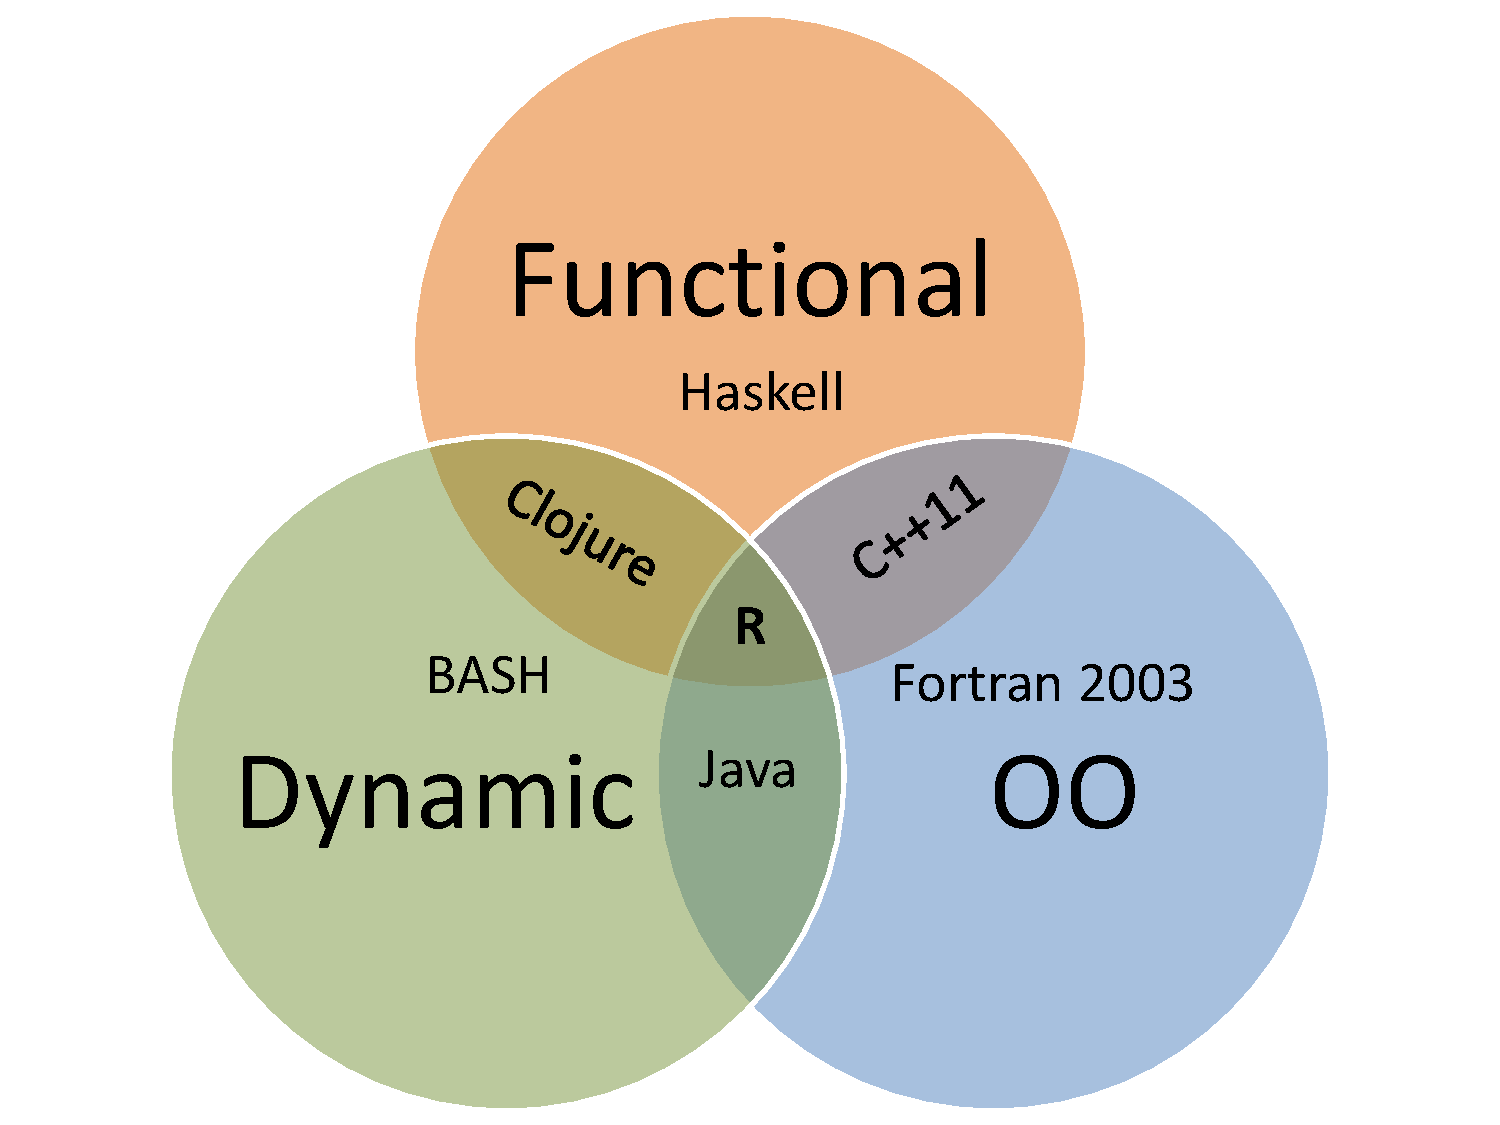
\includegraphics[scale=.35]{../common/pics/languages}
  \end{center}
  \end{block}
\end{frame}

\begin{frame}
  \begin{block}{Data Types}\pause
  \begin{itemize}[<+-|alert@+>]
    \item Storage:  logical, int, double, double complex, character
    \item Structures:  vector, matrix, array, list, dataframe
    \item Caveats:  (Logical) \code{TRUE}, \code{FALSE}, \code{NA}
  \end{itemize}
  For the remainder of the tutorial, we will restrict ourselves to real number 
matrix computations.
\end{block}
\end{frame}




\subsection{Syntax for Data Science}


\begin{frame}[fragile]
\begin{block}{High Level Syntax}\pause
\begin{lstlisting}
x <- matrix(rnorm(30), nrow=10)
x <- x[-1, 2:5]
x <- log(abs(x) + 1)
xtx <- t(x) %*% x
ans <- svd(solve(xtx))
\end{lstlisting}
\end{block}
\end{frame}


\begin{frame}
  \begin{block}{More than just a Matlab clone\dots}\pause
  \begin{itemize}[<+-|alert@+>]
    \item Data science (machine learning, statistics, data mining, \dots) is 
mostly matrix algebra.  \\[.2cm]
     So what about Matlab/Python/Julia/\dots ?
    \item Depends on your ``religion'' 
    \item As a \emph{data analysis} package, R is king.
  \end{itemize}
\end{block}
\end{frame}



\begin{frame}[fragile]
\begin{block}{High Level Syntax \emph{for Data}}\pause
\begin{lstlisting}
pca <- prcomp(x, retx=TRUE, scale=TRUE)
prop_var <- cumsum(pca$sdev)/sum(pca$sdev)
i <- min(which(prop_var > 0.9)) - 1

y <- pca$x[, 1:i]
\end{lstlisting}
\end{block}
\end{frame}

















\section{Parallel Hardware and R}

\hidenum
\begin{frame}[noframenumbering]
\frametitle{Contents}
 \tableofcontents[currentsection,hideothersubsections,sectionstyle=show/hide]
\end{frame}
\shownum

\subsection{Parallel Hardware}

% \begin{frame}
% \begin{block}{A}
%   
% \end{block}
% \end{frame}


\begin{frame}
\begin{block}{Three Basic Flavors of Hardware}
    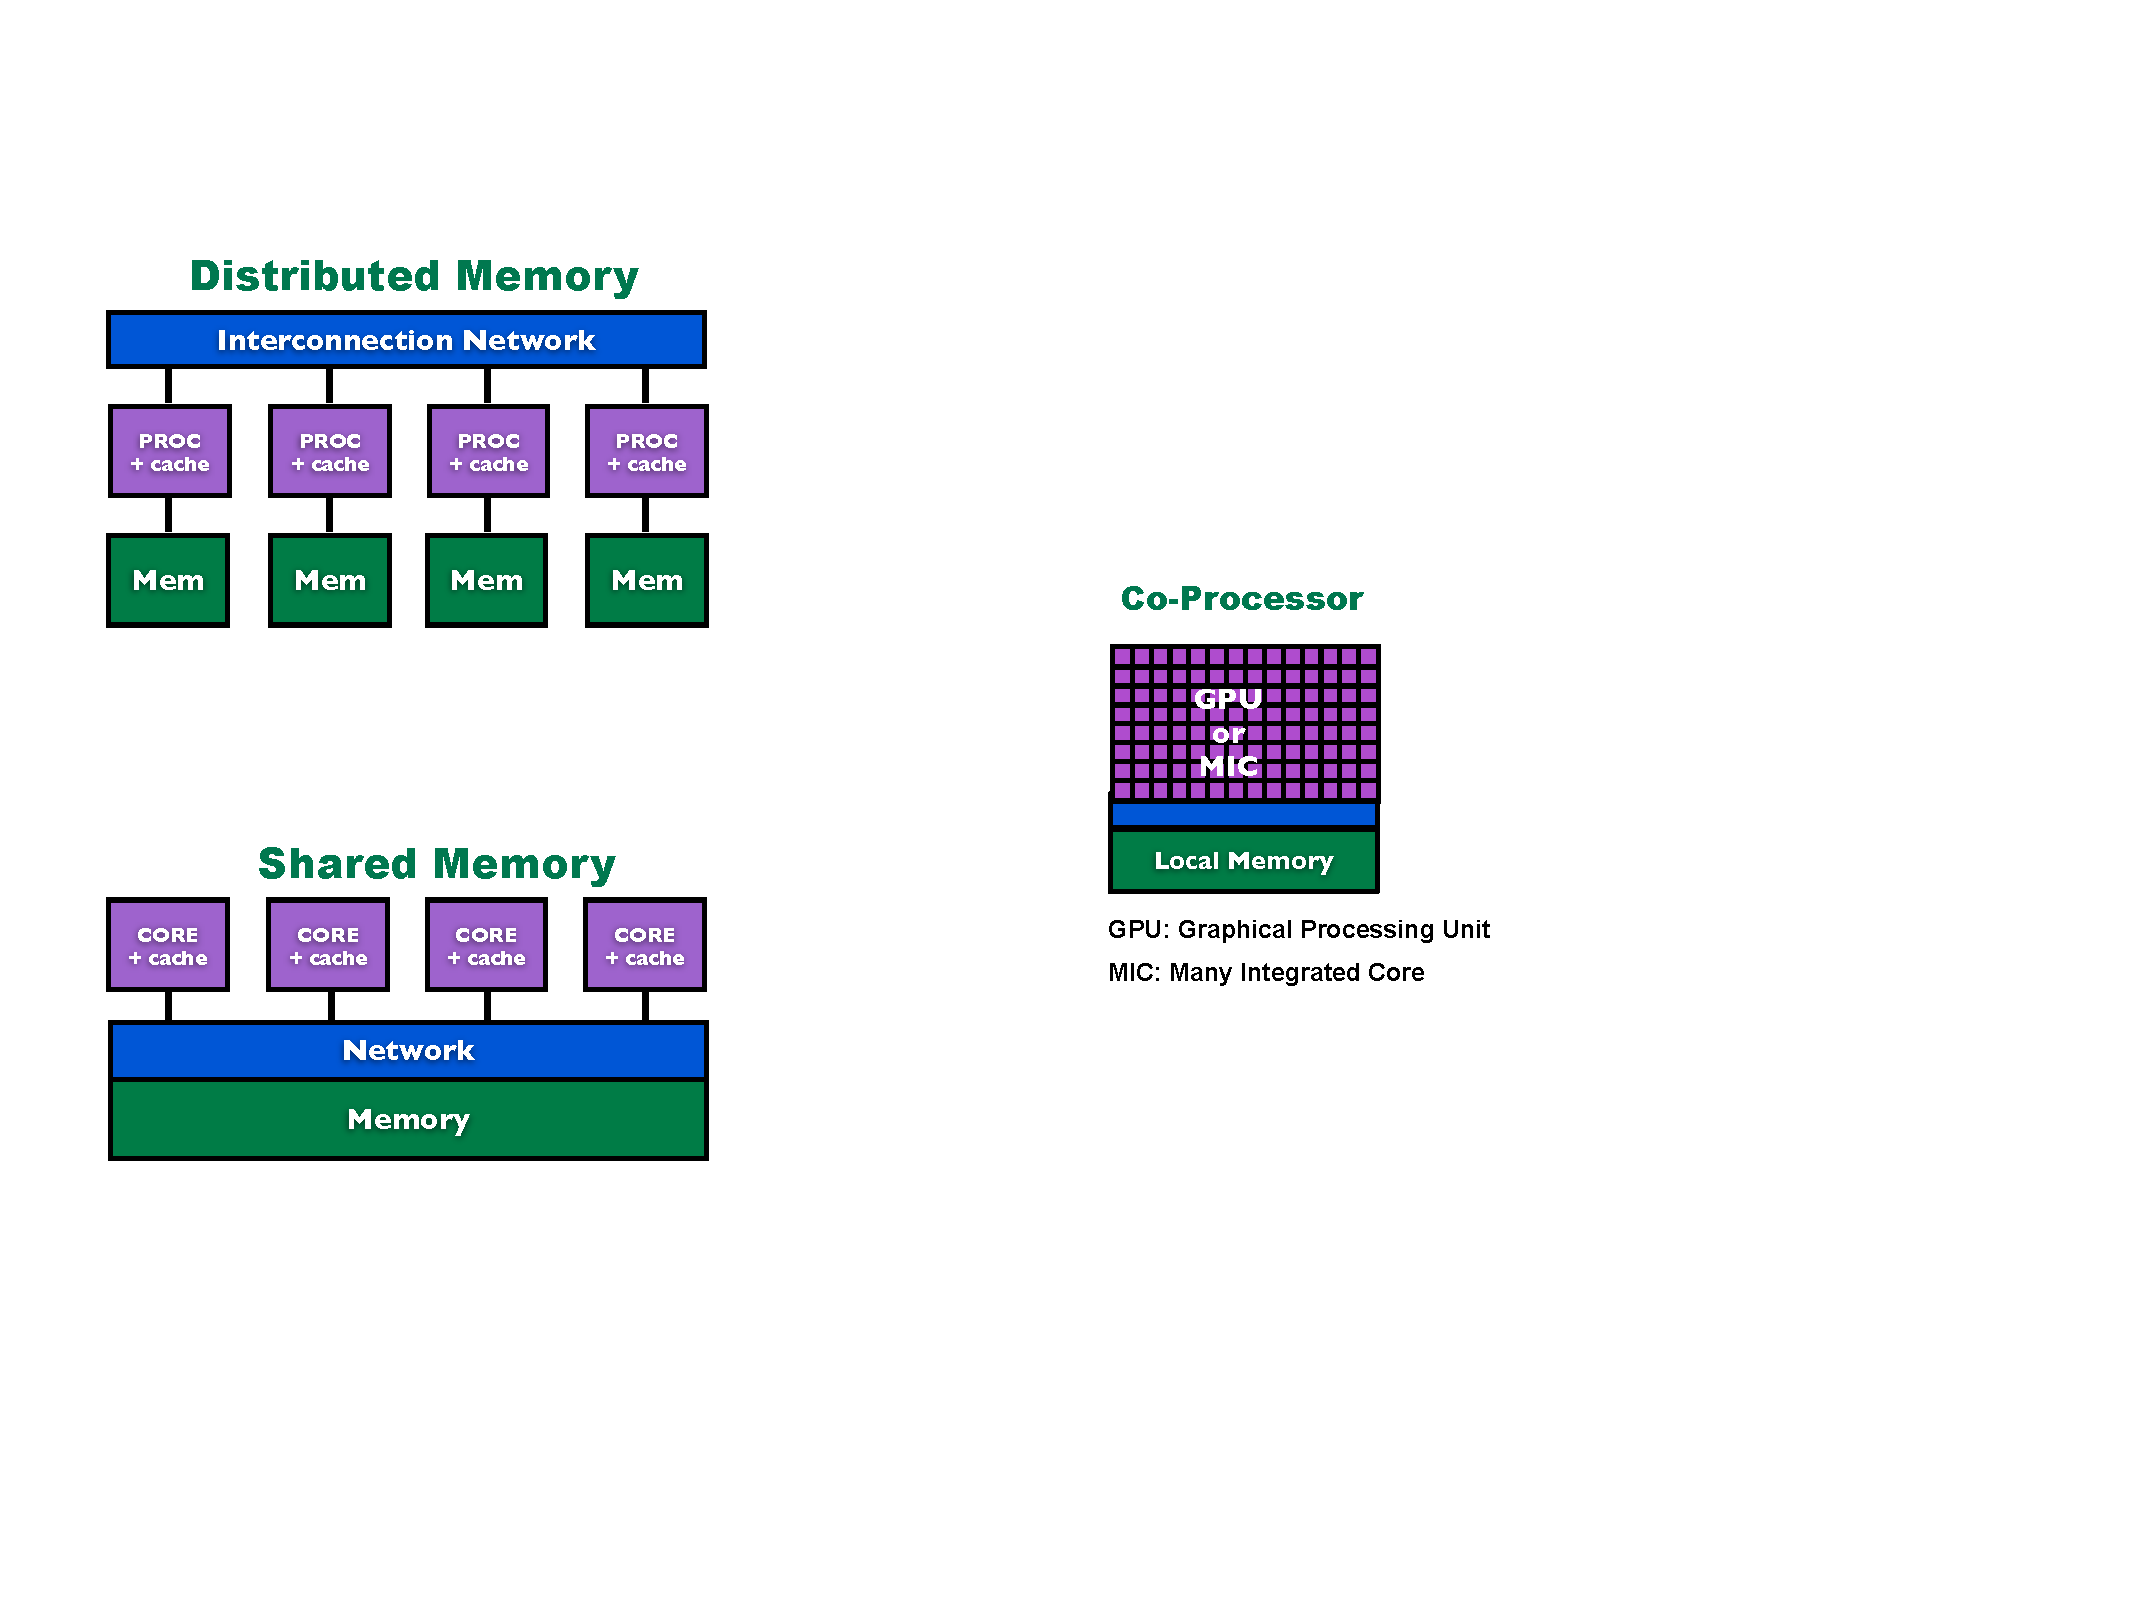
\includegraphics[width=0.95\textwidth]{../common/pics/ParallelHardware1.pdf}
\end{block}
\end{frame}

\begin{frame}
\begin{block}{Your Laptop or Desktop}
    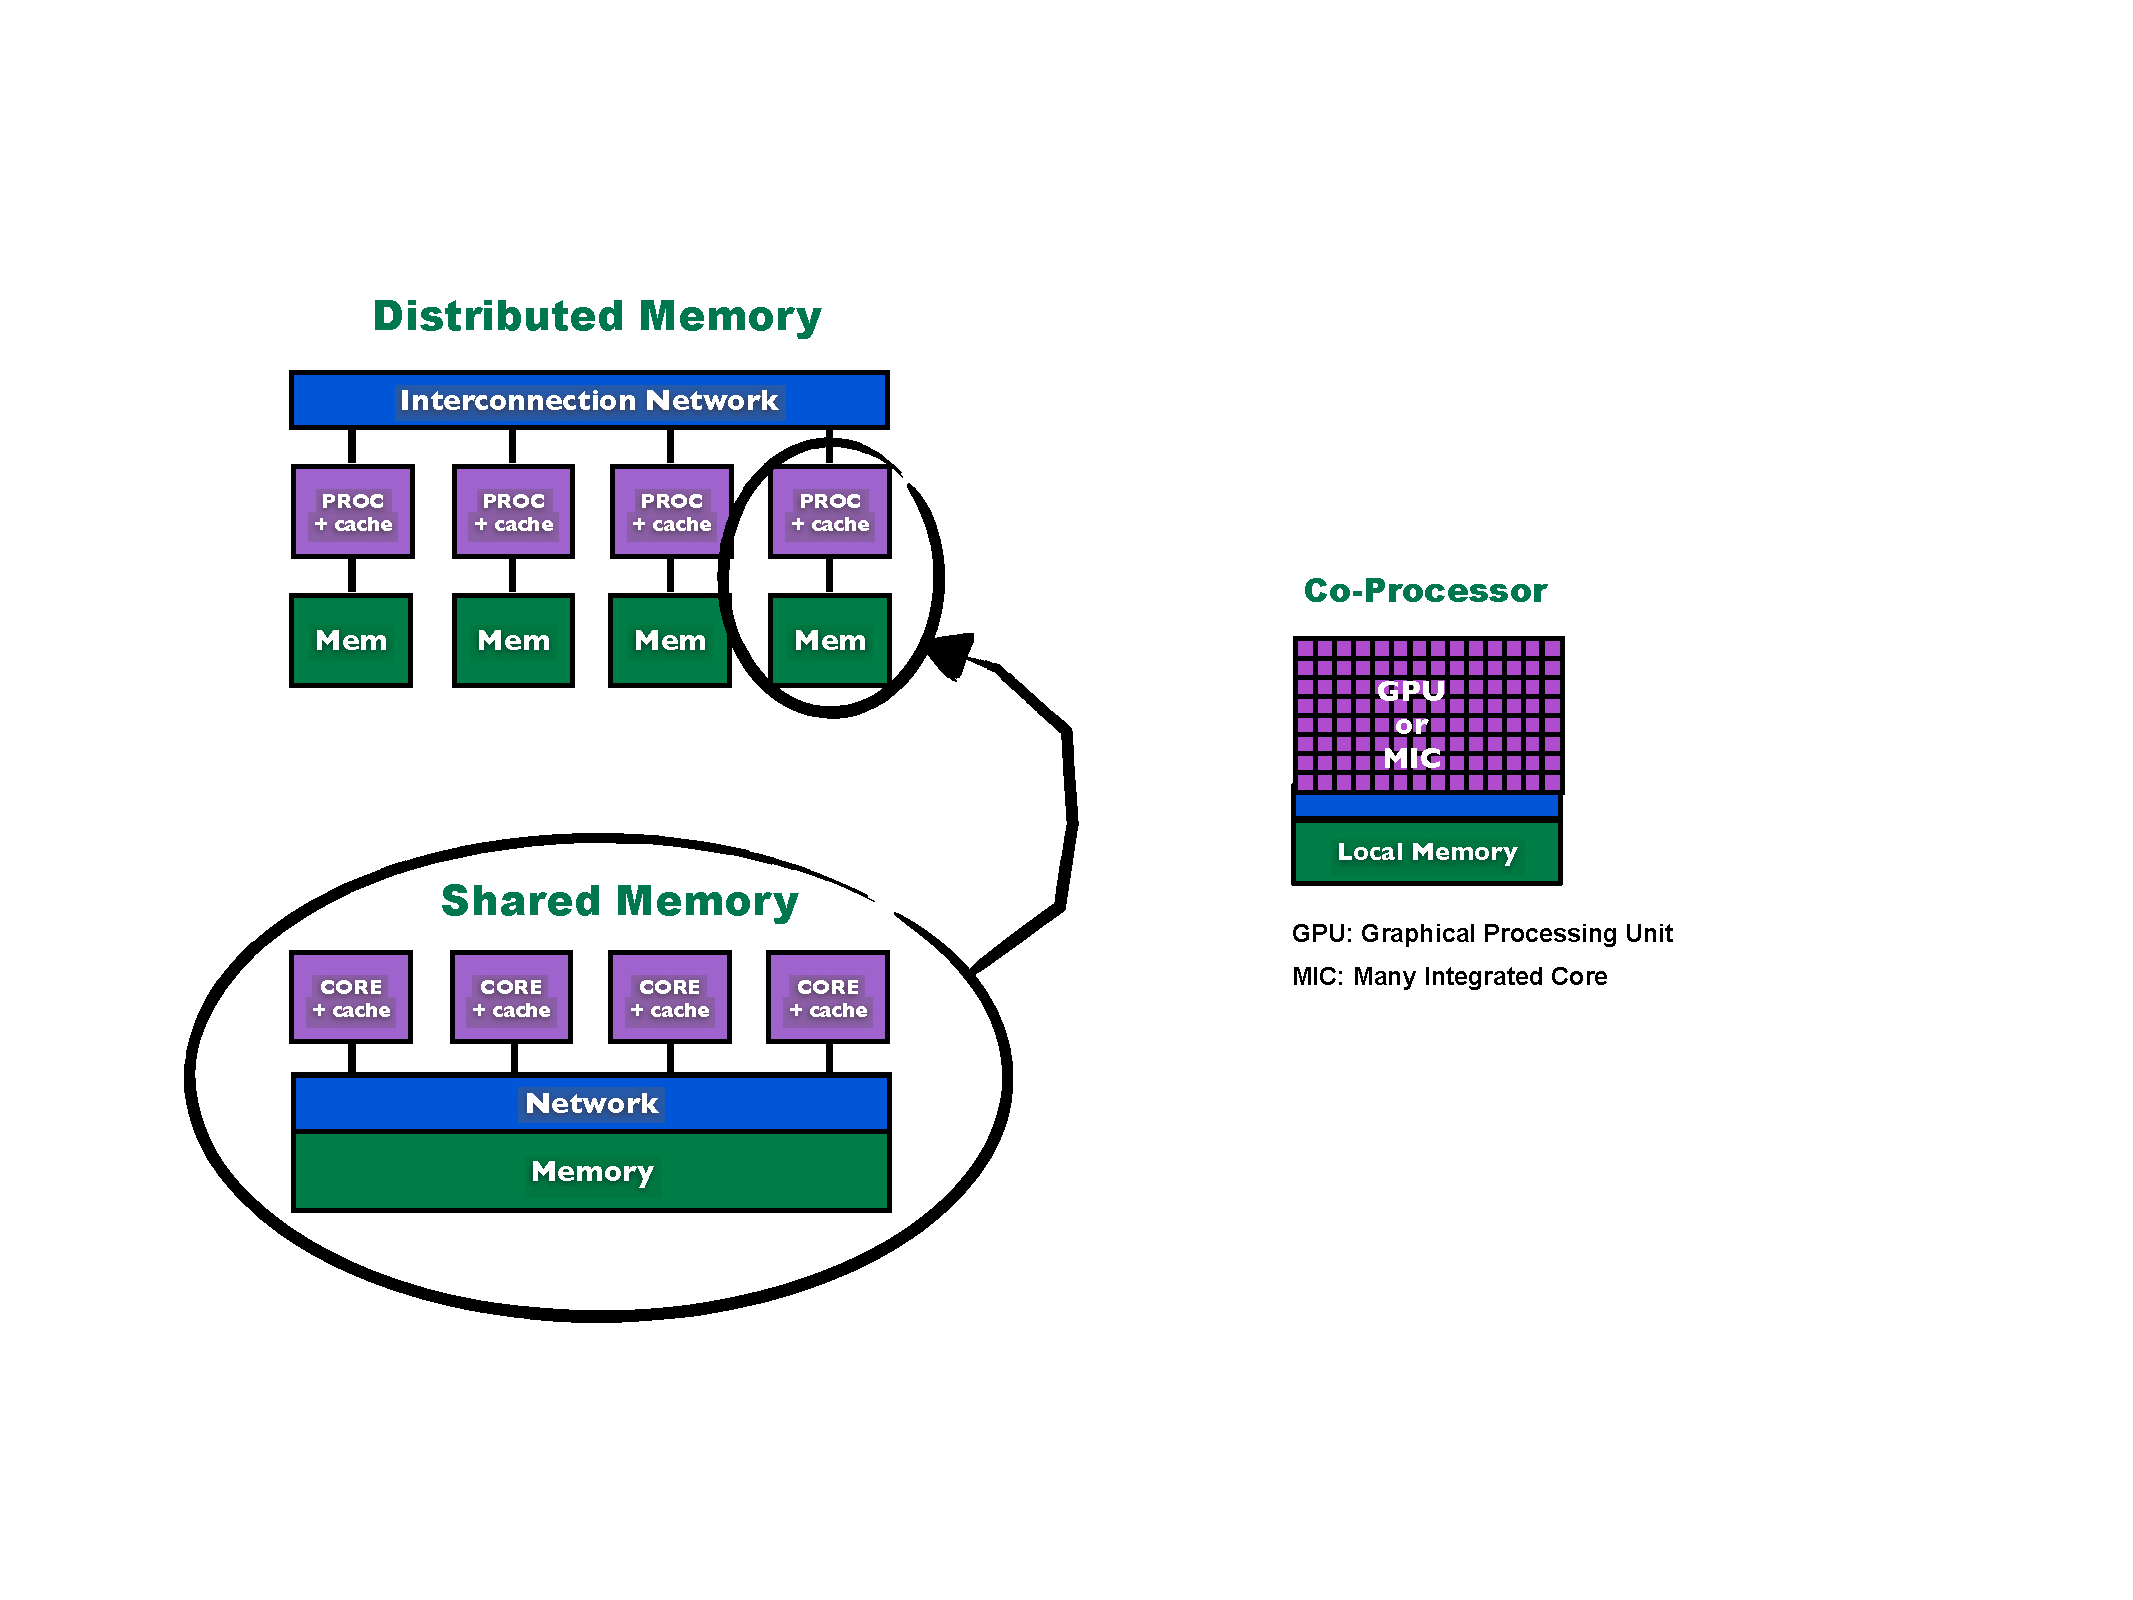
\includegraphics[width=0.95\textwidth]{../common/pics/ParallelHardware2.pdf}
\end{block}
\end{frame}

\begin{frame}
\begin{block}{A Server or Cluster}
    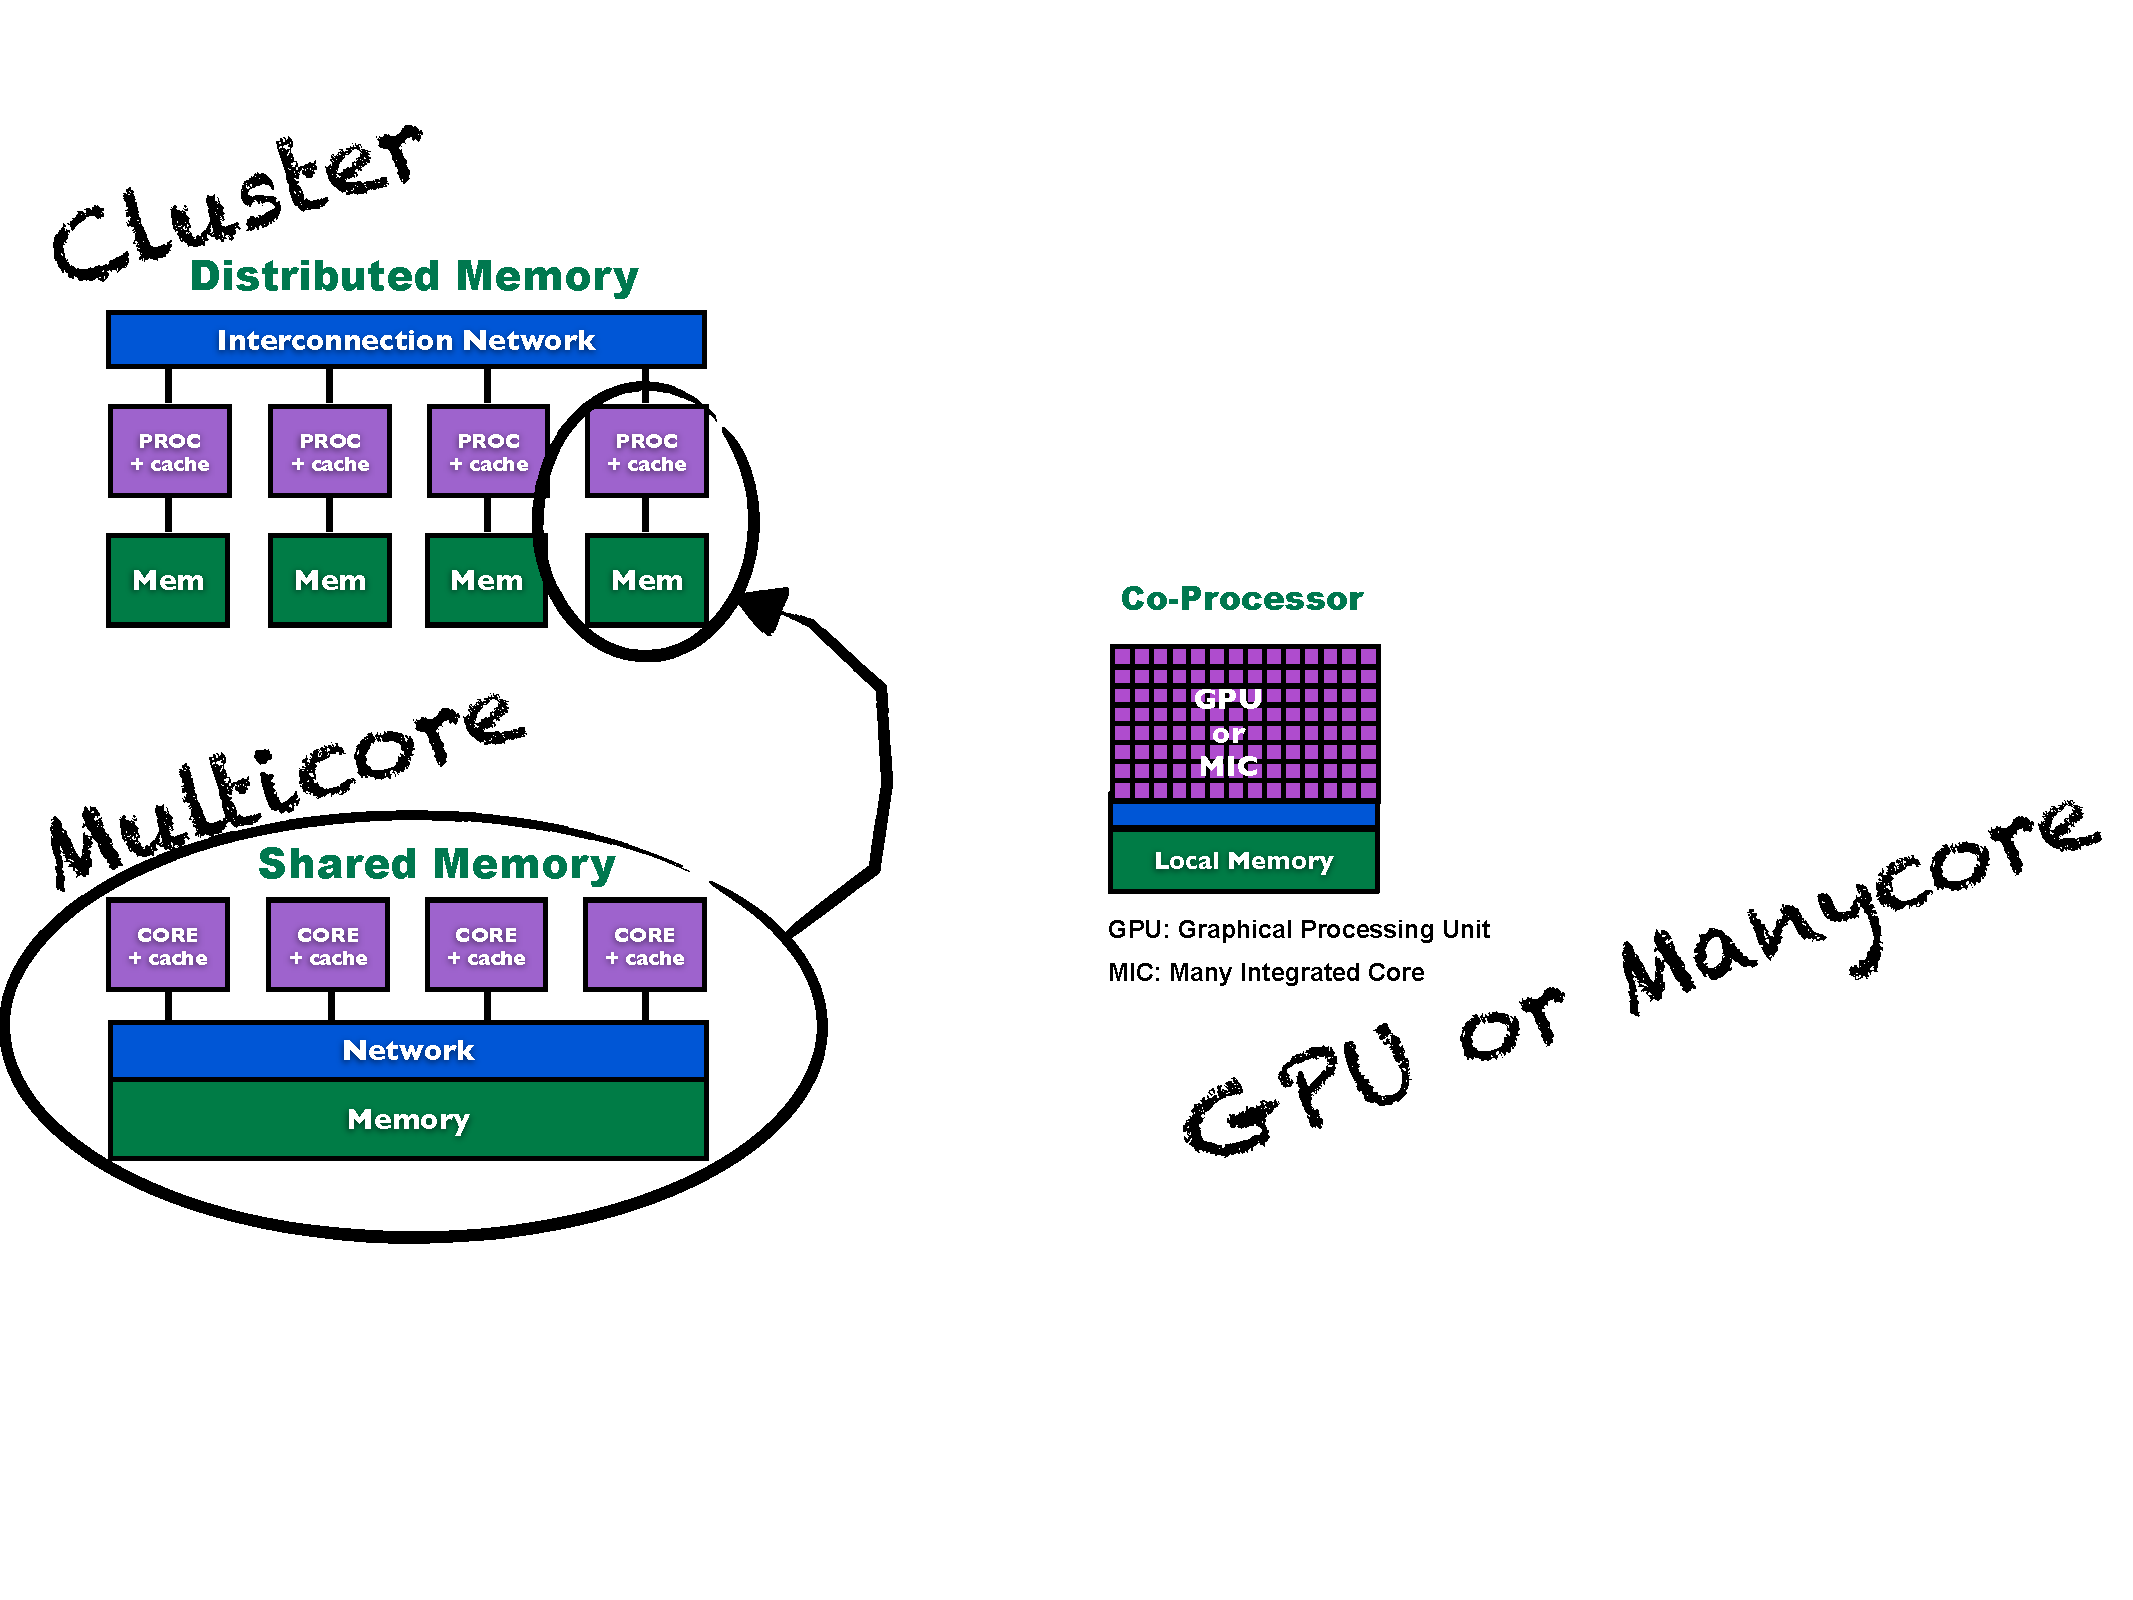
\includegraphics[width=0.95\textwidth]{../common/pics/ParallelHardware3.pdf}
\end{block}
\end{frame}

\begin{frame}
\begin{block}{Server to Supercomputer}
    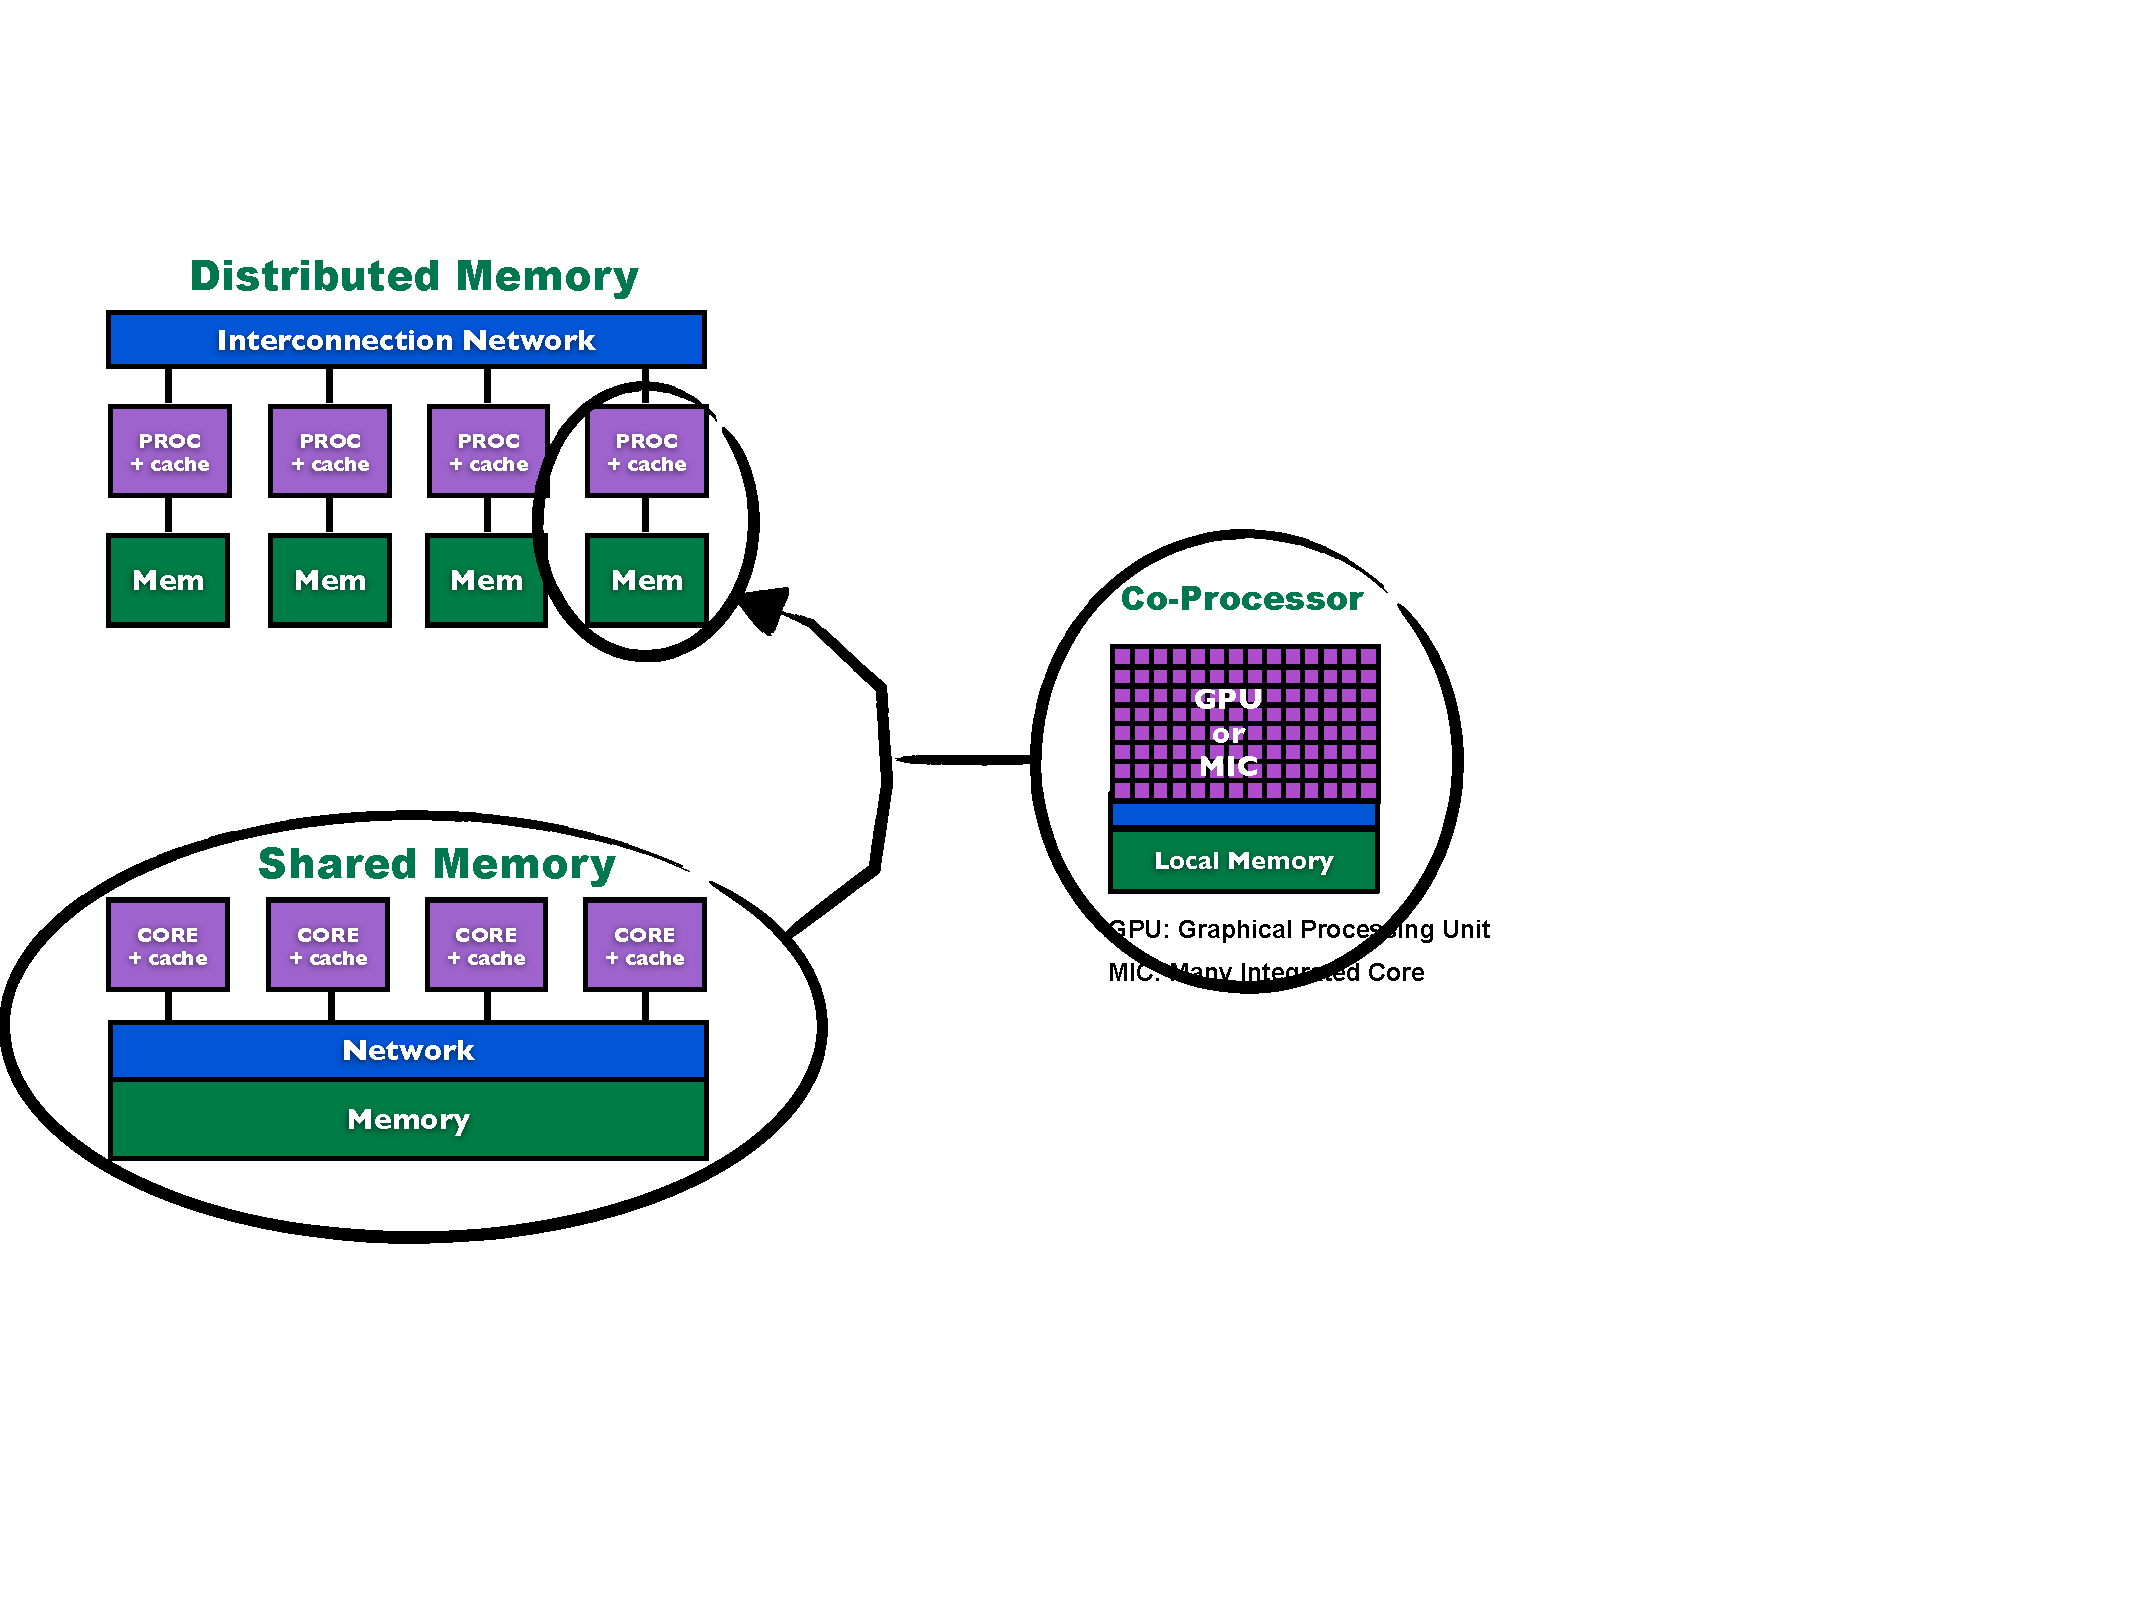
\includegraphics[width=0.95\textwidth]{../common/pics/ParallelHardware4.pdf}
\end{block}
\end{frame}

\begin{frame}
\begin{block}{Knowing the Right Words}
    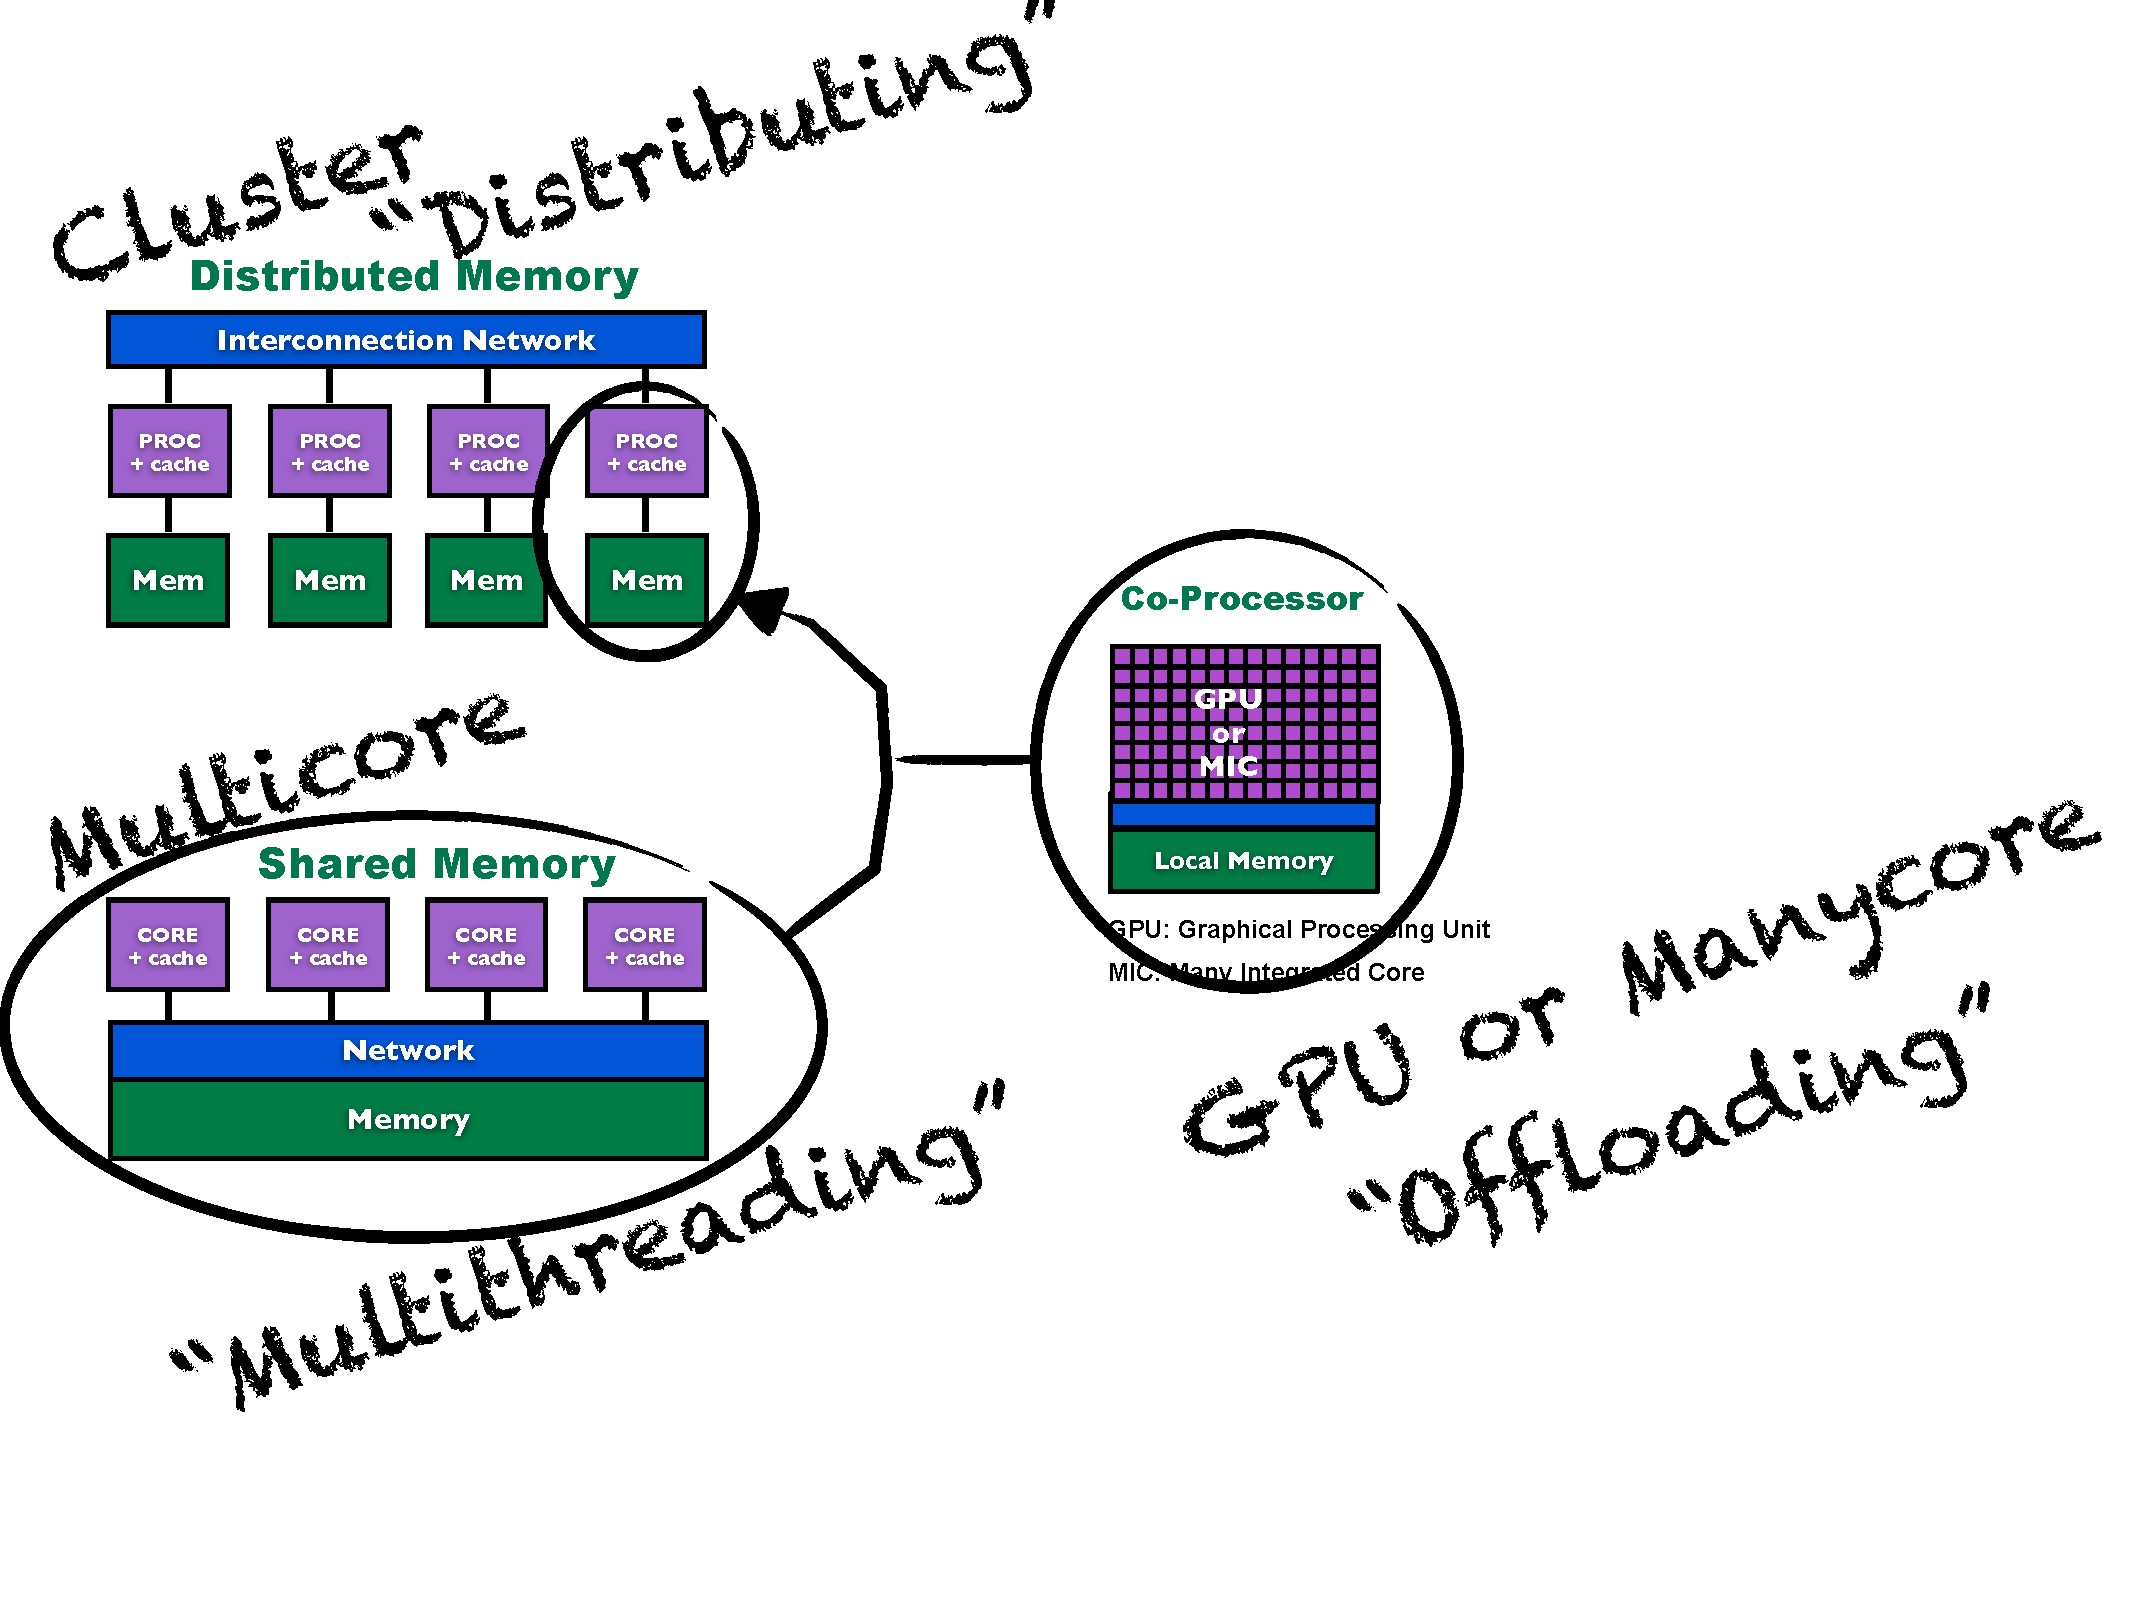
\includegraphics[width=0.95\textwidth]{../common/pics/ParallelHardware5.pdf}
\end{block}
\end{frame}

\begin{frame}
\begin{block}{``Native'' Programming Models and Tools}
    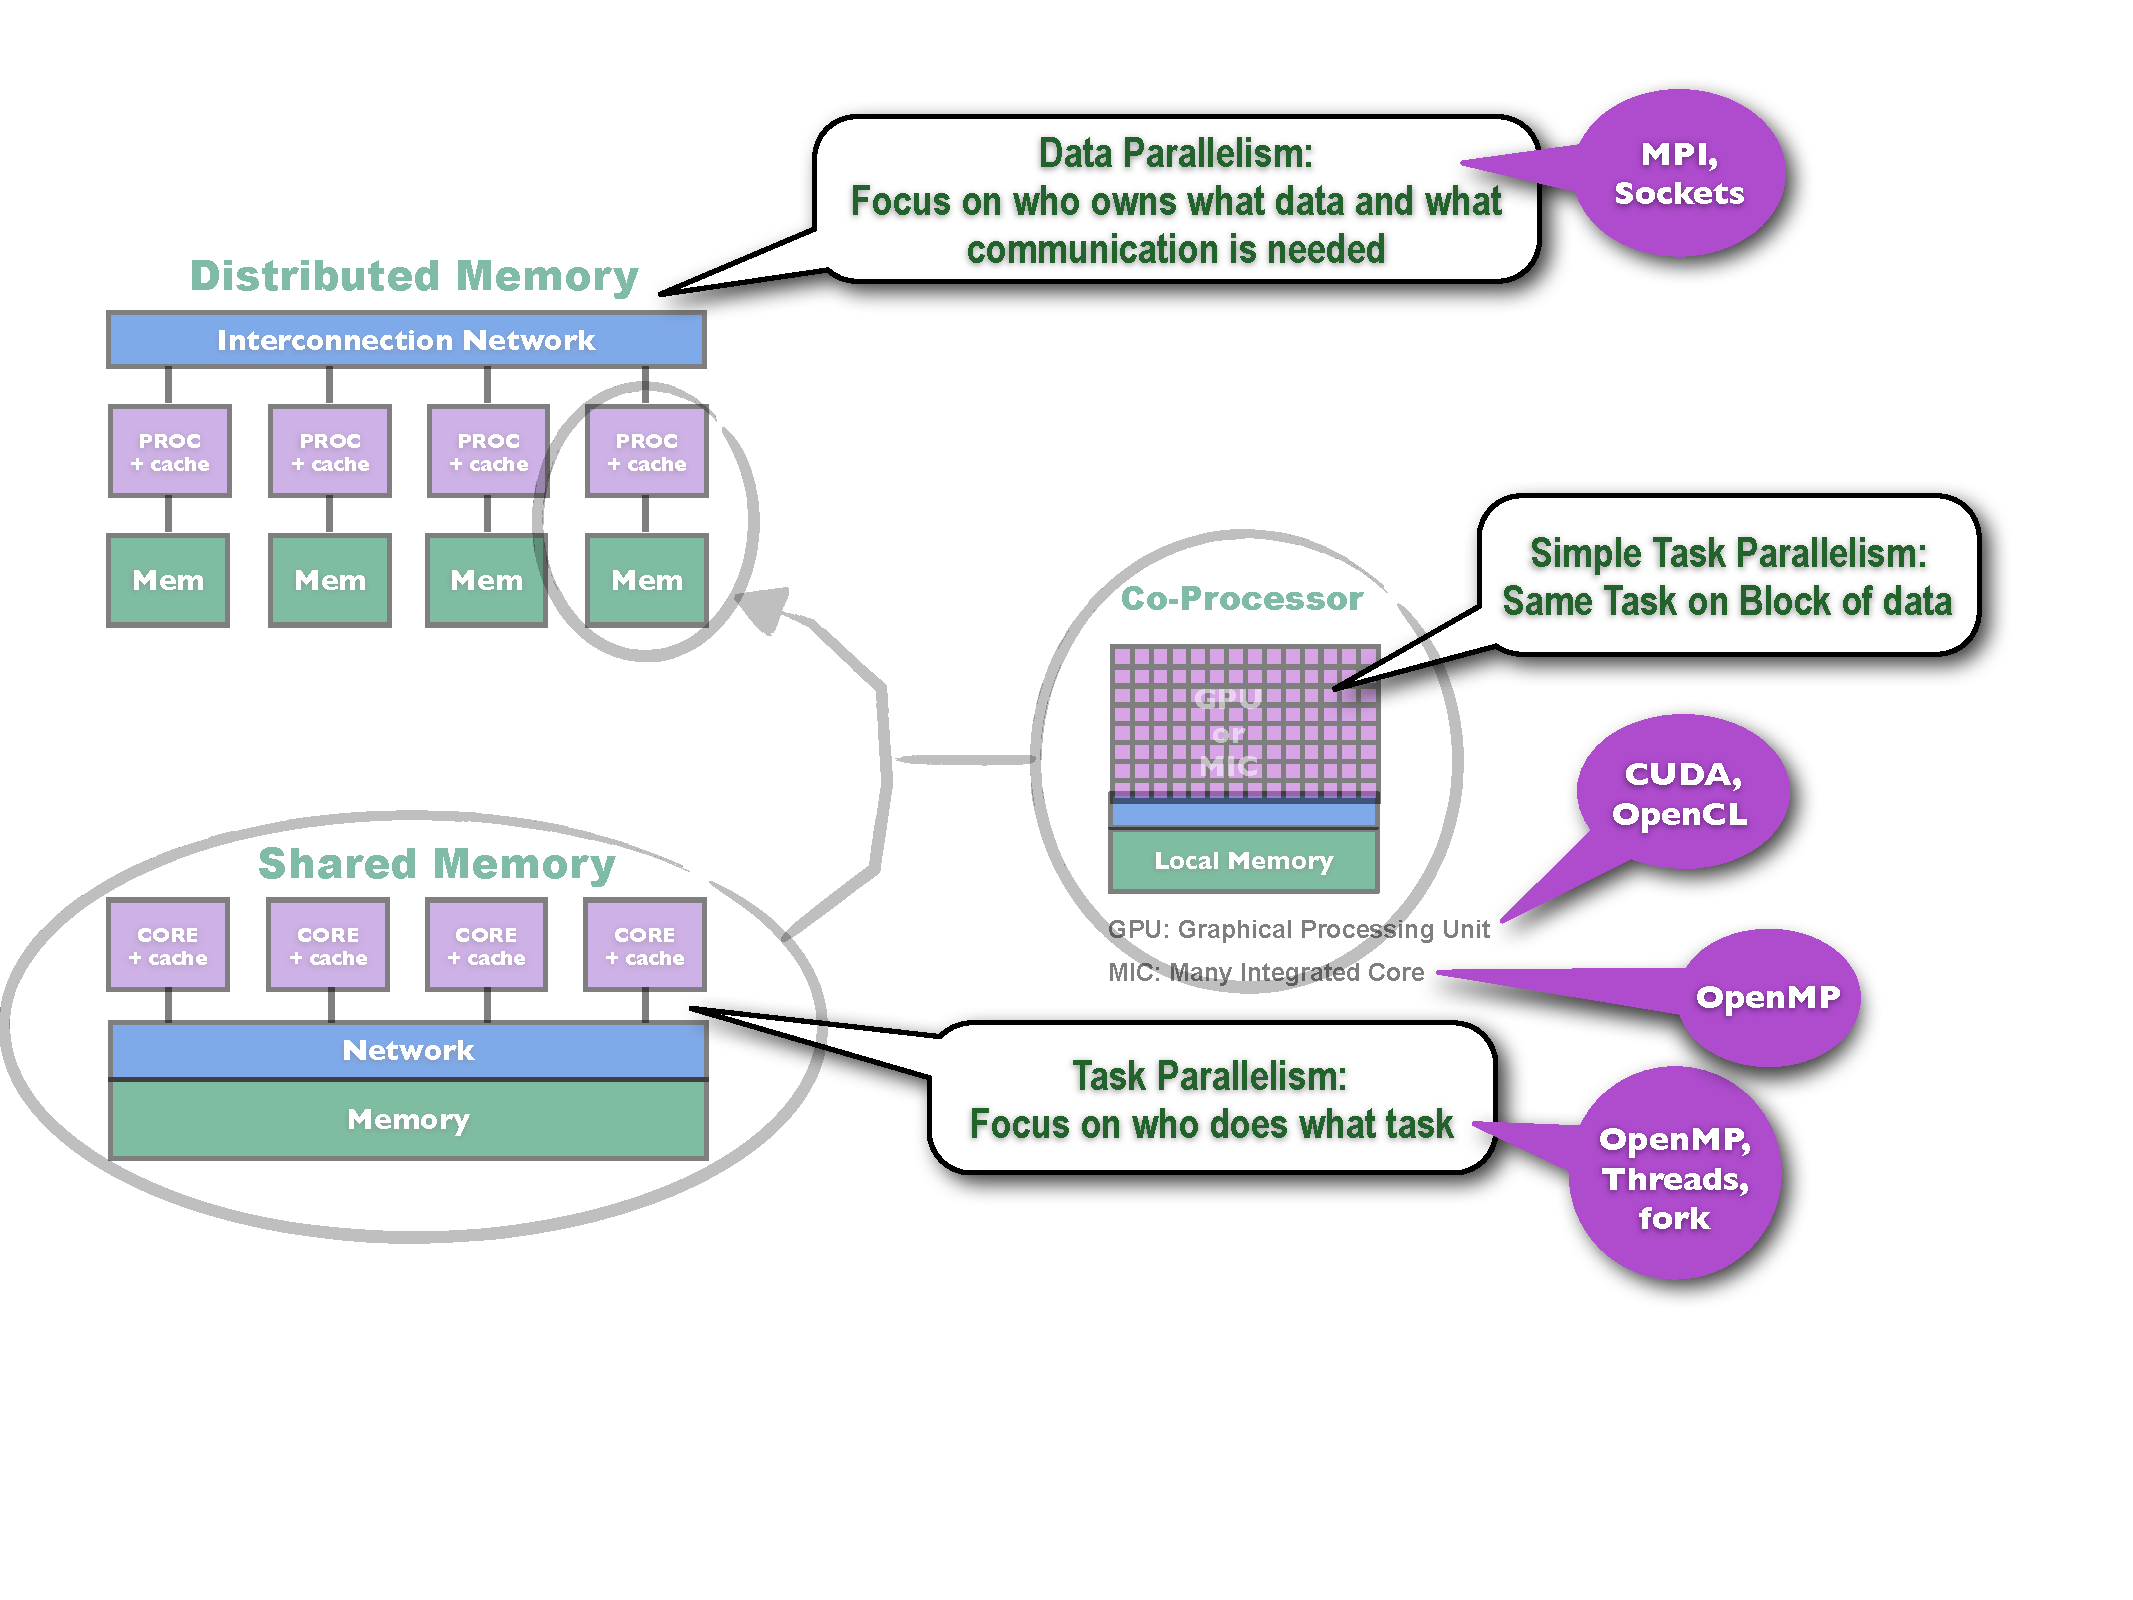
\includegraphics[width=0.95\textwidth]{../common/pics/ParallelHardware6.pdf}
\end{block}
\end{frame}

\subsection{R Interfaces to Parallel Hardware}

\begin{frame}
\begin{block}{R Interfaces to Native Tools}
    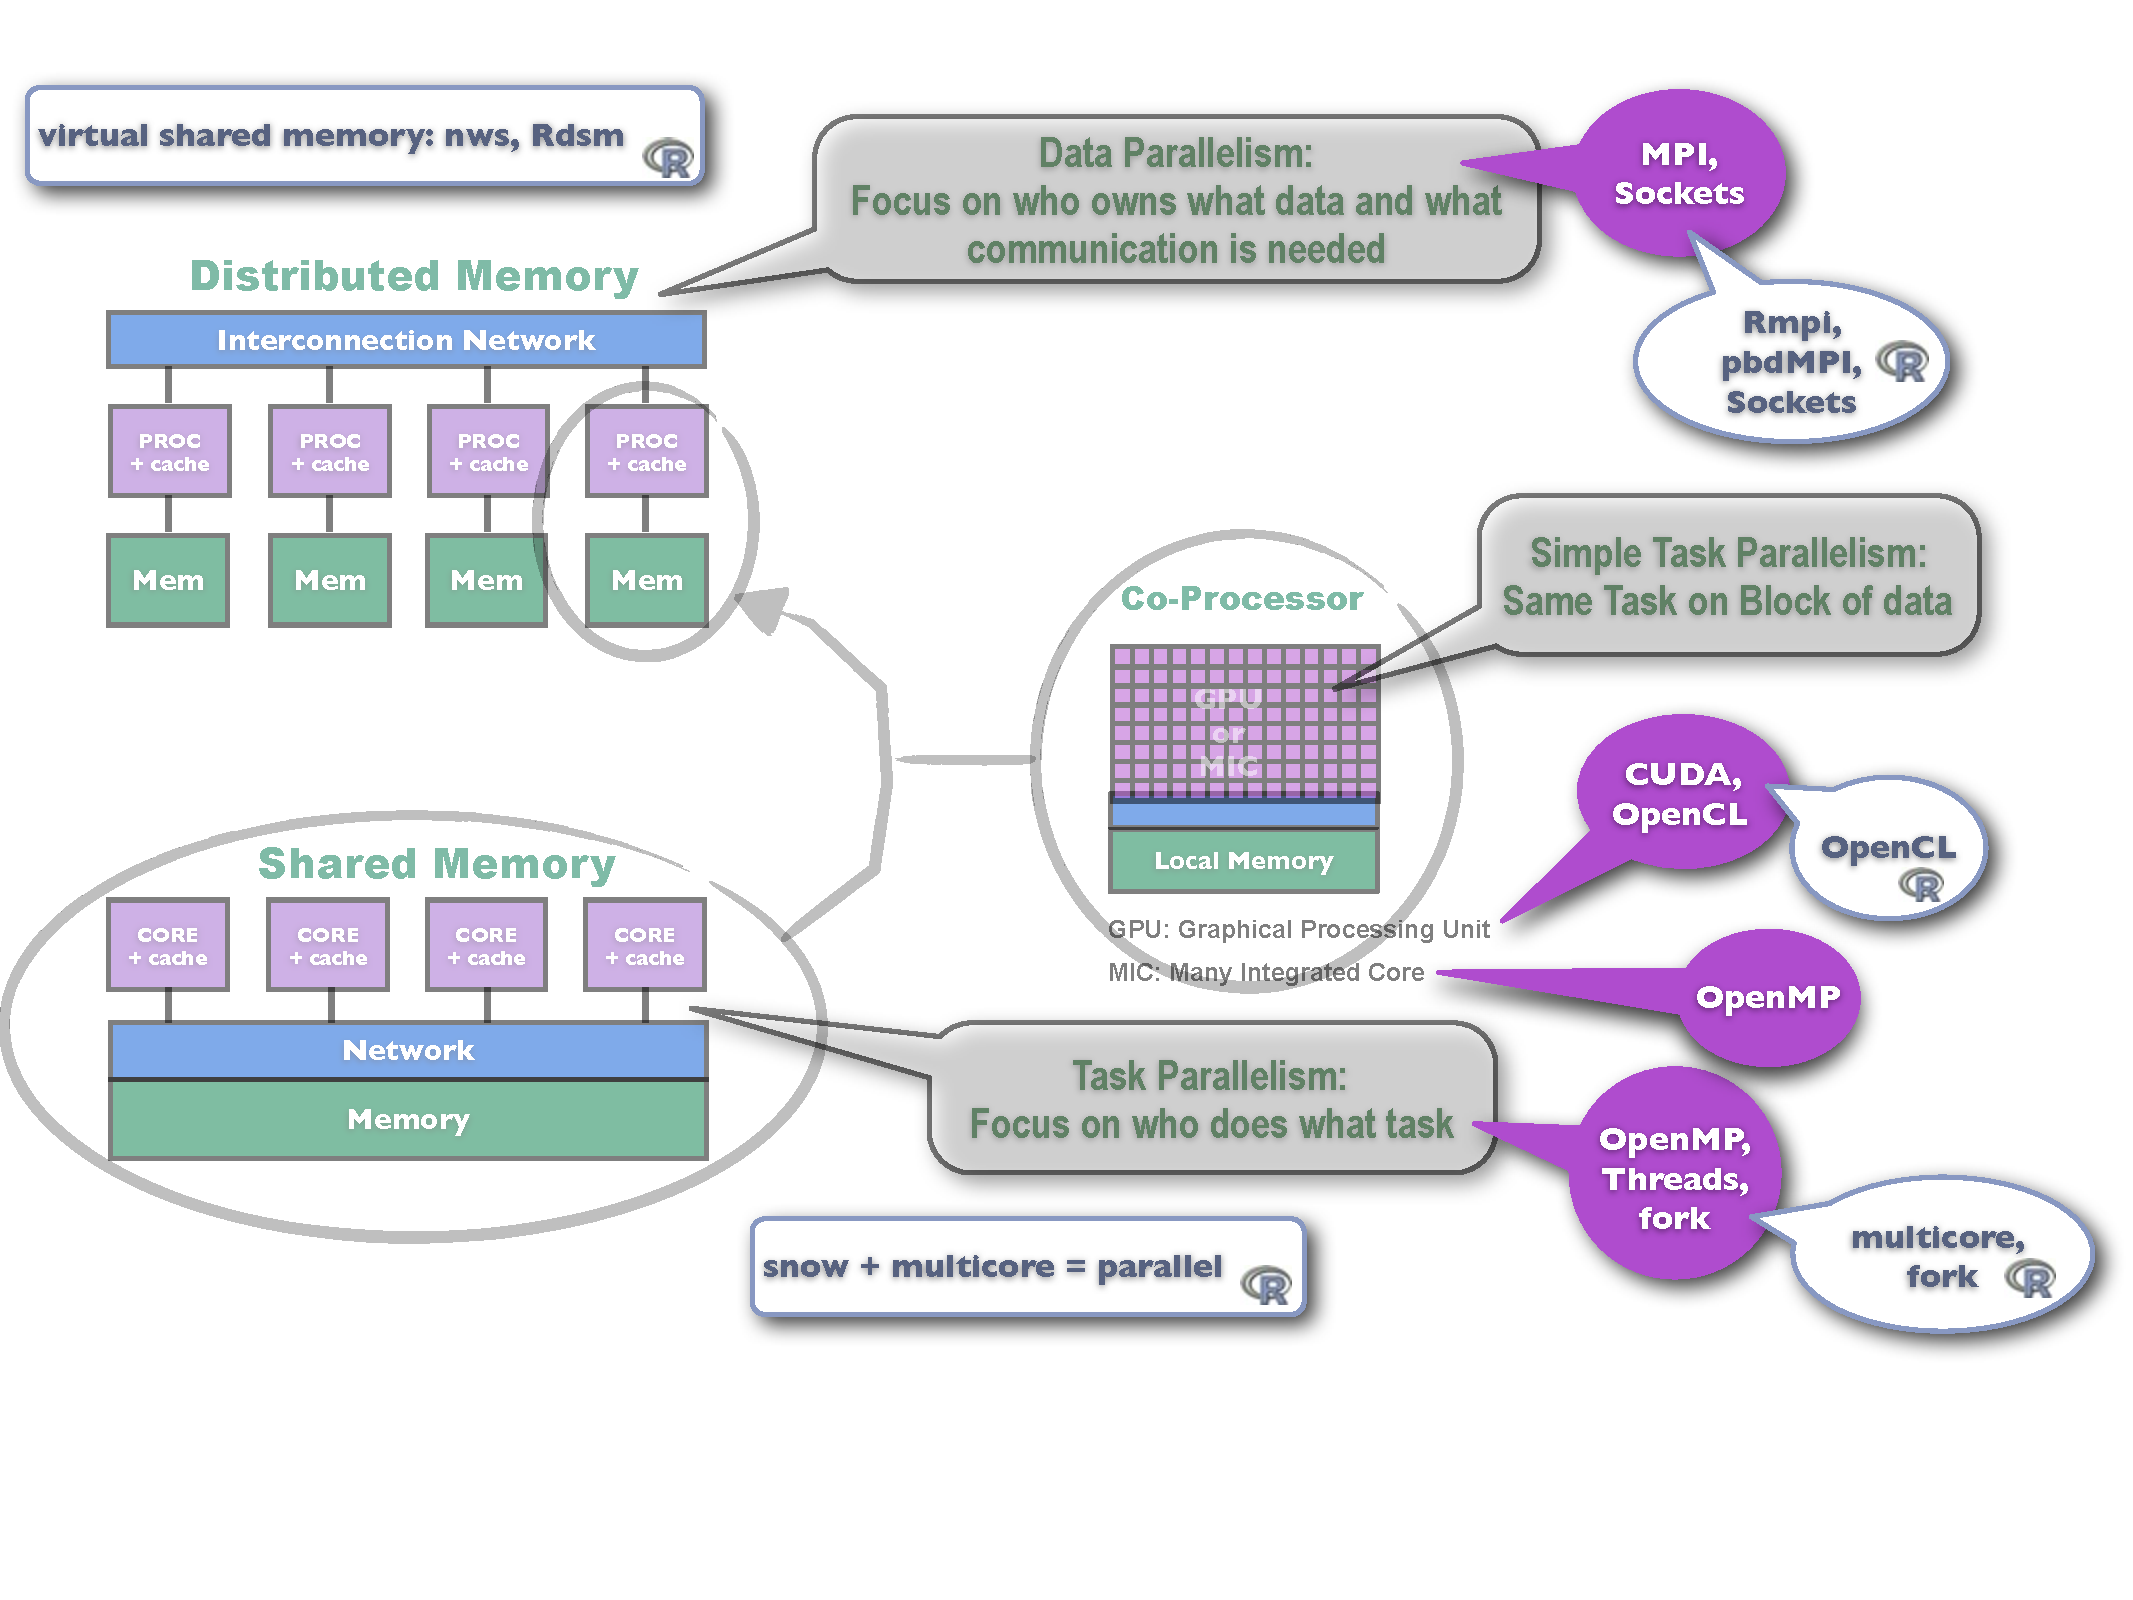
\includegraphics[width=0.95\textwidth]{../common/pics/ParallelHardware7.pdf}
\end{block}
\end{frame}

\begin{frame}
\begin{block}{30+ Years of Parallel Computing Research}
    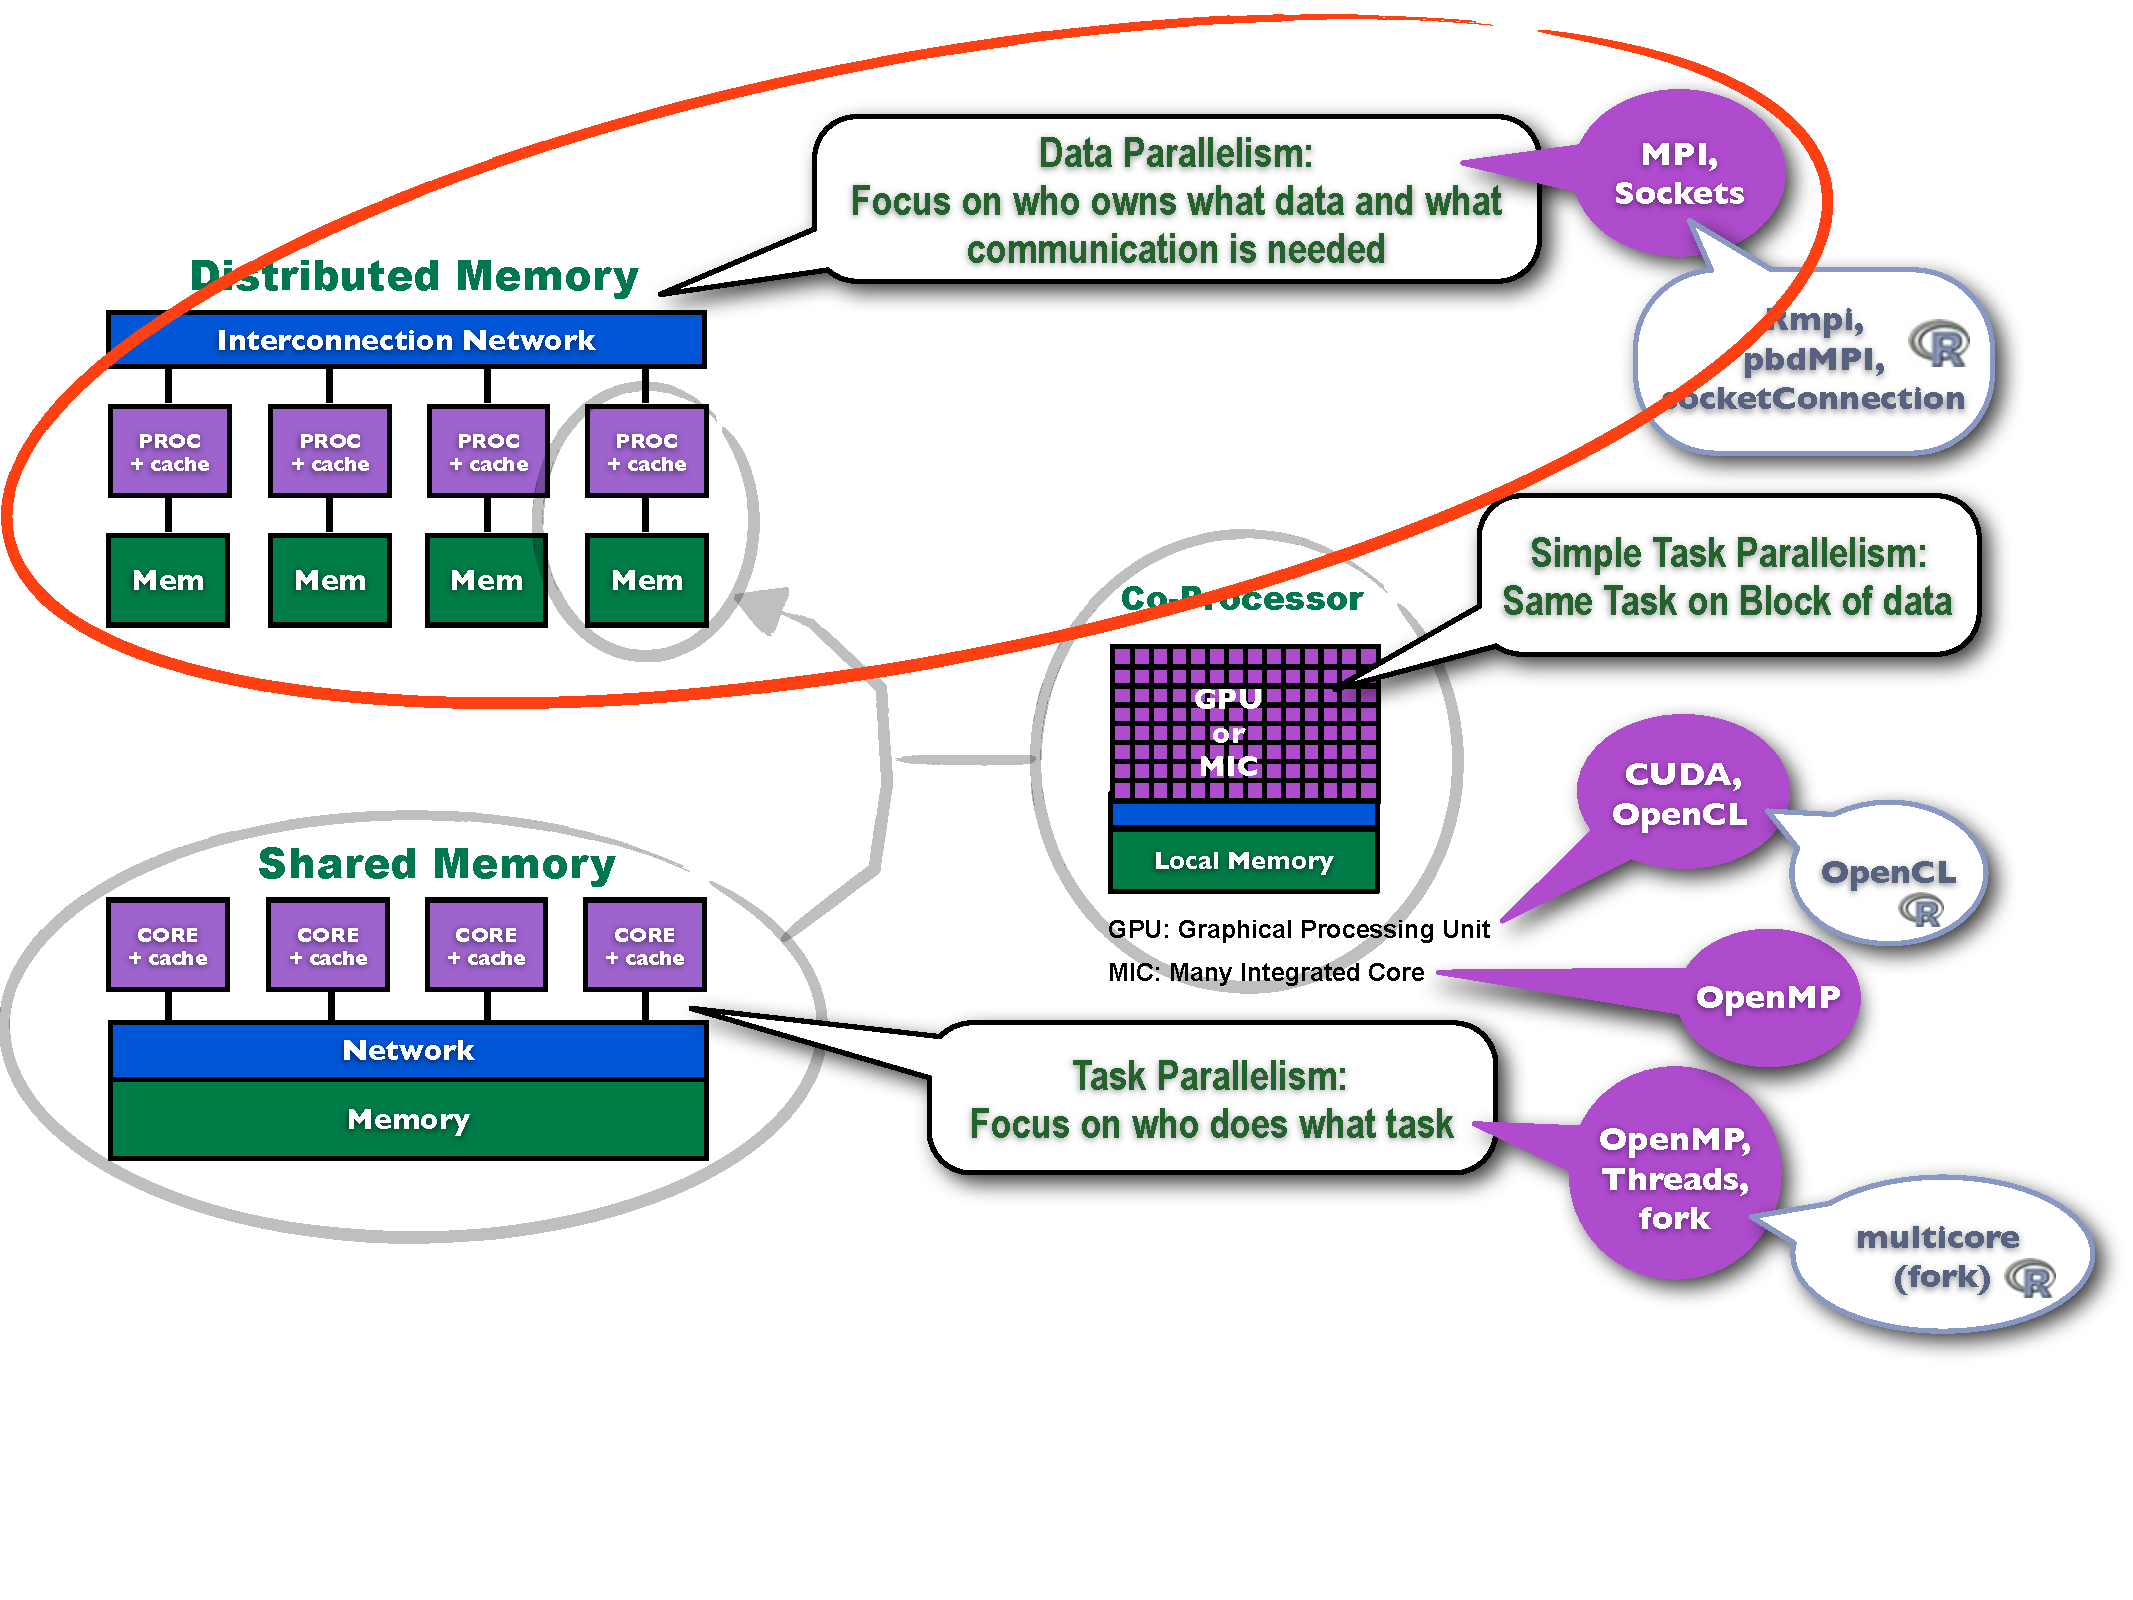
\includegraphics[width=0.95\textwidth]{../common/pics/ParallelHardware8.pdf}
\end{block}
\end{frame}

\begin{frame}
\begin{block}{Last 10 years of Advances}
    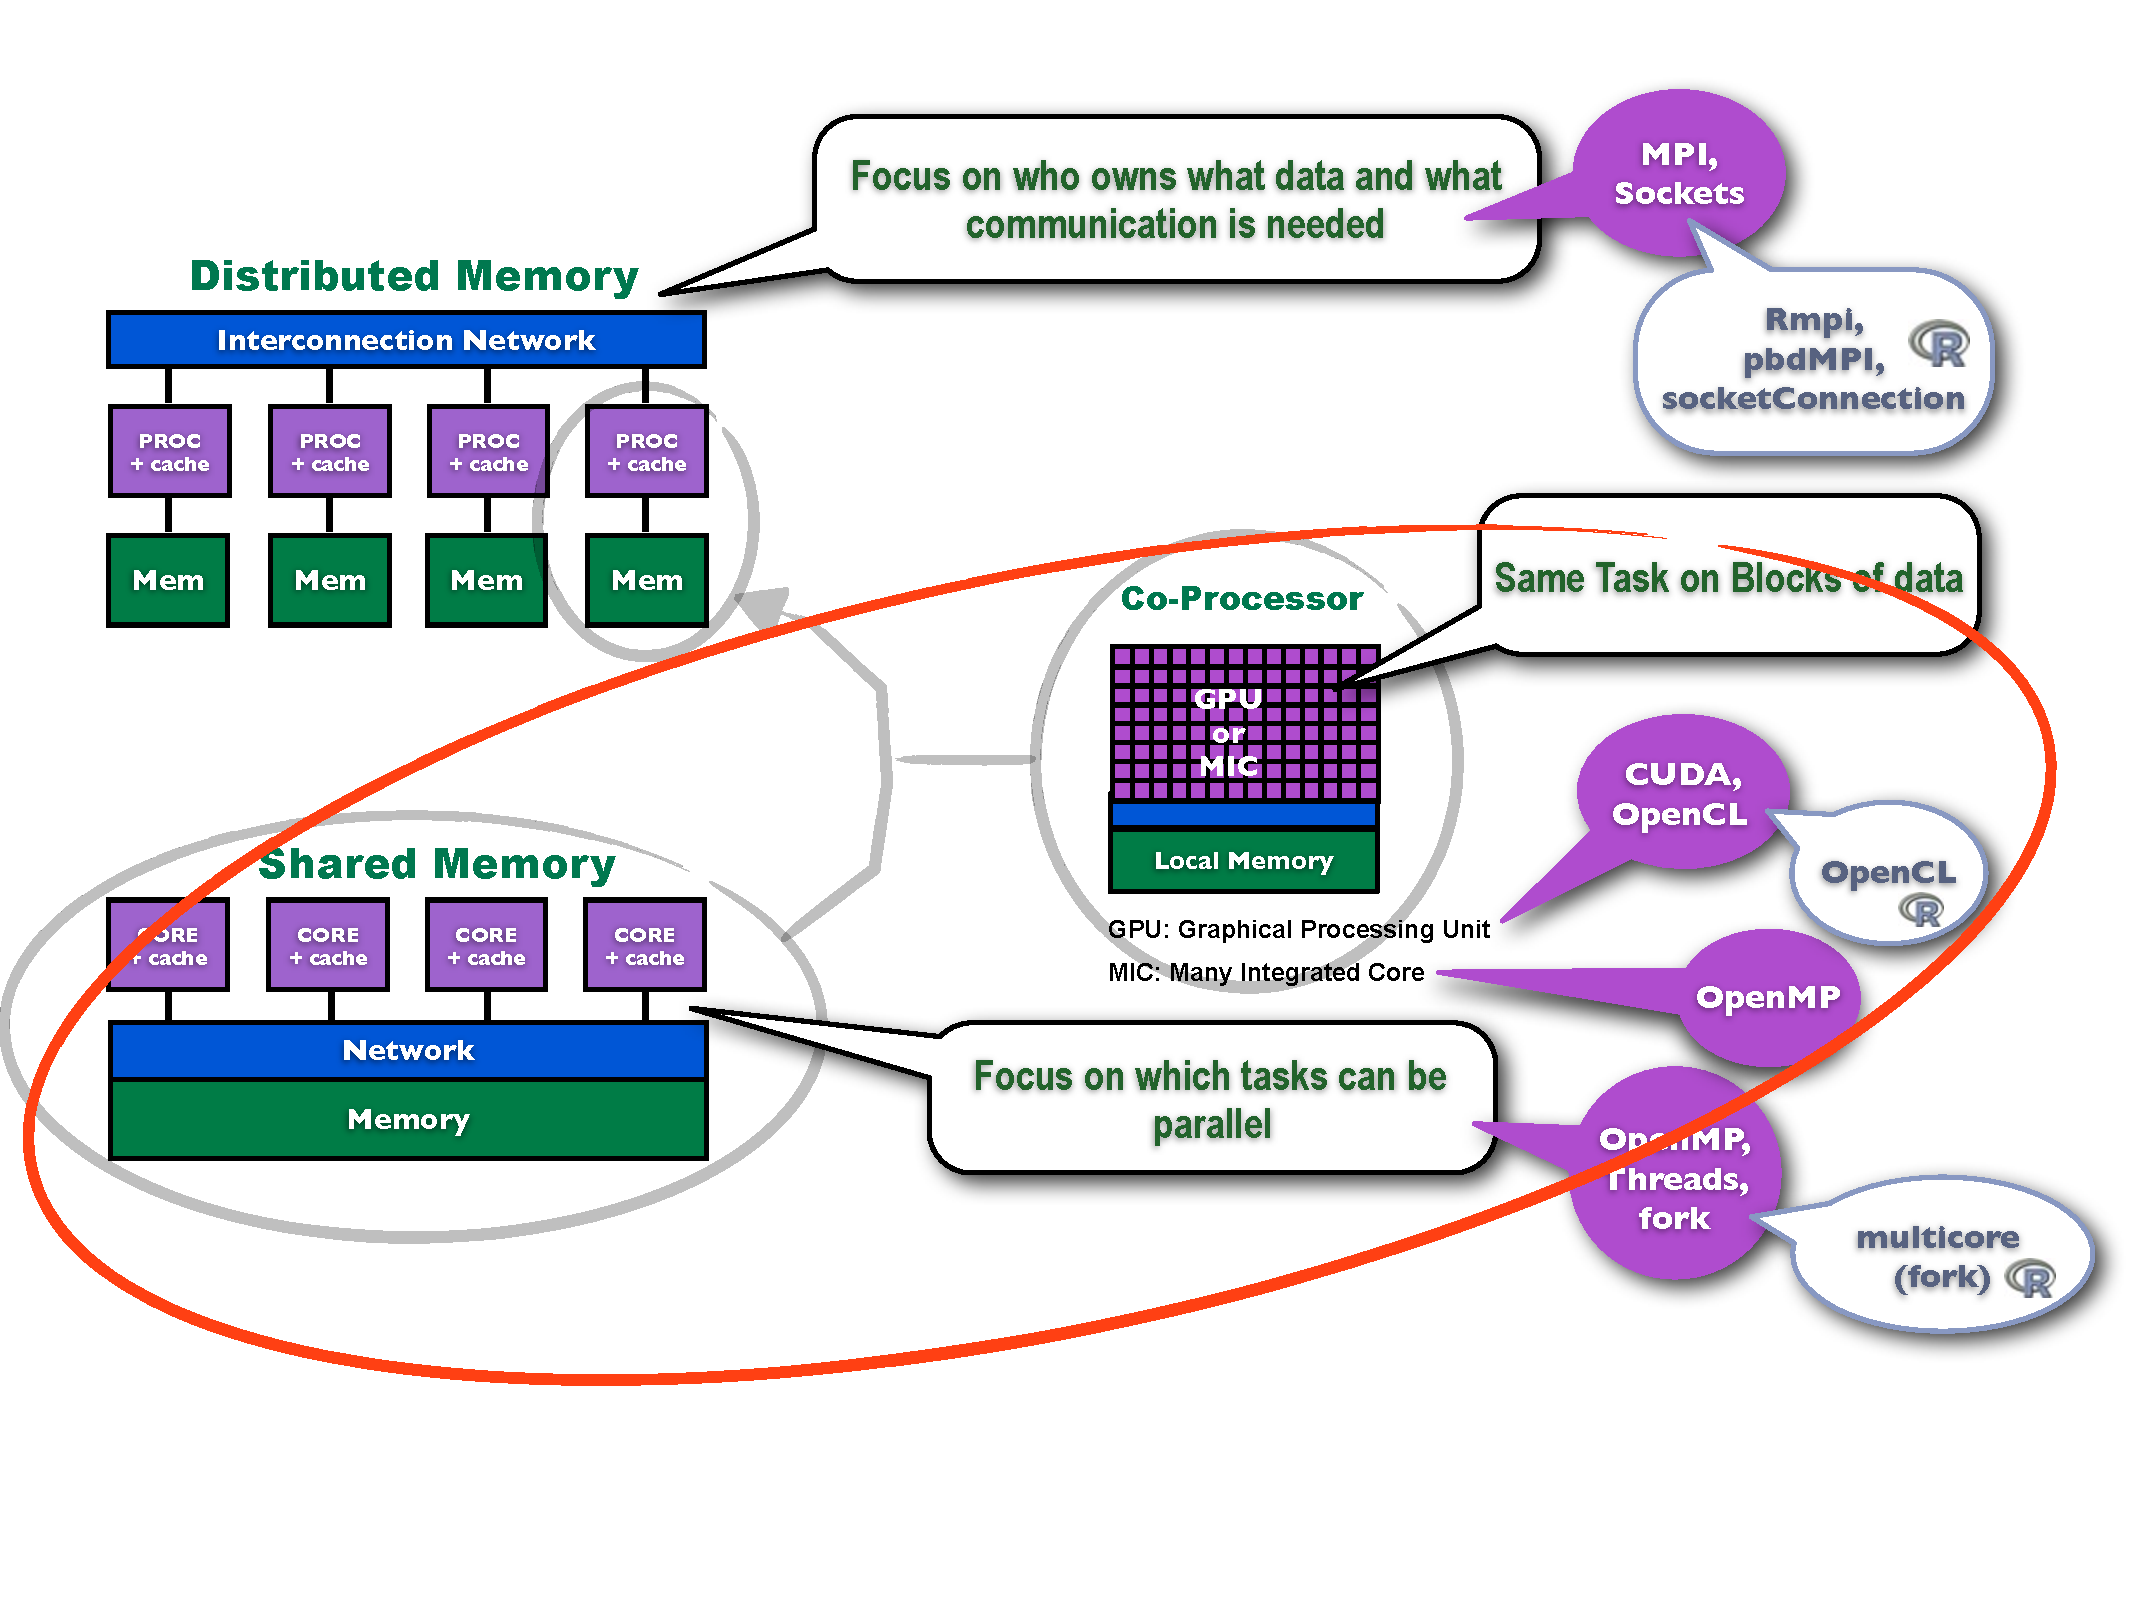
\includegraphics[width=0.95\textwidth]{../common/pics/ParallelHardware9.pdf}
\end{block}
\end{frame}

\begin{frame}
\begin{block}{Putting It All Together Challenge}
    
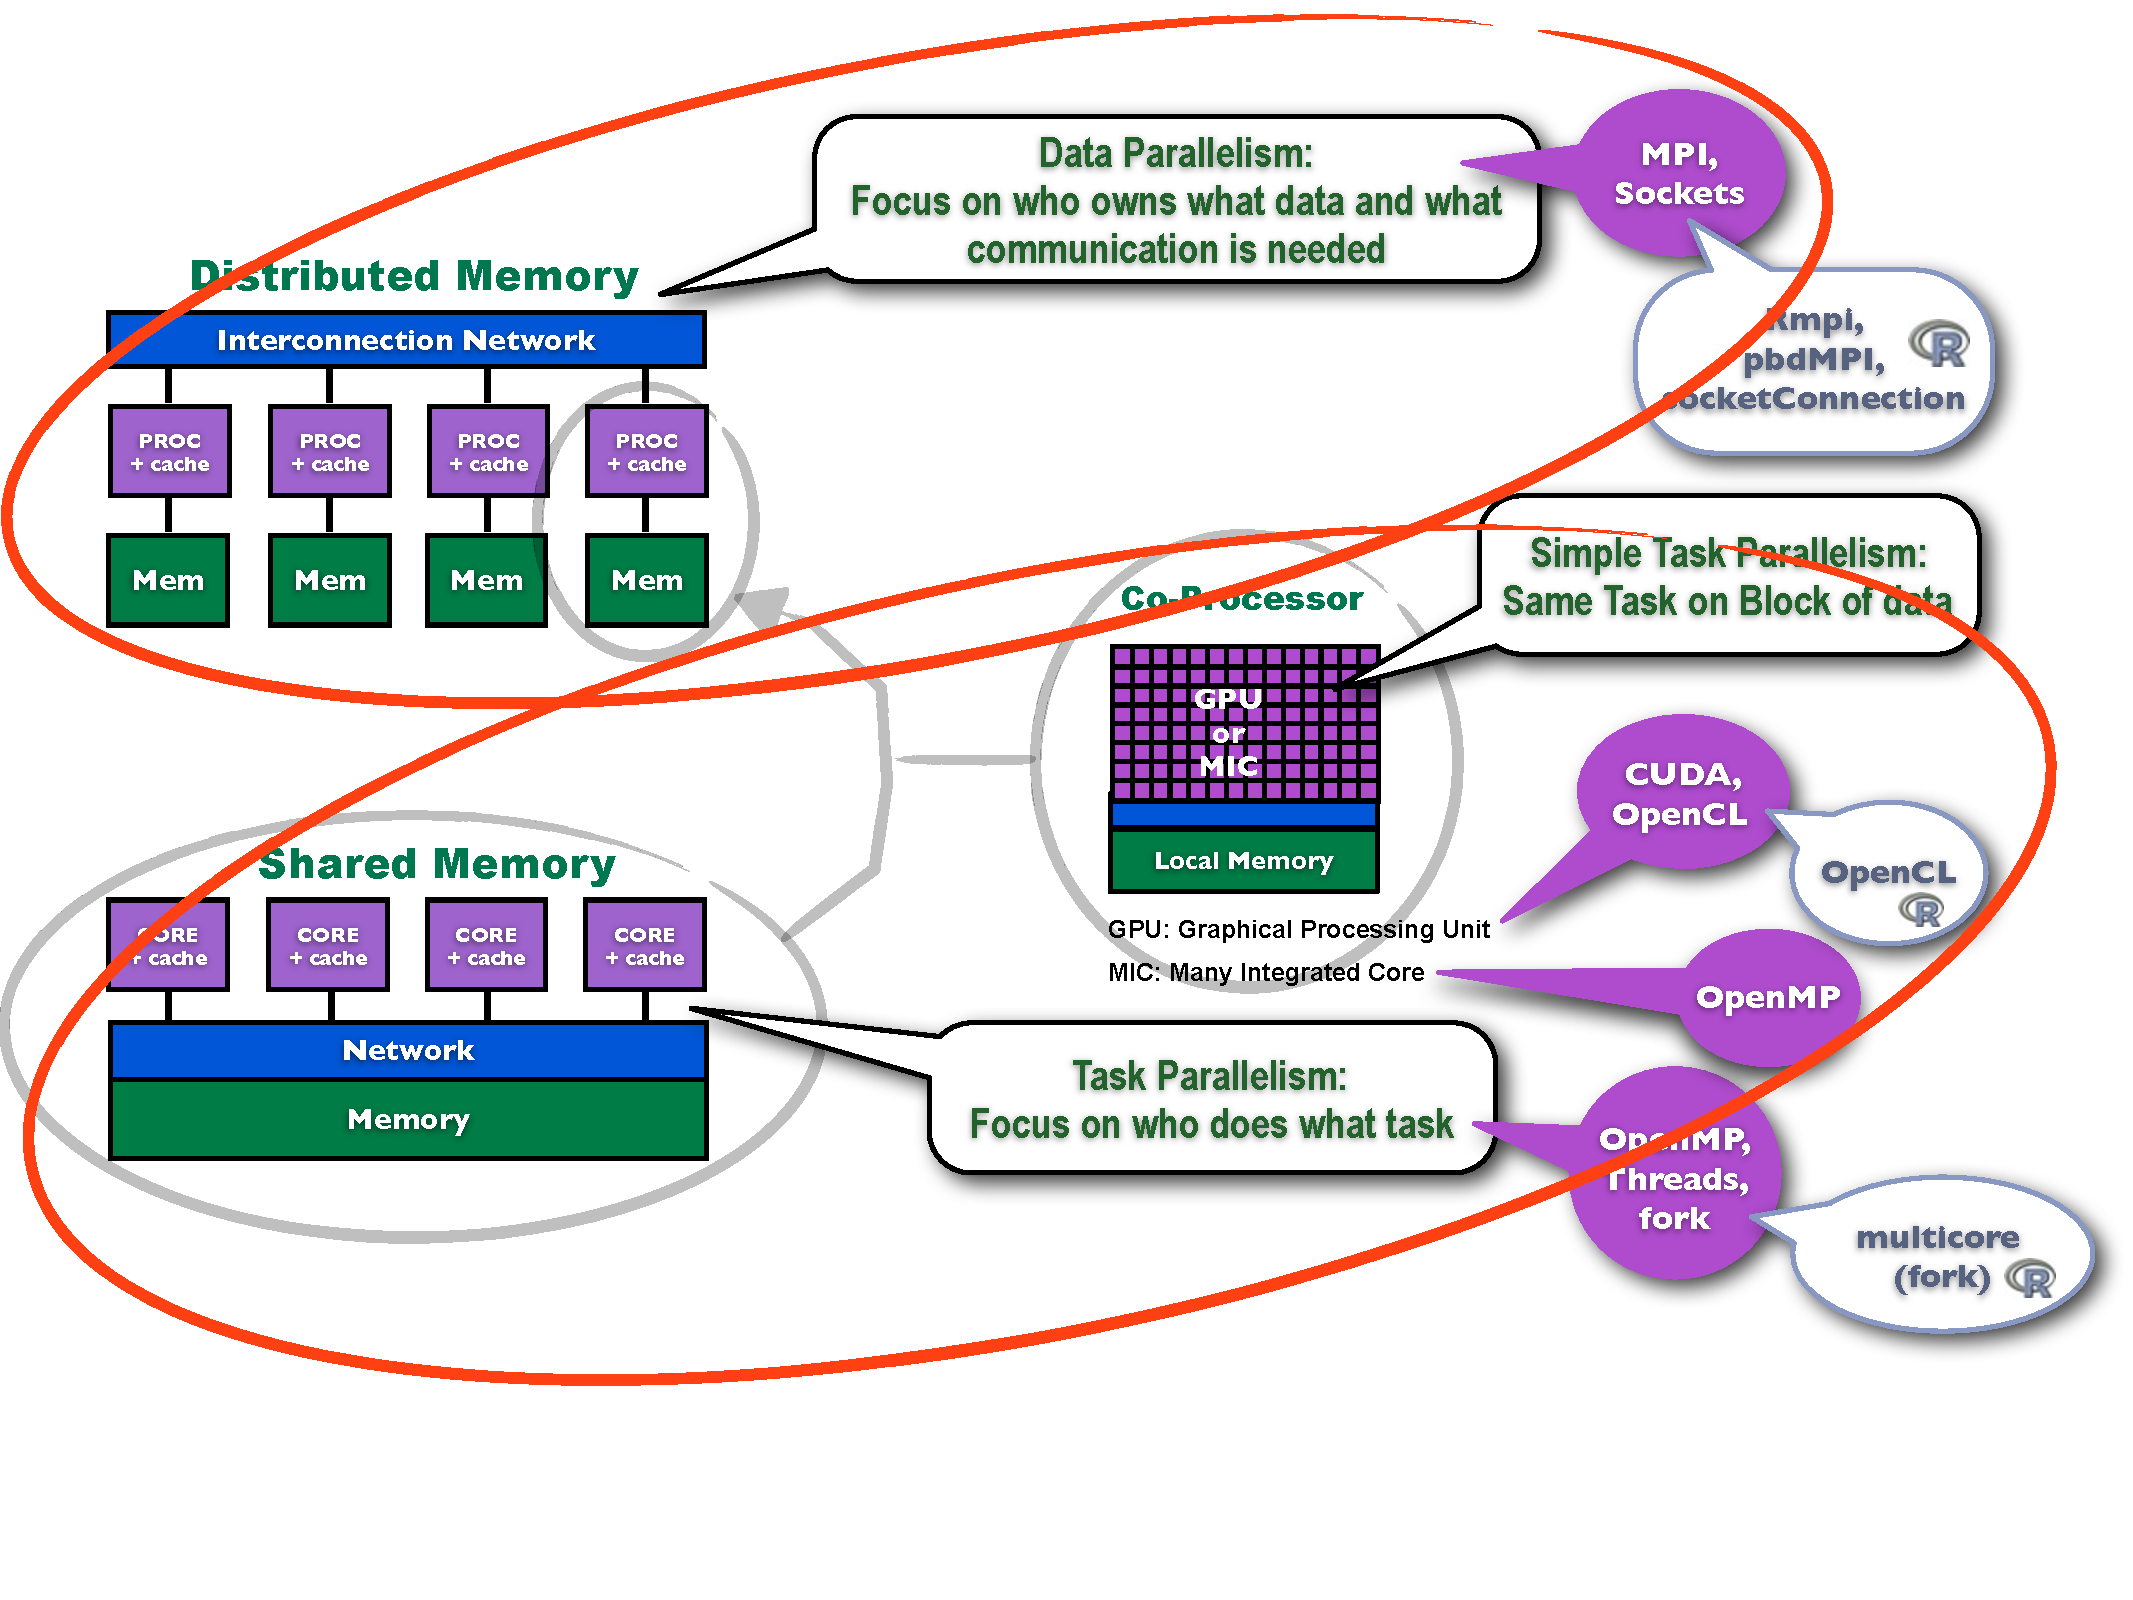
\includegraphics[width=0.95\textwidth]{../common/pics/ParallelHardware10.pdf}
\end{block}
\end{frame}

\begin{frame}
\begin{block}{pbdR Focus on Data Parallelism}
    
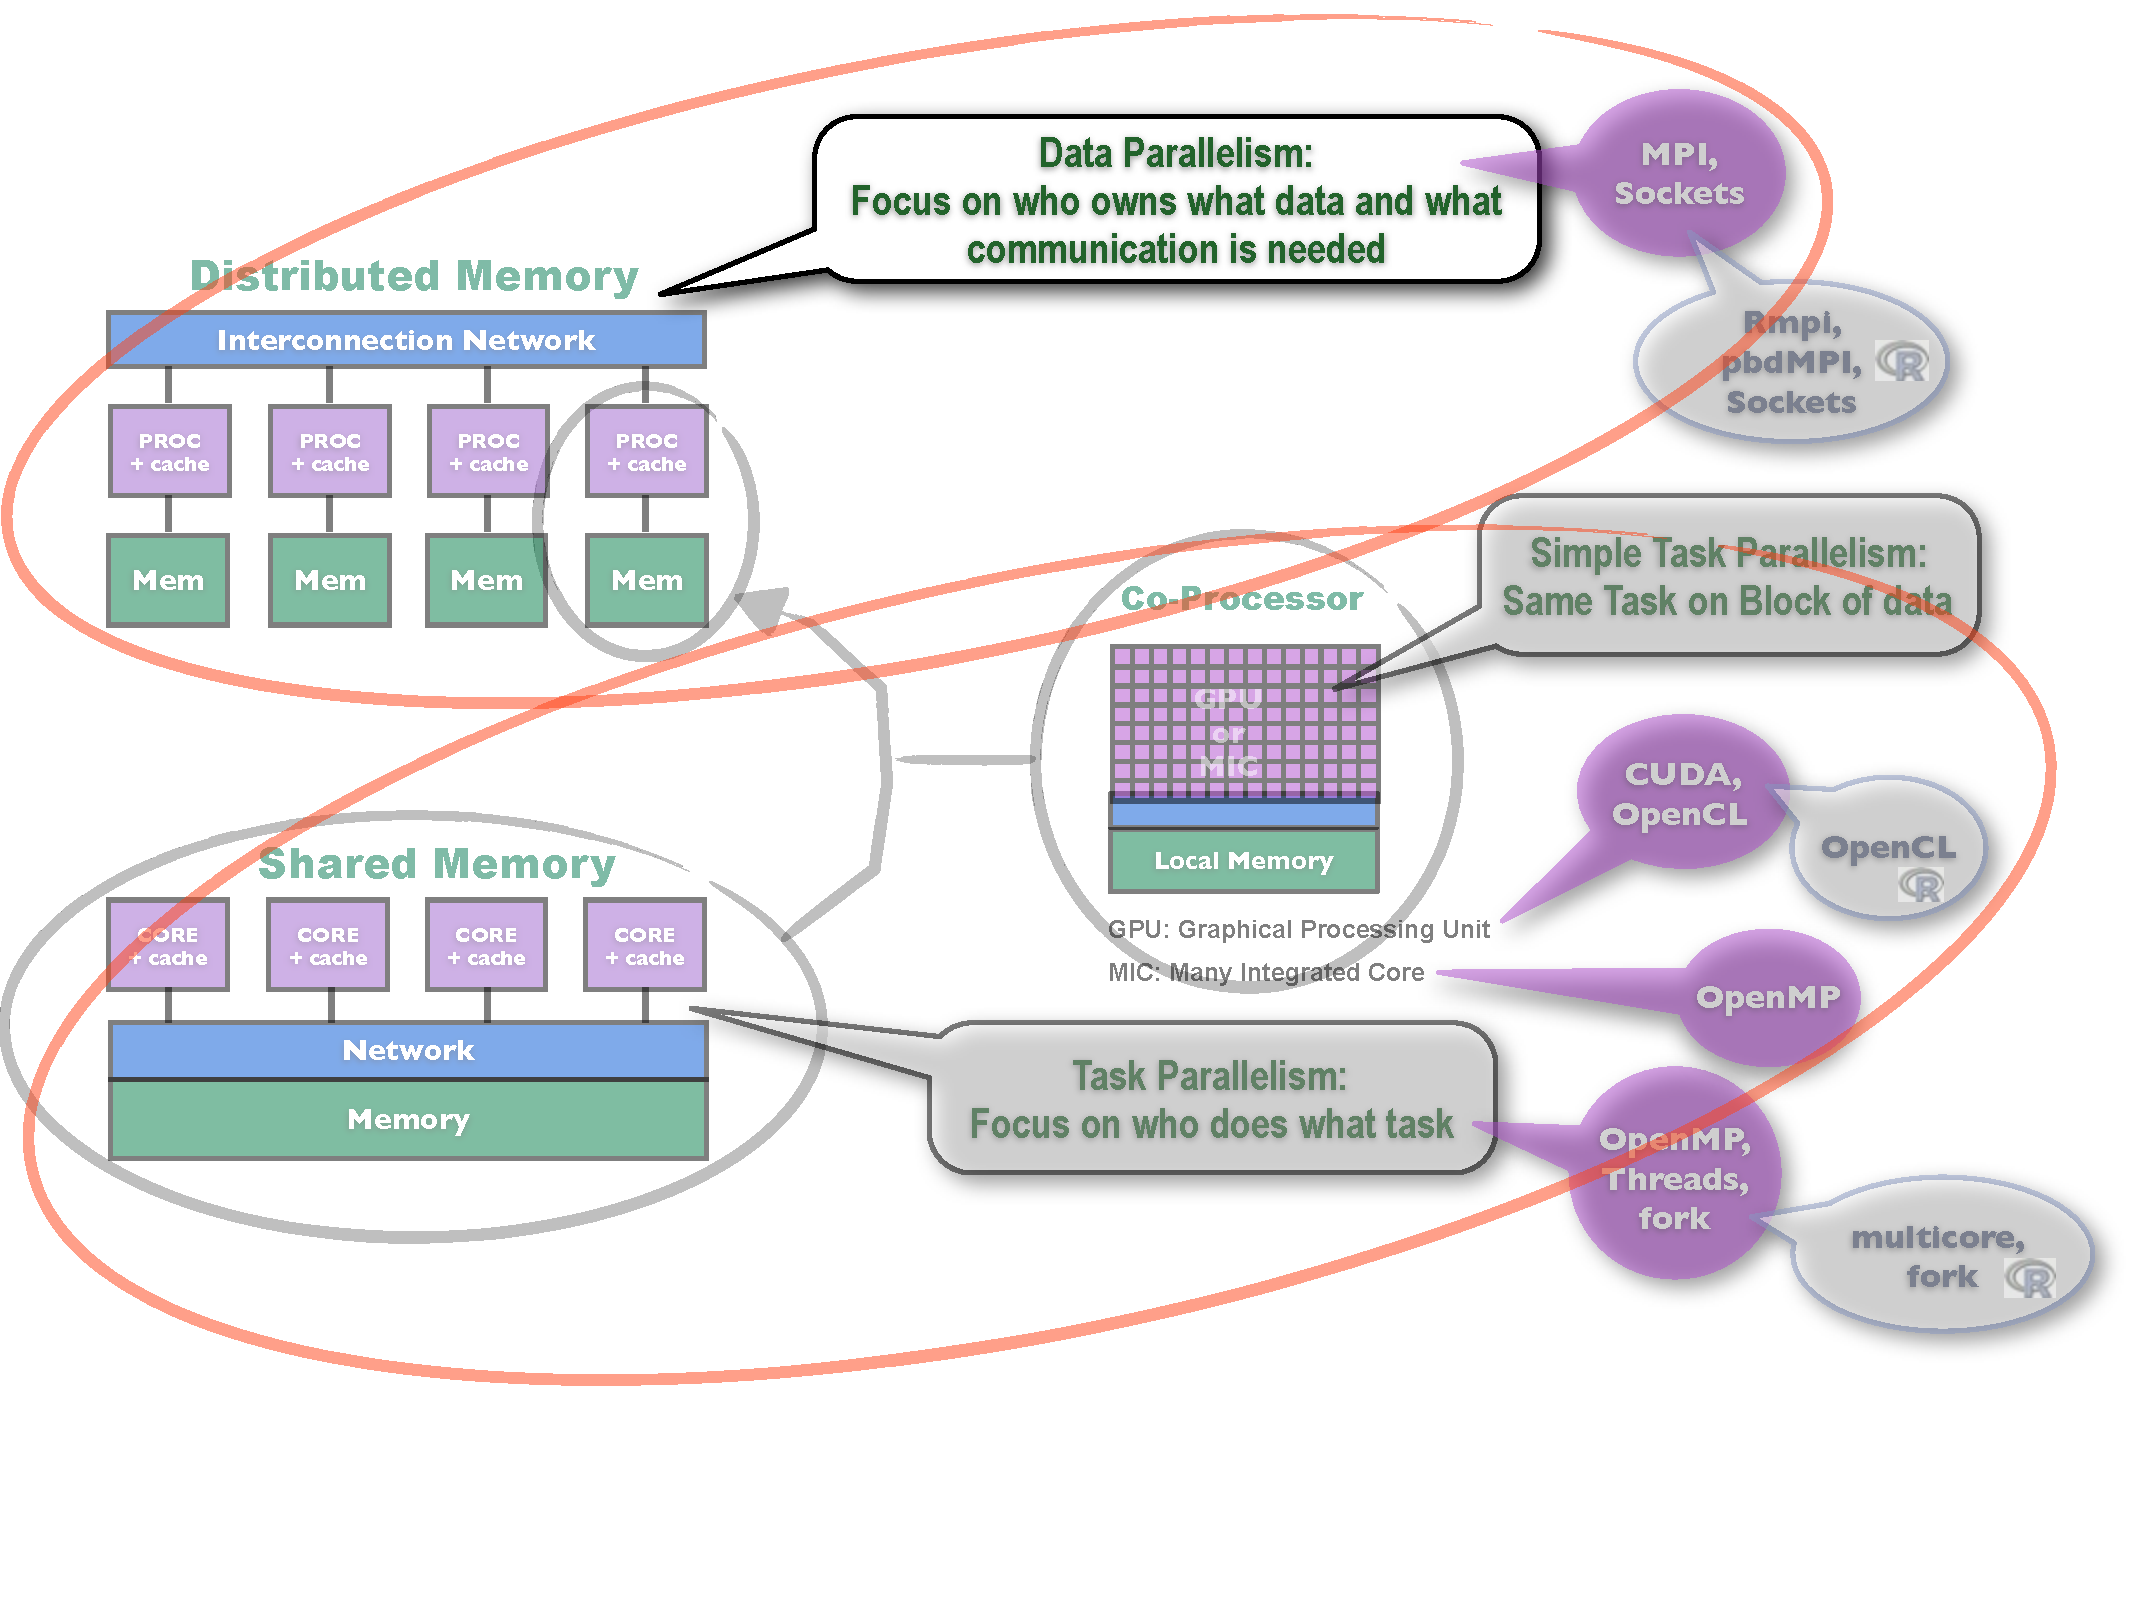
\includegraphics[width=0.95\textwidth]{../common/pics/ParallelHardware11.pdf}
\end{block}
\end{frame}

\section[Iris]{In-Depth Example Examining the Iris Dataset}

\hidenum
\begin{frame}[noframenumbering]
\frametitle{Contents}
 \tableofcontents[currentsection,hideothersubsections,sectionstyle=show/hide]
\end{frame}
\shownum

\subsection{Examining the Iris Dataset}

\begin{frame}[fragile]
  \begin{block}{The Iris Dataset}\pause
\begin{lstlisting}
rm(list = ls())                # Clean environment

head(iris)

### Load data
X <- as.matrix(iris[, -5])     # Dimension 150 by 4
X.cid <- as.numeric(iris[, 5]) # True id
\end{lstlisting}
\end{block}
\end{frame}


\begin{frame}[fragile]
  \begin{block}{Standardizing}\pause
\begin{lstlisting}
### Transformation and check
X.std <- scale(X)             # Standardize
mu <- colMeans(X.std)         # Columns means are near 0
cov <- cov(X.std)             # Diagonals are near 1
print(mu)
print(cov)
\end{lstlisting}
\end{block}
\end{frame}

\begin{frame}[fragile]
  \begin{block}{Projection Onto First 2 PC's}\pause
\begin{lstlisting}
### SVD
X.svd <- svd(X.std)

### Project on column space of singular vectors
A <- X.std %*% diag(X.svd$d)
B <- X.std %*% X.svd$v
C <- prcomp(X.std)$x            # A = B = C

X.prj <- C[, 1:2]               # project onto first 2 PC's
\end{lstlisting}
\end{block}
\end{frame}

\subsection{Cluster}

\begin{frame}[fragile]
  \begin{block}{Clustering}\pause
\begin{lstlisting}
### Clustering
set.seed(1234)                  # Set overall seed
X.kms <- kmeans(X.std, 3)       # K-means
X.kms
X.kms.cid <- X.kms$cluster      # Classification

library(EMCluster)              # Model-based clustering
X.mbc <- init.EM(X.std, 3)      # Initial by em-EM
X.mbc
X.mbc.cid <- X.mbc$class        # Classification
\end{lstlisting}
\end{block}
\end{frame}

\begin{frame}[fragile]
  \begin{block}{Cluster Validation}\pause
\begin{lstlisting}
### Validation
X.kms.adjR <- RRand(X.cid, X.kms.cid)$adjRand       # Adjusted Rand index
X.mbc.adjR <- RRand(X.cid, X.mbc.cid)$adjRand
\end{lstlisting}
\end{block}
\end{frame}

\begin{frame}[fragile]
  \begin{block}{Cluster ID Variable}\pause
\begin{lstlisting}
### Swap classification id
X.kms.cid[X.kms.cid == 2] <- 4
X.kms.cid[X.kms.cid == 3] <- 2
X.kms.cid[X.kms.cid == 4] <- 3
\end{lstlisting}
\end{block}
\end{frame}

\subsection{Plot}

\begin{frame}[fragile]
  \begin{block}{Plot}\pause
\begin{lstlisting}
### Display on first 2 components
pdf("serial_plot.pdf")

par(mfrow = c(2, 2))
plot(X.prj, col = X.cid + 1, pch = X.cid,
     main = "iris (true)", xlab = "PC1", ylab = "PC2")
plot(X.prj, col = X.kms.cid + 1, pch = X.kms.cid,
     main = paste("iris (k-Means)", sprintf("%.4f", X.kms.adjR)),
     xlab = "PC1", ylab = "PC2")
plot(X.prj, col = X.mbc.cid + 1, pch = X.mbc.cid,
     main = paste("iris (Model-based)", sprintf("%.4f", X.mbc.adjR)),
     xlab = "PC1", ylab = "PC2")
accuracy <- c(X.kms.adjR, X.mbc.adjR)
names(accuracy) <- c("k-Means", "Model-based")
barplot(accuracy, main = "Clustering Accuracy")

dev.off()
\end{lstlisting}
\end{block}
\end{frame}


\begin{frame}
  \begin{block}{Plot}\pause
\begin{center}
  \includegraphics[scale=.37]{other/serial_plot.pdf}
\end{center}
\end{block}
\end{frame}
\section{pbdR}

\hidenum
\begin{frame}[noframenumbering]
\frametitle{Contents}
 \tableofcontents[currentsection,hideothersubsections,sectionstyle=show/hide]
\end{frame}
\shownum

\subsection{Problems with R}

\begin{frame}
%  \addtocounter{framenumber}{-1}
  \begin{block}{Problems with R}\pause
  We \emph{love} R!  However\dots
  \begin{itemize}[<+-|alert@+>]
    \item Slow.
    \item If you don't know what you're doing, it's \emph{really} slow.
    \item Performance improvements usually for small machines.
    \item Very ram intensive.
    \item Chokes on big data.
  \end{itemize}
  \end{block}
\end{frame}

\begin{frame}
%  \addtocounter{framenumber}{-1}
  \begin{block}{Problems with R: Big Data}\pause
  One of R's biggest problems is an indexing limitation:
  \begin{itemize}[<+-|alert@+>]
    \item Any one R object must (at present) be indexed by a 32-bit integer.
    \item Largest vector/matrix:  16gb
    \item Largest square matrix:  $46340\times 46340$
  \end{itemize}
  \end{block}
\end{frame}

\begin{frame}[shrink]
  \begin{block}{R and Parallelism}
    The solution to many of R's problems is parallelism.  However \dots\vspace{-.4cm}
   \begin{center}
    \begin{minipage}[t]{.95\textwidth}
    \begin{block}{\centering What we have}
      \begin{enumerate}[<+-|alert@+>]
	\item Mostly serial.
	\item Parallelism mostly not distributed.
	\item Data parallelism mostly explicit.
      \end{enumerate}
    \end{block}
    \end{minipage}
    \\\pause
    \begin{minipage}[t]{.95\textwidth}
    \begin{block}{\centering What we want}
      \begin{enumerate}[<+-|alert@+>]
        \item Mostly parallel.
        \item Mostly distributed.
        \item Mostly implicit.
      \end{enumerate}
    \end{block}
    \end{minipage}
    \end{center}
    \end{block}
\end{frame}


\subsection{The pbdR Project}

\begin{frame}[squeeze]
  \begin{block}{Programming with Big Data in R (pbdR)}\pause
  Goals:  \emph{Productivity, Portability, Performance}\\[.4cm]\pause
  Our Approach:
  \begin{itemize}[<+-|alert@+>]
    \item Series of \emph{free}\footnote{MPL, BSD, and GPL licensed} R packages.
    \item Scalable, big data analytics with high-level syntax.
    \item Implicit management of distributed data details.
    \item Methods have syntax \emph{identical} to R.
    \item Powered by state of the art numerical libraries (MPI, ScaLAPACK, PBLAS, BLACS, LAPACK, BLAS, \dots)
  \end{itemize}
  \end{block}
\end{frame}

\begin{frame}[shrink]
  \begin{block}{pbdR Packages}
    \begin{center}
	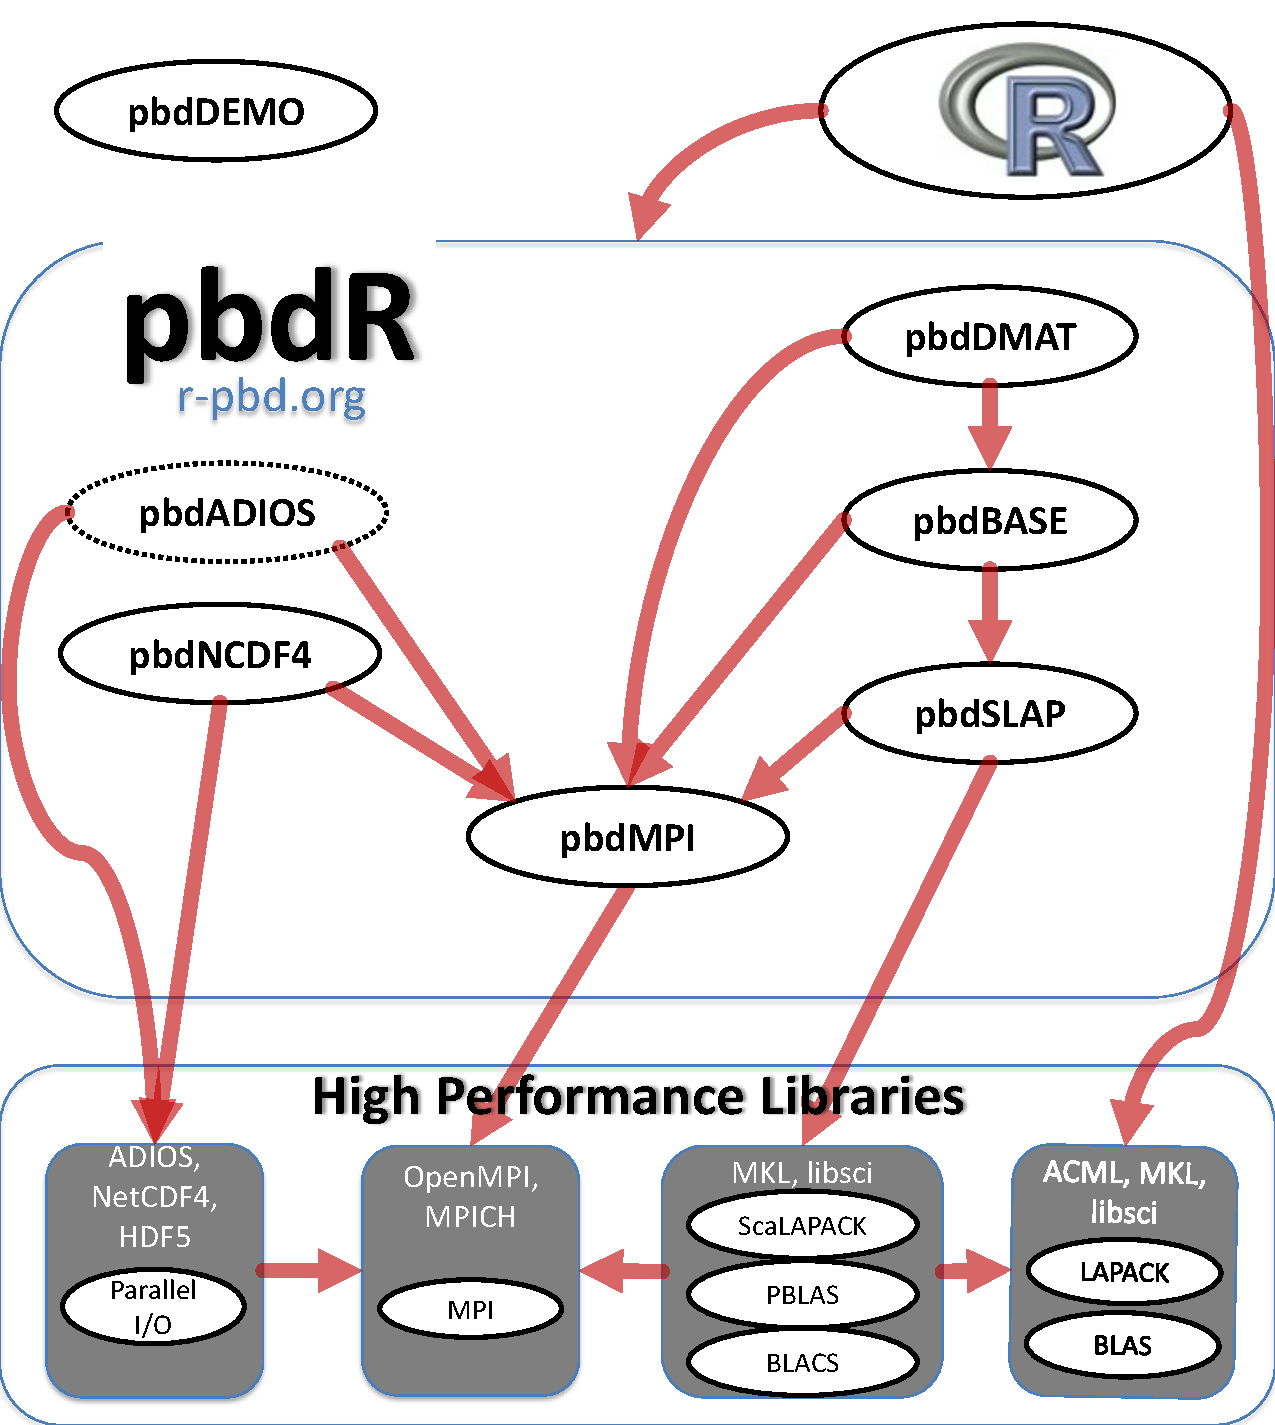
\includegraphics[width=7cm, height=7cm]{pics/pbdpacks}
    \end{center}
  \end{block}
\end{frame}


\begin{frame}[shrink]
  \begin{block}{pbdR Packages --- http://code.r-pbd.org}\pause
  Released to CRAN:
  \begin{itemize}[<+-|alert@+>]
    \item \pkg{pbdMPI}: MPI bindings (explicit, low-level)
    \item \pkg{pbdSLAP}: Foreign library (just install it, nothing to use)
    \item \pkg{pbdBASE}: Compiled code (used by DMAT, also for devs)
    \item \pkg{pbdDMAT}: Distributed matrices (mostly implicit, high-level)
    \item \pkg{pbdNCDF4}: Parallel NetCDF4 reader
    \item \pkg{pbdDEMO}: Package demonstrations, examples, vignette written in textbook style
  \end{itemize}
%     \\[.2cm]
    Future Development:
  \begin{itemize}[<+-|alert@+>]
    \item \pkg{pbdADIOS}: Wrappers for ADIOS middleware
    \item Profiling tools
    \item Client/server interface for interactive sessions
    \item Something for you\dots?
  \end{itemize}
  \end{block}
\end{frame}

\begin{frame}
  \begin{block}{SPMD}\pause
  The pbdR Packages enable high-level ``Single Program/Multiple Data'' (SPMD) programming:
    \begin{itemize}
      \item SPMD is a programming \emph{paradigm}.
      \item Arguably the simplest extension of serial programming.
      \item Sort of like trying to explain breathing \dots
      \item Not to be confused with SIMD.
      \item SPMD utilizes MIMD architecture computers.
      \item Only one program is written, executed in batch independently on all processors.
      \item Different processors are autonomous; there is no manager.
%       \item Like ``Map/Reduce'', you probably used it without knowing it even had a name.
    \end{itemize}
  \end{block}
\end{frame}


\begin{frame}[fragile]
  \begin{block}{SPMD}\pause
      SPMD codes are run in batch (non-interactively):
\begin{lstlisting}[backgroundcolor=\color{white},keywordstyle=\color{black},title=From the Shell]
mpirun -np 4 Rscript my_script.R
\end{lstlisting}
  \end{block}
\end{frame}


\begin{frame}[fragile]
  \begin{block}{Example Syntax}\pause
  \begin{lstlisting}
x <- x[-1, 2:5]
xtx <- t(x) %*% x
ans <- svd(solve(xtx))
  \end{lstlisting}
  \begin{center}
  \pause Look familiar?\\[.4cm] \pause
  \emph{The above runs on 1 core with R or 10,000 cores with pbdR}
  \end{center}
  \end{block}
\end{frame}



\subsection{Installing pbdR}

\begin{frame}[fragile]
  \begin{block}{Installation}\pause
  Installing pbdR is about as easy as possible, and generally amounts to:
  \begin{lstlisting}
install.packages(pbdMPI)
install.packages(pbdNCDF4)
install.packages(pbdSLAP)
install.packages(pbdBASE)
install.packages(pbdDMAT)
install.packages(pbdDEMO)
  \end{lstlisting}
  But this assumes you have MPI installed on your system\dots
  \end{block}
\end{frame}


\begin{frame}[fragile]
  \begin{block}{NICS Allocation}\pause
  Instead, consider getting an allocation on Nautilus:
  \begin{center}
  \url{http://www.nics.tennessee.edu/getting-an-allocation}\\
  
\includegraphics[scale=.3]{pics/nics}
  \end{center}
  \end{block}
\end{frame}
\section[Break]{Brief Intermission}
\hidenum
\begin{frame}[noframenumbering]
\frametitle{Brief Intermission}
  \begin{block}{Brief Intermission}
  \begin{center}
     {\Large Questions?  Comments?}\\[.4cm]
     Don't forget to talk to us at our discussion group: \url{http://group.r-pbd.org/}\\[.4cm]
     Don't have an allocation with us?  \\
     \url{http://www.nics.tennessee.edu/getting-an-allocation}
  \end{center}
  \end{block}
\end{frame}
\shownum


\section[GBD]{The Generalized Block Distribution}

\hidenum
\begin{frame}[noframenumbering]
\frametitle{Contents}
 \tableofcontents[currentsection,hideothersubsections,sectionstyle=show/hide]
\end{frame}
\shownum


\subsection{The GBD Data Structure}


\begin{frame}
  \begin{block}{Distributing Data}
  \centering
\textbf{Problem:}  How to distribute the data
\begin{center}
    \begin{minipage}{0.47\textwidth}
     \begin{center}
      \begin{align*}
      x &= \left[
            \begin{array}{lll}
            x_{1,1} & x_{1,2} & x_{1,3} \\
            x_{2,1} & x_{2,2} & x_{2,3} \\
            x_{3,1} & x_{3,2} & x_{3,3} \\
            x_{4,1} & x_{4,2} & x_{4,3} \\
            x_{5,1} & x_{5,2} & x_{5,3} \\
            x_{6,1} & x_{6,2} & x_{6,3} \\
            x_{7,1} & x_{7,2} & x_{7,3} \\
            x_{8,1} & x_{8,2} & x_{8,3} \\
            x_{9,1} & x_{9,2} & x_{9,3} \\
            x_{10,1} & x_{10,2} & x_{10,3} \\
            \end{array}
      \right]_{10\times 3}
      \end{align*}
     \end{center}
    \end{minipage}
    \begin{minipage}{0.47\textwidth}
    \centering
      {\fontsize{12cm}{1cm}\selectfont ? }
    \end{minipage}
    \end{center}
  \end{block}
\end{frame}



\begin{frame}
\begin{exampleblock}{Distributing a Matrix Across 4 Processors: Block Distribution}
  \begin{columns}[t,onlytextwidth]
    \begin{column}{0.5\textwidth}
      \hfill Data \hfill\ 
      \begin{align*}
      x &= \left[
            \begin{array}{lll}
            \color{g11}x_{1,1} & \color{g11}x_{1,2} & \color{g11}x_{1,3} \\
            \color{g11}x_{2,1} & \color{g11}x_{2,2} & \color{g11}x_{2,3} \\
            \color{g11}x_{3,1} & \color{g11}x_{3,2} & \color{g11}x_{3,3} \\\hline
            \color{g12}x_{4,1} & \color{g12}x_{4,2} & \color{g12}x_{4,3} \\
            \color{g12}x_{5,1} & \color{g12}x_{5,2} & \color{g12}x_{5,3} \\
            \color{g12}x_{6,1} & \color{g12}x_{6,2} & \color{g12}x_{6,3} \\\hline
            \color{g13}x_{7,1} & \color{g13}x_{7,2} & \color{g13}x_{7,3} \\
            \color{g13}x_{8,1} & \color{g13}x_{8,2} & \color{g13}x_{8,3} \\
            \color{g13}x_{9,1} & \color{g13}x_{9,2} & \color{g13}x_{9,3} \\\hline
            \color{g21}x_{10,1} & \color{g21}x_{10,2} & \color{g21}x_{10,3} \\
            \end{array}
      \right]_{10\times 3}
      \end{align*}
    \end{column}
    \begin{column}{0.5\textwidth}
    \hfill Processors \hfill\ 
      \begin{align*}
      \begin{tabular}{l}
        \color{g11}0 \\
        \color{g12}1 \\
        \color{g13}2 \\
        \color{g21}3 
      \end{tabular}
      \end{align*}
    \end{column}
  \end{columns}
\end{exampleblock}
\end{frame}


\begin{frame}
\begin{exampleblock}{Distributing a Matrix Across 4 Processors: Local Load Balance}
  \begin{columns}[t,onlytextwidth]
    \begin{column}{0.5\textwidth}
      \hfill Data \hfill\ 
      \begin{align*}
      x &= \left[
            \begin{array}{lll}
            \color{g11}x_{1,1} & \color{g11}x_{1,2} & \color{g11}x_{1,3} \\
            \color{g11}x_{2,1} & \color{g11}x_{2,2} & \color{g11}x_{2,3} \\
            \color{g11}x_{3,1} & \color{g11}x_{3,2} & \color{g11}x_{3,3} \\\hline
            \color{g12}x_{4,1} & \color{g12}x_{4,2} & \color{g12}x_{4,3} \\
            \color{g12}x_{5,1} & \color{g12}x_{5,2} & \color{g12}x_{5,3} \\
            \color{g12}x_{6,1} & \color{g12}x_{6,2} & \color{g12}x_{6,3} \\\hline
            \color{g13}x_{7,1} & \color{g13}x_{7,2} & \color{g13}x_{7,3} \\
            \color{g13}x_{8,1} & \color{g13}x_{8,2} & \color{g13}x_{8,3} \\\hline
            \color{g21}x_{9,1} & \color{g21}x_{9,2} & \color{g21}x_{9,3} \\
            \color{g21}x_{10,1} & \color{g21}x_{10,2} & \color{g21}x_{10,3} \\
            \end{array}
      \right]_{10\times 3}
      \end{align*}
    \end{column}
    \begin{column}{0.5\textwidth}
    \hfill Processors \hfill\ 
      \begin{align*}
      \begin{tabular}{l}
        \color{g11}0 \\
        \color{g12}1 \\
        \color{g13}2 \\
        \color{g21}3 
      \end{tabular}
      \end{align*}
    \end{column}
  \end{columns}
\end{exampleblock}
\end{frame}




\begin{frame}[fragile]
  \fontsize{8pt}{10}\selectfont
  \begin{block}{The \code{GBD} Data Structure}\pause
  Throughout the examples, we will make use of the Generalized Block Distribution, or \code{GBD} distributed matrix structure.
  \begin{columns}[c,onlytextwidth]
    \begin{column}{0.64\textwidth}
  \begin{enumerate}
    \item \code{GBD} is \emph{distributed}.  No processor owns all the data.
    \item \code{GBD} is \emph{non-overlapping}. Rows uniquely assigned to processors.
    \item \code{GBD} is \emph{row-contiguous}.  If a processor owns one element of a row, it owns the entire row.
    \item \code{GBD} is globally \emph{row-major}, locally \emph{column-major}.
    \item \code{GBD} is often \emph{locally balanced}, where each processor owns (almost) the same amount of data.  But this is not required.
    \end{enumerate}
    \end{column}
    \begin{column}{0.35\textwidth}
      \begin{align*}
      \left[
            \begin{array}{lll}
            \color{g11}x_{1,1} & \color{g11}x_{1,2} & \color{g11}x_{1,3} \\
            \color{g11}x_{2,1} & \color{g11}x_{2,2} & \color{g11}x_{2,3} \\
            \color{g11}x_{3,1} & \color{g11}x_{3,2} & \color{g11}x_{3,3} \\\hline
            \color{g12}x_{4,1} & \color{g12}x_{4,2} & \color{g12}x_{4,3} \\
            \color{g12}x_{5,1} & \color{g12}x_{5,2} & \color{g12}x_{5,3} \\
            \color{g12}x_{6,1} & \color{g12}x_{6,2} & \color{g12}x_{6,3} \\\hline
            \color{g13}x_{7,1} & \color{g13}x_{7,2} & \color{g13}x_{7,3} \\
            \color{g13}x_{8,1} & \color{g13}x_{8,2} & \color{g13}x_{8,3} \\\hline
            \color{g21}x_{9,1} & \color{g21}x_{9,2} & \color{g21}x_{9,3} \\\
            \color{g21}x_{10,1} & \color{g21}x_{10,2} & \color{g21}x_{10,3} \\
            \end{array}
      \right]
      \end{align*}
    \end{column}
  \end{columns}
  \begin{enumerate}
    \setcounter{enumi}{5}
    \item The last row of the local storage of a processor is adjacent (by global row) to the first row of the local storage of next processor (by communicator number) that owns data.
    \item \code{GBD} is (relatively) easy to understand, but can lead to bottlenecks if you have many more columns than rows.
  \end{enumerate}
  \end{block}
\end{frame}





\subsection{GBD:  Example 1}

\begin{frame}
\begin{exampleblock}{Understanding GBD:  Global Matrix}
\begin{align*}
x &= \left[
      \begin{array}{lllllllll}
      x_{11} & x_{12} & x_{13} & x_{14} & x_{15} & x_{16} & x_{17} & x	_{18} & x_{19}\\
      x_{21} & x_{22} & x_{23} & x_{24} & x_{25} & x_{26} & x_{27} & x	_{28} & x_{29}\\
      x_{31} & x_{32} & x_{33} & x_{34} & x_{35} & x_{36} & x_{37} & x	_{38} & x_{39}\\
      x_{41} & x_{42} & x_{43} & x_{44} & x_{45} & x_{46} & x_{47} & x	_{48} & x_{49}\\
      x_{51} & x_{52} & x_{53} & x_{54} & x_{55} & x_{56} & x_{57} & x	_{58} & x_{59}\\
      x_{61} & x_{62} & x_{63} & x_{64} & x_{65} & x_{66} & x_{67} & x	_{68} & x_{69}\\
      x_{71} & x_{72} & x_{73} & x_{74} & x_{75} & x_{76} & x_{77} & x	_{78} & x_{79}\\
      x_{81} & x_{82} & x_{83} & x_{84} & x_{85} & x_{86} & x_{87} & x	_{88} & x_{89}\\
      x_{91} & x_{92} & x_{93} & x_{94} & x_{95} & x_{96} & x_{97} & x	_{98} & x_{99}
      \end{array}
\right]_{9\times 9}
\end{align*}
\begin{align*}
\text{Processors = }
      \begin{array}{llllll}
      \color{g11}0 & \color{g12}1 & \color{g13}2 & \color{g21}3 & \color{g22}4 & \color{g23}5
      \end{array}
\end{align*}
\end{exampleblock}
\end{frame}


\begin{frame}
\begin{exampleblock}{Understanding GBD:  Load Balanced GBD}
\begin{align*}
x &= \left[
      \begin{array}{lllllllll}
      \color{g11}x_{11} & \color{g11}x_{12} & \color{g11}x_{13} & \color{g11}x_{14} & \color{g11}x_{15} & \color{g11}x_{16} & \color{g11}x_{17} & \color{g11}x_{18} & \color{g11}x_{19}\\
      %
      \color{g11}x_{21} & \color{g11}x_{22} & \color{g11}x_{23} & \color{g11}x_{24} & \color{g11}x_{25} & \color{g11}x_{26} & \color{g11}x_{27} & \color{g11}x_{28} & \color{g11}x_{29}\\\hline
      %
      \color{g12}x_{31} & \color{g12}x_{32} & \color{g12}x_{33} & \color{g12}x_{34} & \color{g12}x_{35} & \color{g12}x_{36} & \color{g12}x_{37} & \color{g12}x_{38} & \color{g12}x_{39}\\
      %
      \color{g12}x_{41} & \color{g12}x_{42} & \color{g12}x_{43} & \color{g12}x_{44} & \color{g12}x_{45} & \color{g12}x_{46} & \color{g12}x_{47} & \color{g12}x_{48} & \color{g12}x_{49}\\\hline
      %
      \color{g13}x_{51} & \color{g13}x_{52} & \color{g13}x_{53} & \color{g13}x_{54} & \color{g13}x_{55} & \color{g13}x_{56} & \color{g13}x_{57} & \color{g13}x_{58} & \color{g13}x_{59}\\
      %
      \color{g13}x_{61} & \color{g13}x_{62} & \color{g13}x_{63} & \color{g13}x_{64} & \color{g13}x_{65} & \color{g13}x_{66} & \color{g13}x_{67} & \color{g13}x_{68} & \color{g13}x_{69}\\\hline
      %
      \color{g21}x_{71} & \color{g21}x_{72} & \color{g21}x_{73} & \color{g21}x_{74} & \color{g21}x_{75} & \color{g21}x_{76} & \color{g21}x_{77} & \color{g21}x_{78} & \color{g21}x_{79}\\\hline
      %
      \color{g22}x_{81} & \color{g22}x_{82} & \color{g22}x_{83} & \color{g22}x_{84} & \color{g22}x_{85} & \color{g22}x_{86} & \color{g22}x_{87} & \color{g22}x_{88} & \color{g22}x_{89}\\\hline
      %
      \color{g23}x_{91} & \color{g23}x_{92} & \color{g23}x_{93} & \color{g23}x_{94} & \color{g23}x_{95} & \color{g23}x_{96} & \color{g23}x_{97} & \color{g23}x_{98} & \color{g23}x_{99}\\
      \end{array}
\right]_{9\times 9}
\end{align*}
\begin{align*}
\text{Processors = }
      \begin{array}{llllll}
      \color{g11}0 & \color{g12}1 & \color{g13}2 & \color{g21}3 & \color{g22}4 & \color{g23}5
      \end{array}
\end{align*}
\end{exampleblock}
\end{frame}

\begin{frame}[shrink]
\begin{exampleblock}{Understanding GBD:  Local View}
\begin{align*}
\left[\begin{array}{lllllllll}
      \color{g11}x_{11} & \color{g11}x_{12} & \color{g11}x_{13} & \color{g11}x_{14} & \color{g11}x_{15} & \color{g11}x_{16} & \color{g11}x_{17} & \color{g11}x_{18} & \color{g11}x_{19}\\
      \color{g11}x_{21} & \color{g11}x_{22} & \color{g11}x_{23} & \color{g11}x_{24} & \color{g11}x_{25} & \color{g11}x_{26} & \color{g11}x_{27} & \color{g11}x_{28} & \color{g11}x_{29}
\end{array}\right]_{2\times 9}
\\
\left[\begin{array}{lllllllll}
      \color{g12}x_{31} & \color{g12}x_{32} & \color{g12}x_{33} & \color{g12}x_{34} & \color{g12}x_{35} & \color{g12}x_{36} & \color{g12}x_{37} & \color{g12}x_{38} & \color{g12}x_{39}\\
      \color{g12}x_{41} & \color{g12}x_{42} & \color{g12}x_{43} & \color{g12}x_{44} & \color{g12}x_{45} & \color{g12}x_{46} & \color{g12}x_{47} & \color{g12}x_{48} & \color{g12}x_{49}
\end{array}\right]_{2\times 9}
\\
\left[\begin{array}{lllllllll}
      \color{g13}x_{51} & \color{g13}x_{52} & \color{g13}x_{53} & \color{g13}x_{54} & \color{g13}x_{55} & \color{g13}x_{56} & \color{g13}x_{57} & \color{g13}x_{58} & \color{g13}x_{59}\\
      \color{g13}x_{61} & \color{g13}x_{62} & \color{g13}x_{63} & \color{g13}x_{64} & \color{g13}x_{65} & \color{g13}x_{66} & \color{g13}x_{67} & \color{g13}x_{68} & \color{g13}x_{69}
\end{array}\right]_{2\times 9}
\\
\left[\begin{array}{lllllllll}
      \color{g21}x_{71} & \color{g21}x_{72} & \color{g21}x_{73} & \color{g21}x_{74} & \color{g21}x_{75} & \color{g21}x_{76} & \color{g21}x_{77} & \color{g21}x_{78} & \color{g21}x_{79}
\end{array}\right]_{1\times 9}
\\
\left[\begin{array}{lllllllll}
      \color{g22}x_{81} & \color{g22}x_{82} & \color{g22}x_{83} & \color{g22}x_{84} & \color{g22}x_{85} & \color{g22}x_{86} & \color{g22}x_{87} & \color{g22}x_{88} & \color{g22}x_{89}
\end{array}\right]_{1\times 9}
\\
\left[\begin{array}{lllllllll}
      \color{g23}x_{91} & \color{g23}x_{92} & \color{g23}x_{93} & \color{g23}x_{94} & \color{g23}x_{95} & \color{g23}x_{96} & \color{g23}x_{97} & \color{g23}x_{98} & \color{g23}x_{99}\\
\end{array}\right]_{1\times 9}
\end{align*}
\begin{align*}
\text{Processors = }
      \begin{array}{llllll}
      \color{g11}0 & \color{g12}1 & \color{g13}2 & \color{g21}3 & \color{g22}4 & \color{g23}5
      \end{array}
\end{align*}
\end{exampleblock}
\end{frame}



\subsection{GBD:  Example 2}

\begin{frame}
\begin{exampleblock}{Understanding GBD:  Non-Balanced GBD}
\begin{align*}
x &= \left[
      \begin{array}{lllllllll}
      \\\hline
      \color{g12}x_{11} & \color{g12}x_{12} & \color{g12}x_{13} & \color{g12}x_{14} & \color{g12}x_{15} & \color{g12}x_{16} & \color{g12}x_{17} & \color{g12}x_{18} & \color{g12}x_{19}\\
      %
      \color{g12}x_{21} & \color{g12}x_{22} & \color{g12}x_{23} & \color{g12}x_{24} & \color{g12}x_{25} & \color{g12}x_{26} & \color{g12}x_{27} & \color{g12}x_{28} & \color{g12}x_{29}\\
      %
      \color{g12}x_{31} & \color{g12}x_{32} & \color{g12}x_{33} & \color{g12}x_{34} & \color{g12}x_{35} & \color{g12}x_{36} & \color{g12}x_{37} & \color{g12}x_{38} & \color{g12}x_{39}\\
      %
      \color{g12}x_{41} & \color{g12}x_{42} & \color{g12}x_{43} & \color{g12}x_{44} & \color{g12}x_{45} & \color{g12}x_{46} & \color{g12}x_{47} & \color{g12}x_{48} & \color{g12}x_{49}\\\hline
      %%%%
      \color{g13}x_{51} & \color{g13}x_{52} & \color{g13}x_{53} & \color{g13}x_{54} & \color{g13}x_{55} & \color{g13}x_{56} & \color{g13}x_{57} & \color{g13}x_{58} & \color{g13}x_{59}\\
      %
      \color{g13}x_{61} & \color{g13}x_{62} & \color{g13}x_{63} & \color{g13}x_{64} & \color{g13}x_{65} & \color{g13}x_{66} & \color{g13}x_{67} & \color{g13}x_{68} & \color{g13}x_{69}\\\hline
      %%%%
      \color{g21}x_{71} & \color{g21}x_{72} & \color{g21}x_{73} & \color{g21}x_{74} & \color{g21}x_{75} & \color{g21}x_{76} & \color{g21}x_{77} & \color{g21}x_{78} & \color{g21}x_{79}\\\hline\hline
      %%%%
      \color{g23}x_{81} & \color{g23}x_{82} & \color{g23}x_{83} & \color{g23}x_{84} & \color{g23}x_{85} & \color{g23}x_{86} & \color{g23}x_{87} & \color{g23}x_{88} & \color{g23}x_{89}\\
      %
      \color{g23}x_{91} & \color{g23}x_{92} & \color{g23}x_{93} & \color{g23}x_{94} & \color{g23}x_{95} & \color{g23}x_{96} & \color{g23}x_{97} & \color{g23}x_{98} & \color{g23}x_{99}\\
      \end{array}
\right]_{9\times 9}
\end{align*}
\begin{align*}
\text{Processors = }
      \begin{array}{llllll}
      \color{g11}0 & \color{g12}1 & \color{g13}2 & \color{g21}3 & \color{g22}4 & \color{g23}5
      \end{array}
\end{align*}
\end{exampleblock}
\end{frame}

\begin{frame}[shrink]
\begin{exampleblock}{Understanding GBD:  Local View}
\begin{align*}
\left[\begin{array}{lllllllll}
      &&&&&&&&\hspace{4.55cm} 
\end{array}\right]_{0\times 9}
\\
\left[\begin{array}{lllllllll}
      \color{g12}x_{11} & \color{g12}x_{12} & \color{g12}x_{13} & \color{g12}x_{14} & \color{g12}x_{15} & \color{g12}x_{16} & \color{g12}x_{17} & \color{g12}x_{18} & \color{g12}x_{19}\\
      %
      \color{g12}x_{21} & \color{g12}x_{22} & \color{g12}x_{23} & \color{g12}x_{24} & \color{g12}x_{25} & \color{g12}x_{26} & \color{g12}x_{27} & \color{g12}x_{28} & \color{g12}x_{29}\\
      %
      \color{g12}x_{31} & \color{g12}x_{32} & \color{g12}x_{33} & \color{g12}x_{34} & \color{g12}x_{35} & \color{g12}x_{36} & \color{g12}x_{37} & \color{g12}x_{38} & \color{g12}x_{39}\\
      %
      \color{g12}x_{41} & \color{g12}x_{42} & \color{g12}x_{43} & \color{g12}x_{44} & \color{g12}x_{45} & \color{g12}x_{46} & \color{g12}x_{47} & \color{g12}x_{48} & \color{g12}x_{49}\\
\end{array}\right]_{4\times 9}
\\
\left[\begin{array}{lllllllll}
      \color{g13}x_{51} & \color{g13}x_{52} & \color{g13}x_{53} & \color{g13}x_{54} & \color{g13}x_{55} & \color{g13}x_{56} & \color{g13}x_{57} & \color{g13}x_{58} & \color{g13}x_{59}\\
      %
      \color{g13}x_{61} & \color{g13}x_{62} & \color{g13}x_{63} & \color{g13}x_{64} & \color{g13}x_{65} & \color{g13}x_{66} & \color{g13}x_{67} & \color{g13}x_{68} & \color{g13}x_{69}\\
\end{array}\right]_{2\times 9}
\\
\left[\begin{array}{lllllllll}
      \color{g21}x_{71} & \color{g21}x_{72} & \color{g21}x_{73} & \color{g21}x_{74} & \color{g21}x_{75} & \color{g21}x_{76} & \color{g21}x_{77} & \color{g21}x_{78} & \color{g21}x_{79}
\end{array}\right]_{1\times 9}
\\
\left[\begin{array}{lllllllll}
    &&&&&&&&\hspace{4.55cm} 
\end{array}\right]_{0\times 9}
\\
\left[\begin{array}{lllllllll}
      \color{g23}x_{81} & \color{g23}x_{82} & \color{g23}x_{83} & \color{g23}x_{84} & \color{g23}x_{85} & \color{g23}x_{86} & \color{g23}x_{87} & \color{g23}x_{88} & \color{g23}x_{89}\\
      \color{g23}x_{91} & \color{g23}x_{92} & \color{g23}x_{93} & \color{g23}x_{94} & \color{g23}x_{95} & \color{g23}x_{96} & \color{g23}x_{97} & \color{g23}x_{98} & \color{g23}x_{99}\\
\end{array}\right]_{2\times 9}
\end{align*}
\begin{align*}
\text{Processors = }
      \begin{array}{llllll}
      \color{g11}0 & \color{g12}1 & \color{g13}2 & \color{g21}3 & \color{g22}4 & \color{g23}5
      \end{array}
\end{align*}
\end{exampleblock}
\end{frame}



\begin{frame}[fragile]
  \begin{block}{Quick Comment for GBD}\pause
    Local pieces of \code{GBD} distributed objects will be given the suffix \code{.gbd} to visually help distinguish them from global objects.  This suffix carries no semantic meaning.
  \end{block}
\end{frame}








\section[pbdDMAT]{Introduction to pbdDMAT}

\hidenum
\begin{frame}[noframenumbering]
\frametitle{Contents}
 \tableofcontents[currentsection,hideothersubsections,sectionstyle=show/hide]
\end{frame}
\shownum

\subsection{Introduction to Distributed Matrices}

\begin{frame}
  \begin{block}{Distributed Matrices}\pause
  Most problems in data science 
    \begin{itemize}
     \item Data structure:  block-cyclic matrix distributed across a 2-dimensional grid of processors.
     \item No single processor should hold all of the data.
     \item Very robust, but very confusing data structure.
    \end{itemize}
  \end{block}
\end{frame}



\begin{frame}
\begin{block}{Distributed Matrices}
\begin{figure}[ht]
        \centering
        \begin{subfigure}[b]{0.3\textwidth}
                \centering
                
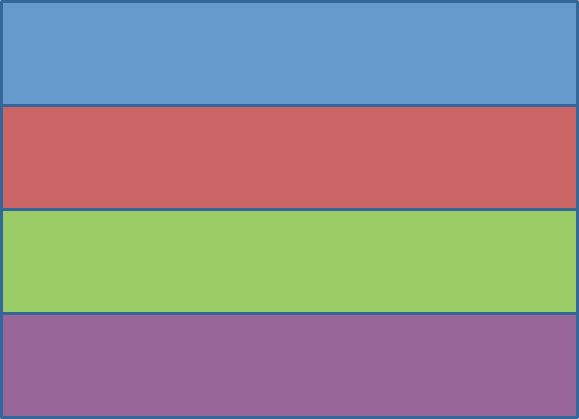
\includegraphics[height=5cm,width=\textwidth]{pics/dmat_block}
                \caption{Block}
        \end{subfigure}
        \hspace{.1cm}
        \begin{subfigure}[b]{0.3\textwidth}
                \centering
                
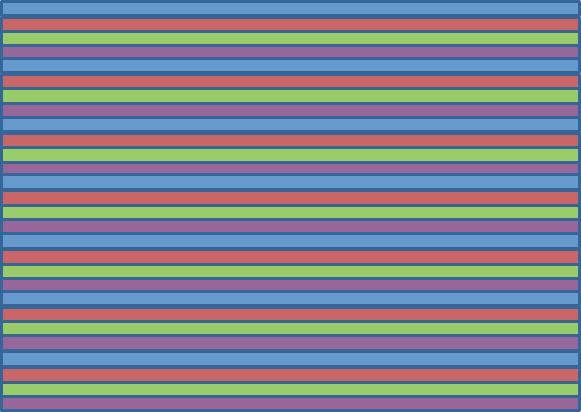
\includegraphics[height=5cm,width=\textwidth]{pics/dmat_cyclic}
                \caption{Cyclic}
        \end{subfigure}
        \hspace{.01cm}
        \begin{subfigure}[b]{0.3\textwidth}
                \centering
                
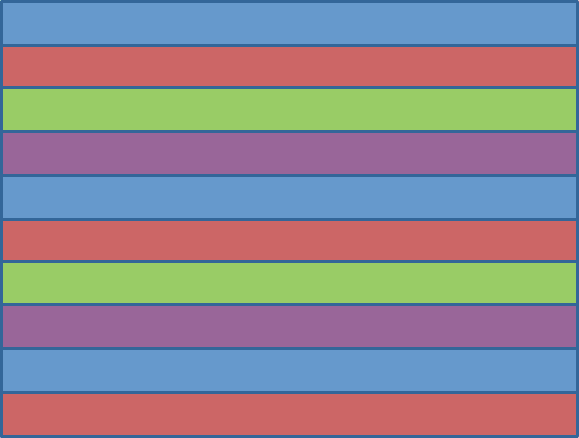
\includegraphics[height=5cm,width=\textwidth]{pics/dmat_blockcyclic}
                \caption{Block-Cyclic}
        \end{subfigure}
        \caption{Matrix Distribution Schemes}\label{fig:dmat1d}
\end{figure}
\end{block}
\end{frame}



\begin{frame}
\begin{block}{Distributed Matrices}
\begin{figure}[ht]
        \centering
        \begin{subfigure}[b]{0.3\textwidth}
                \centering
                
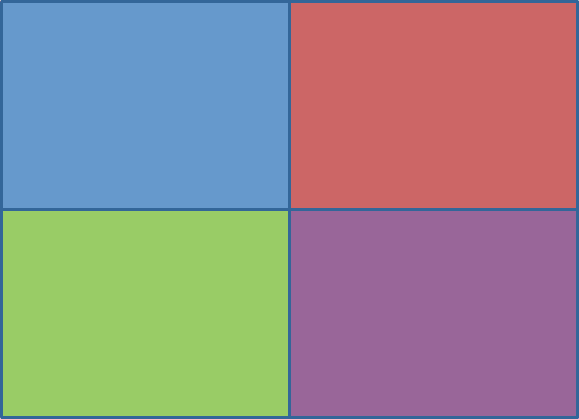
\includegraphics[height=5cm,width=\textwidth]{pics/dmat_block2d}
                \caption{2d Block}
        \end{subfigure}%
        \hspace{.1cm}
        \begin{subfigure}[b]{0.3\textwidth}
                \centering
                
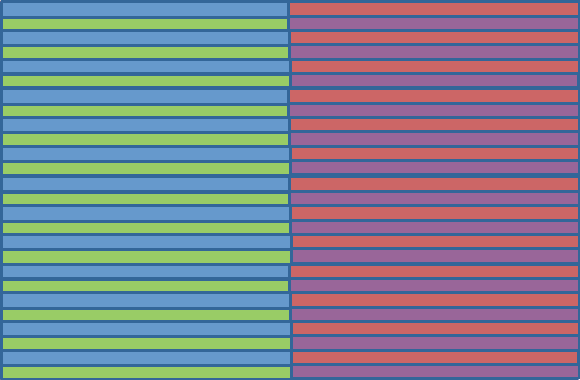
\includegraphics[height=5cm,width=\textwidth]{pics/dmat_cyclic2d}
                \caption{2d Cyclic}
        \end{subfigure}
        \hspace{.01cm}
        \begin{subfigure}[b]{0.3\textwidth}
                \centering
                
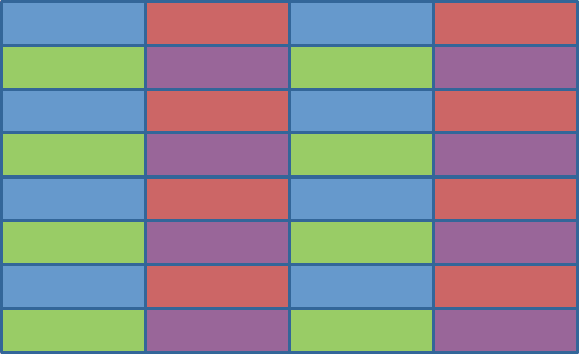
\includegraphics[height=5cm,width=\textwidth]{pics/dmat_blockcyclic2d}
                \caption{2d Block-Cyclic}
        \end{subfigure}
        \caption{Matrix Distribution Schemes Onto a 2-Dimensional 
Grid}\label{fig:dmat2d}
\end{figure}
\end{block}
\end{frame}



\begin{frame}
\begin{block}{Processor Grid Shapes}
\begin{table}[ht]
        \centering
        \begin{subfigure}[b]{0.23\textwidth}
                \centering
              $\left[\begin{tabular}{l}
                  0 \\ 1 \\ 2 \\ 3 \\ 4 \\ 5
                \end{tabular}\right]^T$
                \caption{$1\times 6$}
        \end{subfigure}
        \begin{subfigure}[b]{0.23\textwidth}
                \centering
                $\left[\begin{tabular}{lll}
                  0 & 1 & 2\\
                  3 & 4 & 5
                \end{tabular}\right]$
                \caption{$2\times 3$}
        \end{subfigure}%
        \begin{subfigure}[b]{0.23\textwidth}
                \centering
              $\left[\begin{tabular}{ll}
                  0 & 1 \\
                  2 & 3\\
                  4 & 5
                \end{tabular}\right]$
                \caption{$3\times 2$}
        \end{subfigure}
        \begin{subfigure}[b]{0.23\textwidth}
                \centering
              $\left[\begin{tabular}{l}
                  0 \\ 1 \\ 2 \\ 3 \\ 4 \\ 5
                \end{tabular}\right]$
                \caption{$6\times 1$}
        \end{subfigure}
        \caption{Processor Grid Shapes with 6 Processors}\label{fig:gridshapes}
\end{table}
\end{block}
\end{frame}





\begin{frame}
  \begin{block}{Distributed Matrices}\pause
  The data structure is a special R class (in the OOP sense) called 
\code{ddmatrix}.  It is the ``under the rug'' storage for a block-cyclic matrix 
distributed onto a 2-dimensional processor grid.\\[.4cm]
{\tiny
\begin{align*}
\hspace{.1cm}\text{\code{ddmatrix}}&=\begin{cases}
 $\textbf{Data}$ & $S4 local submatrix, an R matrix$\\
 $\textbf{dim}$ & $S4 dimension of the global matrix, a numeric pair$\\
 $\textbf{ldim}$ & $S4 dimension of the local submatrix, a numeric pair$\\
 $\textbf{bldim}$ & $S4 ScaLAPACK blocking factor, a numeric pair$\\
 $\textbf{CTXT}$ & $S4 BLACS context, an numeric singleton$
 \end{cases}
\end{align*}
}with prototype{\tiny
\begin{align*}
\hspace{-2.9cm}\text{\code{new("ddmatrix")}}&=\begin{cases}
 $\textbf{Data}$ & =\text{\code{matrix(0.0)}}\\
 $\textbf{dim}$ & =\text{\code{c(1,1)}}\\
 $\textbf{ldim}$ & =\text{\code{c(1,1)}}\\
 $\textbf{bldim}$ & =\text{\code{c(1,1)}}\\
 $\textbf{CTXT}$ & =\text{\code{0.0}}
 \end{cases}
\end{align*}
}
  \end{block}
\end{frame}


\begin{frame}
  \begin{block}{Distributed Matrices:  The Data Structure}\pause
      Example:  an $9\times 9$ matrix is distributed with a ``block-cycling'' 
factor of $2\times 2$ on a $2\times 2$ processor grid:
      \begin{center}
      \begin{minipage}{.45\textwidth}
      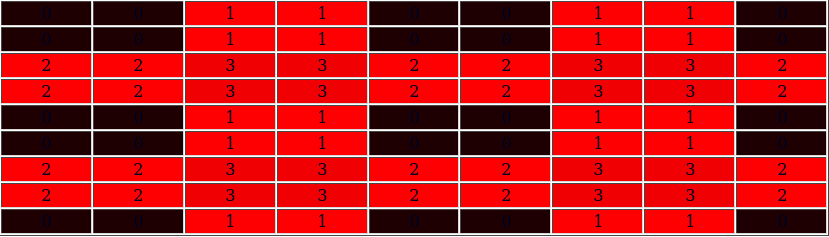
\includegraphics[width=5cm, height=4cm]{pics/dmat_dist}  
      \end{minipage}\hspace{.1cm}
      \begin{minipage}{.45\textwidth}
      \begin{center}
      \begin{align*}
        &=\begin{cases}
        $\textbf{Data}$ & =\text{\code{matrix(\dots)}}\\
        $\textbf{dim}$ & =\text{\code{c(9, 9)}}\\
        $\textbf{ldim}$ & =\text{\code{c(\dots)}}\\
        $\textbf{bldim}$ & =\text{\code{c(2, 2)}}\\
        $\textbf{CTXT}$ & =0
        \end{cases}
        \end{align*}
      \end{center}
      \end{minipage}
      \end{center}
    {\small See \url{http://acts.nersc.gov/scalapack/hands-on/datadist.html}}
  \end{block}



\subsection{DMAT Distributions}



\end{frame}

\begin{frame}
\begin{exampleblock}{Understanding Dmat: Global Matrix}
\begin{align*}
x &= \left[
      \begin{array}{lllllllll}
      x_{11} & x_{12} & x_{13} & x_{14} & x_{15} & x_{16} & x_{17} & x	_{18} & x_{19}\\
      x_{21} & x_{22} & x_{23} & x_{24} & x_{25} & x_{26} & x_{27} & x	_{28} & x_{29}\\
      x_{31} & x_{32} & x_{33} & x_{34} & x_{35} & x_{36} & x_{37} & x	_{38} & x_{39}\\
      x_{41} & x_{42} & x_{43} & x_{44} & x_{45} & x_{46} & x_{47} & x	_{48} & x_{49}\\
      x_{51} & x_{52} & x_{53} & x_{54} & x_{55} & x_{56} & x_{57} & x	_{58} & x_{59}\\
      x_{61} & x_{62} & x_{63} & x_{64} & x_{65} & x_{66} & x_{67} & x	_{68} & x_{69}\\
      x_{71} & x_{72} & x_{73} & x_{74} & x_{75} & x_{76} & x_{77} & x	_{78} & x_{79}\\
      x_{81} & x_{82} & x_{83} & x_{84} & x_{85} & x_{86} & x_{87} & x	_{88} & x_{89}\\
      x_{91} & x_{92} & x_{93} & x_{94} & x_{95} & x_{96} & x_{97} & x	_{98} & x_{99}
      \end{array}
\right]_{9\times 9}
\end{align*}
\end{exampleblock}
\end{frame}



\begin{frame}
\begin{exampleblock}{DMAT:  1-dimensional Row Block}
\begin{align*}
x &= \left[
      \begin{array}{lllllllll}
      \color{g11}x_{11} & \color{g11}x_{12} & \color{g11}x_{13} & 
\color{g11}x_{14} & \color{g11}x_{15} & \color{g11}x_{16} & \color{g11}x_{17} & 
\color{g11}x_{18} & \color{g11}x_{19}\\
      \color{g11}x_{21} & \color{g11}x_{22} & \color{g11}x_{23} & 
\color{g11}x_{24} & \color{g11}x_{25} & \color{g11}x_{26} & \color{g11}x_{27} & 
\color{g11}x_{28} & \color{g11}x_{29}\\
      \color{g11}x_{31} & \color{g11}x_{32} & \color{g11}x_{33} & 
\color{g11}x_{34} & \color{g11}x_{35} & \color{g11}x_{36} & \color{g11}x_{37} & 
\color{g11}x_{38} & \color{g11}x_{39}\\\hline
      \color{g12}x_{41} & \color{g12}x_{42} & \color{g12}x_{43} & 
\color{g12}x_{44} & \color{g12}x_{45} & \color{g12}x_{46} & \color{g12}x_{47} & 
\color{g12}x_{48} & \color{g12}x_{49}\\
      \color{g12}x_{51} & \color{g12}x_{52} & \color{g12}x_{53} & 
\color{g12}x_{54} & \color{g12}x_{55} & \color{g12}x_{56} & \color{g12}x_{57} & 
\color{g12}x_{58} & \color{g12}x_{59}\\
      \color{g12}x_{61} & \color{g12}x_{62} & \color{g12}x_{63} & 
\color{g12}x_{64} & \color{g12}x_{65} & \color{g12}x_{66} & \color{g12}x_{67} & 
\color{g12}x_{68} & \color{g12}x_{69}\\\hline
      \color{g13}x_{71} & \color{g13}x_{72} & \color{g13}x_{73} & 
\color{g13}x_{74} & \color{g13}x_{75} & \color{g13}x_{76} & \color{g13}x_{77} & 
\color{g13}x_{78} & \color{g13}x_{79}\\
      \color{g13}x_{81} & \color{g13}x_{82} & \color{g13}x_{83} & 
\color{g13}x_{84} & \color{g13}x_{85} & \color{g13}x_{86} & \color{g13}x_{87} & 
\color{g13}x_{88} & \color{g13}x_{89}\\
      \color{g13}x_{91} & \color{g13}x_{92} & \color{g13}x_{93} & 
\color{g13}x_{94} & \color{g13}x_{95} & \color{g13}x_{96} & \color{g13}x_{97} & 
\color{g13}x_{98} & \color{g13}x_{99}\\
      \end{array}
\right]_{9\times 9}
\end{align*}
\begin{align*}
\text{Processor grid = }\left|
      \begin{array}{ll}
      \color{g11}0 & \color{g12}1 \\
      \color{g13}2 & \color{g21}3
      \end{array}
\right| &= 
\left|
      \begin{tabular}{lll}
      \color{g11}(0,0) & \color{g12}(0,1) \\
      \color{g13}(1,0) & \color{g21}(1,1) 
      \end{tabular}
\right|
\end{align*}
\end{exampleblock}
\end{frame}





\begin{frame}
\begin{exampleblock}{DMAT: 2-dimensional Row Block}
\begin{align*}
x &= \left[
      \begin{array}{lllll|llll}
      \color{g11}x_{11} & \color{g11}x_{12} & \color{g11}x_{13} & 
\color{g11}x_{14} & \color{g11}x_{15} & \color{g12}x_{16} & \color{g12}x_{17} & 
\color{g12}x_{18} & \color{g12}x_{19}\\
      \color{g11}x_{21} & \color{g11}x_{22} & \color{g11}x_{23} & 
\color{g11}x_{24} & \color{g11}x_{25} & \color{g12}x_{26} & \color{g12}x_{27} & 
\color{g12}x_{28} & \color{g12}x_{29}\\
      \color{g11}x_{31} & \color{g11}x_{32} & \color{g11}x_{33} & 
\color{g11}x_{34} & \color{g11}x_{35} & \color{g12}x_{36} & \color{g12}x_{37} & 
\color{g12}x_{38} & \color{g12}x_{39}\\
      \color{g11}x_{41} & \color{g11}x_{42} & \color{g11}x_{43} & 
\color{g11}x_{44} & \color{g11}x_{45} & \color{g12}x_{46} & \color{g12}x_{47} & 
\color{g12}x_{48} & \color{g12}x_{49}\\
      \color{g11}x_{51} & \color{g11}x_{52} & \color{g11}x_{53} & 
\color{g11}x_{54} & \color{g11}x_{55} & \color{g12}x_{56} & \color{g12}x_{57} & 
\color{g12}x_{58} & \color{g12}x_{59}\\\hline
      \color{g13}x_{61} & \color{g13}x_{62} & \color{g13}x_{63} & 
\color{g13}x_{64} & \color{g13}x_{65} & \color{g21}x_{66} & \color{g21}x_{67} & 
\color{g21}x_{68} & \color{g21}x_{69}\\
      \color{g13}x_{71} & \color{g13}x_{72} & \color{g13}x_{73} & 
\color{g13}x_{74} & \color{g13}x_{75} & \color{g21}x_{76} & \color{g21}x_{77} & 
\color{g21}x_{78} & \color{g21}x_{79}\\
      \color{g13}x_{81} & \color{g13}x_{82} & \color{g13}x_{83} & 
\color{g13}x_{84} & \color{g13}x_{85} & \color{g21}x_{86} & \color{g21}x_{87} & 
\color{g21}x_{88} & \color{g21}x_{89}\\
      \color{g13}x_{91} & \color{g13}x_{92} & \color{g13}x_{93} & 
\color{g13}x_{94} & \color{g13}x_{95} & \color{g21}x_{96} & \color{g21}x_{97} & 
\color{g21}x_{98} & \color{g21}x_{99}\\
      \end{array}
\right]_{9\times 9}
\end{align*}
\begin{align*}
\text{Processor grid = }\left|
      \begin{array}{ll}
      \color{g11}0 & \color{g12}1 \\
      \color{g13}2 & \color{g21}3
      \end{array}
\right| &= 
\left|
      \begin{tabular}{lll}
      \color{g11}(0,0) & \color{g12}(0,1) \\
      \color{g13}(1,0) & \color{g21}(1,1) 
      \end{tabular}
\right|
\end{align*}
\end{exampleblock}
\end{frame}



\begin{frame}
\begin{exampleblock}{DMAT: 1-dimensional Row Cyclic}
\begin{align*}
x &= \left[
      \begin{array}{lllllllll}
      \color{g11}x_{11} & \color{g11}x_{12} & \color{g11}x_{13} & 
\color{g11}x_{14} & \color{g11}x_{15} & \color{g11}x_{16} & \color{g11}x_{17} & 
\color{g11}x_{18} & \color{g11}x_{19}\\\hline
      \color{g12}x_{21} & \color{g12}x_{22} & \color{g12}x_{23} & 
\color{g12}x_{24} & \color{g12}x_{25} & \color{g12}x_{26} & \color{g12}x_{27} & 
\color{g12}x_{28} & \color{g12}x_{29}\\\hline
      \color{g13}x_{31} & \color{g13}x_{32} & \color{g13}x_{33} & 
\color{g13}x_{34} & \color{g13}x_{35} & \color{g13}x_{36} & \color{g13}x_{37} & 
\color{g13}x_{38} & \color{g13}x_{39}\\\hline
      \color{g21}x_{41} & \color{g21}x_{42} & \color{g21}x_{43} & 
\color{g21}x_{44} & \color{g21}x_{45} & \color{g21}x_{46} & \color{g21}x_{47} & 
\color{g21}x_{48} & \color{g21}x_{49}\\\hline
      \color{g11}x_{51} & \color{g11}x_{52} & \color{g11}x_{53} & 
\color{g11}x_{54} & \color{g11}x_{55} & \color{g11}x_{56} & \color{g11}x_{57} & 
\color{g11}x_{58} & \color{g11}x_{59}\\\hline
      \color{g12}x_{61} & \color{g12}x_{62} & \color{g12}x_{63} & 
\color{g12}x_{64} & \color{g12}x_{65} & \color{g12}x_{66} & \color{g12}x_{67} & 
\color{g12}x_{68} & \color{g12}x_{69}\\\hline
      \color{g13}x_{71} & \color{g13}x_{72} & \color{g13}x_{73} & 
\color{g13}x_{74} & \color{g13}x_{75} & \color{g13}x_{76} & \color{g13}x_{77} & 
\color{g13}x_{78} & \color{g13}x_{79}\\\hline
      \color{g21}x_{81} & \color{g21}x_{82} & \color{g21}x_{83} & 
\color{g21}x_{84} & \color{g21}x_{85} & \color{g21}x_{86} & \color{g21}x_{87} & 
\color{g21}x_{88} & \color{g21}x_{89}\\\hline
      \color{g11}x_{91} & \color{g11}x_{92} & \color{g11}x_{93} & 
\color{g11}x_{94} & \color{g11}x_{95} & \color{g11}x_{96} & \color{g11}x_{97} & 
\color{g11}x_{98} & \color{g11}x_{99}\\
      \end{array}
\right]_{9\times 9}
\end{align*}
\begin{align*}
\text{Processor grid = }\left|
      \begin{array}{ll}
      \color{g11}0 & \color{g12}1 \\
      \color{g13}2 & \color{g21}3
      \end{array}
\right| &= 
\left|
      \begin{tabular}{lll}
      \color{g11}(0,0) & \color{g12}(0,1) \\
      \color{g13}(1,0) & \color{g21}(1,1) 
      \end{tabular}
\right|
\end{align*}
\end{exampleblock}
\end{frame}



\begin{frame}
\begin{exampleblock}{DMAT: 2-dimensional Row Cyclic}
\begin{align*}
x &= \left[
      \begin{array}{lllll|llll}
      \color{g11}x_{11} & \color{g11}x_{12} & \color{g11}x_{13} & 
\color{g11}x_{14} & \color{g11}x_{15} & \color{g12}x_{16} & \color{g12}x_{17} & 
\color{g12}x_{18} & \color{g12}x_{19}\\\hline
      \color{g13}x_{21} & \color{g13}x_{22} & \color{g13}x_{23} & 
\color{g13}x_{24} & \color{g13}x_{25} & \color{g21}x_{26} & \color{g21}x_{27} & 
\color{g21}x_{28} & \color{g21}x_{29}\\\hline
      \color{g11}x_{31} & \color{g11}x_{32} & \color{g11}x_{33} & 
\color{g11}x_{34} & \color{g11}x_{35} & \color{g12}x_{36} & \color{g12}x_{37} & 
\color{g12}x_{38} & \color{g12}x_{39}\\\hline
      \color{g13}x_{41} & \color{g13}x_{42} & \color{g13}x_{43} & 
\color{g13}x_{44} & \color{g13}x_{45} & \color{g21}x_{46} & \color{g21}x_{47} & 
\color{g21}x_{48} & \color{g21}x_{49}\\\hline
      \color{g11}x_{51} & \color{g11}x_{52} & \color{g11}x_{53} & 
\color{g11}x_{54} & \color{g11}x_{55} & \color{g12}x_{56} & \color{g12}x_{57} & 
\color{g12}x_{58} & \color{g12}x_{59}\\\hline
      \color{g13}x_{61} & \color{g13}x_{62} & \color{g13}x_{63} & 
\color{g13}x_{64} & \color{g13}x_{65} & \color{g21}x_{66} & \color{g21}x_{67} & 
\color{g21}x_{68} & \color{g21}x_{69}\\\hline
      \color{g11}x_{71} & \color{g11}x_{72} & \color{g11}x_{73} & 
\color{g11}x_{74} & \color{g11}x_{75} & \color{g12}x_{76} & \color{g12}x_{77} & 
\color{g12}x_{78} & \color{g12}x_{79}\\\hline
      \color{g13}x_{81} & \color{g13}x_{82} & \color{g13}x_{83} & 
\color{g13}x_{84} & \color{g13}x_{85} & \color{g21}x_{86} & \color{g21}x_{87} & 
\color{g21}x_{88} & \color{g21}x_{89}\\\hline
      \color{g11}x_{91} & \color{g11}x_{92} & \color{g11}x_{93} & 
\color{g11}x_{94} & \color{g11}x_{95} & \color{g12}x_{96} & \color{g12}x_{97} & 
\color{g12}x_{98} & \color{g12}x_{99}\\
      \end{array}
\right]_{9\times 9}
\end{align*}
\begin{align*}
\text{Processor grid = }\left|
      \begin{array}{ll}
      \color{g11}0 & \color{g12}1 \\
      \color{g13}2 & \color{g21}3
      \end{array}
\right| &= 
\left|
      \begin{tabular}{lll}
      \color{g11}(0,0) & \color{g12}(0,1) \\
      \color{g13}(1,0) & \color{g21}(1,1) 
      \end{tabular}
\right|
\end{align*}
\end{exampleblock}
\end{frame}




\begin{frame}[shrink]
\begin{exampleblock}{DMAT: 2-dimensional Block-Cyclic}
\begin{align*}
x &= \left[
      \begin{array}{ll|ll|ll|ll|l}
      \color{g11}x_{11} & \color{g11}x_{12} & \color{g12}x_{13} & \color{g12}x_{14} & \color{g11}x_{15} & \color{g11}x_{16} & \color{g12}x_{17} & \color{g12}x_{18} & \color{g11}x_{19}\\
      \color{g11}x_{21} & \color{g11}x_{22} & \color{g12}x_{23} & \color{g12}x_{24} & \color{g11}x_{25} & \color{g11}x_{26} & \color{g12}x_{27} & \color{g12}x_{28} & \color{g11}x_{29}\\\hline
      \color{g13}x_{31} & \color{g13}x_{32} & \color{g21}x_{33} & \color{g21}x_{34} & \color{g13}x_{35} & \color{g13}x_{36} & \color{g21}x_{37} & \color{g21}x_{38} & \color{g13}x_{39}\\
      \color{g13}x_{41} & \color{g13}x_{42} & \color{g21}x_{43} & \color{g21}x_{44} & \color{g13}x_{45} & \color{g13}x_{46} & \color{g21}x_{47} & \color{g21}x_{48} & \color{g13}x_{49}\\\hline
      \color{g11}x_{51} & \color{g11}x_{52} & \color{g12}x_{53} & \color{g12}x_{54} & \color{g11}x_{55} & \color{g11}x_{56} & \color{g12}x_{57} & \color{g12}x_{58} & \color{g11}x_{59}\\
      \color{g11}x_{61} & \color{g11}x_{62} & \color{g12}x_{63} & \color{g12}x_{64} & \color{g11}x_{65} & \color{g11}x_{66} & \color{g12}x_{67} & \color{g12}x_{68} & \color{g11}x_{69}\\\hline
      \color{g13}x_{71} & \color{g13}x_{72} & \color{g21}x_{73} & \color{g21}x_{74} & \color{g13}x_{75} & \color{g13}x_{76} & \color{g21}x_{77} & \color{g21}x_{78} & \color{g13}x_{79}\\
      \color{g13}x_{81} & \color{g13}x_{82} & \color{g21}x_{83} & \color{g21}x_{84} & \color{g13}x_{85} & \color{g13}x_{86} & \color{g21}x_{87} & \color{g21}x_{88} & \color{g13}x_{89}\\\hline
      \color{g11}x_{91} & \color{g11}x_{92} & \color{g12}x_{93} & \color{g12}x_{94} & \color{g11}x_{95} & \color{g11}x_{96} & \color{g12}x_{97} & \color{g12}x_{98} & \color{g11}x_{99}\\
      \end{array}
\right]_{9\times 9}
\end{align*}
\begin{align*}
\text{Processor grid = }\left|
      \begin{array}{ll}
      \color{g11}0 & \color{g12}1 \\
      \color{g13}2 & \color{g21}3
      \end{array}
\right| &= 
\left|
      \begin{tabular}{lll}
      \color{g11}(0,0) & \color{g12}(0,1) \\
      \color{g13}(1,0) & \color{g21}(1,1) 
      \end{tabular}
\right|
\end{align*}
\end{exampleblock}
\end{frame}



\begin{frame}[shrink]
\begin{exampleblock}{Understanding DMAT: Distributed with \text{\code{bldim} = (2,2)}}
\begin{align*}
x &= \left[
      \begin{array}{ll|ll|ll|ll|l}
      \color{g11}x_{11} & \color{g11}x_{12} & \color{g12}x_{13} & \color{g12}x_{14} & \color{g13}x_{15} & \color{g13}x_{16} & \color{g11}x_{17} & \color{g11}x_{18} & \color{g12}x_{19}\\
      \color{g11}x_{21} & \color{g11}x_{22} & \color{g12}x_{23} & \color{g12}x_{24} & \color{g13}x_{25} & \color{g13}x_{26} & \color{g11}x_{27} & \color{g11}x_{28} & \color{g12}x_{29}\\\hline
      \color{g21}x_{31} & \color{g21}x_{32} & \color{g22}x_{33} & \color{g22}x_{34} & \color{g23}x_{35} & \color{g23}x_{36} & \color{g21}x_{37} & \color{g21}x_{38} & \color{g22}x_{39}\\
      \color{g21}x_{41} & \color{g21}x_{42} & \color{g22}x_{43} & \color{g22}x_{44} & \color{g23}x_{45} & \color{g23}x_{46} & \color{g21}x_{47} & \color{g21}x_{48} & \color{g22}x_{49}\\\hline
      \color{g11}x_{51} & \color{g11}x_{52} & \color{g12}x_{53} & \color{g12}x_{54} & \color{g13}x_{55} & \color{g13}x_{56} & \color{g11}x_{57} & \color{g11}x_{58} & \color{g12}x_{59}\\
      \color{g11}x_{61} & \color{g11}x_{62} & \color{g12}x_{63} & \color{g12}x_{64} & \color{g13}x_{65} & \color{g13}x_{66} & \color{g11}x_{67} & \color{g11}x_{68} & \color{g12}x_{69}\\\hline
      \color{g21}x_{71} & \color{g21}x_{72} & \color{g22}x_{73} & \color{g22}x_{74} & \color{g23}x_{75} & \color{g23}x_{76} & \color{g21}x_{77} & \color{g21}x_{78} & \color{g22}x_{79}\\
      \color{g21}x_{81} & \color{g21}x_{82} & \color{g22}x_{83} & \color{g22}x_{84} & \color{g23}x_{85} & \color{g23}x_{86} & \color{g21}x_{87} & \color{g21}x_{88} & \color{g22}x_{89}\\\hline
      \color{g11}x_{91} & \color{g11}x_{92} & \color{g12}x_{93} & \color{g12}x_{94} & \color{g13}x_{95} & \color{g13}x_{96} & \color{g11}x_{97} & \color{g11}x_{98} & \color{g12}x_{99}\\
      \end{array}
\right]_{9\times 9}
\end{align*}
\begin{align*}
\text{Processor grid = }\left|
      \begin{array}{lll}
      \color{g11}0 & \color{g12}1 & \color{g13}2\\
      \color{g21}3 & \color{g22}4 & \color{g23}5
      \end{array}
\right| &= 
\left|
      \begin{tabular}{lll}
      \color{g11}(0,0) & \color{g12}(0,1) & \color{g13}(0,2)\\
      \color{g21}(1,0) & \color{g22}(1,1) & \color{g23}(1,2)
      \end{tabular}
\right|
\end{align*}
\end{exampleblock}
\end{frame}


\begin{frame}[shrink]
\begin{exampleblock}{Understanding DMAT: Local View}
\begin{align*}
\left[
      \begin{array}{ll|ll}
      \color{g11}x_{11} & \color{g11}x_{12} & \color{g11}x_{17} & \color{g11}x_{18}\\
      \color{g11}x_{21} & \color{g11}x_{22} & \color{g11}x_{27} & \color{g11}x_{28}\\\hline
      \color{g11}x_{51} & \color{g11}x_{52} & \color{g11}x_{57} & \color{g11}x_{58}\\
      \color{g11}x_{61} & \color{g11}x_{62} & \color{g11}x_{67} & \color{g11}x_{68}\\\hline
      \color{g11}x_{91} & \color{g11}x_{92} & \color{g11}x_{97} & \color{g11}x_{98}\\
      \end{array}
\right]_{5\times 4}
\left[
      \begin{array}{ll|l}
      \color{g12}x_{13} & \color{g12}x_{14} & \color{g12}x_{19}\\
      \color{g12}x_{23} & \color{g12}x_{24} & \color{g12}x_{29}\\\hline
      \color{g12}x_{53} & \color{g12}x_{54} & \color{g12}x_{59}\\
      \color{g12}x_{63} & \color{g12}x_{64} & \color{g12}x_{69}\\\hline
      \color{g12}x_{93} & \color{g12}x_{94} & \color{g12}x_{99}\\
      \end{array}
\right]_{5\times 3}
\left[
      \begin{array}{ll}
      \color{g13}x_{15} & \color{g13}x_{16}\\
      \color{g13}x_{25} & \color{g13}x_{26}\\\hline
      \color{g13}x_{55} & \color{g13}x_{56}\\
      \color{g13}x_{65} & \color{g13}x_{66}\\\hline
      \color{g13}x_{95} & \color{g13}x_{96}\\
      \end{array}
\right]_{5\times 2}
\\
\left[
      \begin{array}{ll|ll}
      \color{g21}x_{31} & \color{g21}x_{32} & \color{g21}x_{37} & \color{g21}x_{38}\\
      \color{g21}x_{41} & \color{g21}x_{42} & \color{g21}x_{47} & \color{g21}x_{48}\\\hline
      \color{g21}x_{71} & \color{g21}x_{72} & \color{g21}x_{77} & \color{g21}x_{78}\\
      \color{g21}x_{81} & \color{g21}x_{82} & \color{g21}x_{87} & \color{g21}x_{88}\\
      \end{array}
\right]_{4\times 4}
\left[
      \begin{array}{ll|l}
      \color{g22}x_{33} & \color{g22}x_{34} & \color{g22}x_{39}\\
      \color{g22}x_{43} & \color{g22}x_{44} & \color{g22}x_{49}\\\hline
      \color{g22}x_{73} & \color{g22}x_{74} & \color{g22}x_{79}\\
      \color{g22}x_{83} & \color{g22}x_{84} & \color{g22}x_{89}\\
      \end{array}
\right]_{4\times 3}
\left[
      \begin{array}{ll}
      \color{g23}x_{35} & \color{g23}x_{36} \\
      \color{g23}x_{45} & \color{g23}x_{46} \\\hline
      \color{g23}x_{75} & \color{g23}x_{76} \\
      \color{g23}x_{85} & \color{g23}x_{86} \\
      \end{array}
\right]_{4\times 2}
\end{align*}
\begin{align*}
\text{Processor grid = }\left|
      \begin{array}{lll}
      \color{g11}0 & \color{g12}1 & \color{g13}2\\
      \color{g21}3 & \color{g22}4 & \color{g23}5
      \end{array}
\right| &= 
\left|
      \begin{tabular}{lll}
      \color{g11}(0,0) & \color{g12}(0,1) & \color{g13}(0,2)\\
      \color{g21}(1,0) & \color{g22}(1,1) & \color{g23}(1,2)
      \end{tabular}
\right|
\end{align*}
\end{exampleblock}
\end{frame}

\begin{frame}[fragile]
  \begin{block}{The \code{DMAT} Data Structure}\pause
  \begin{enumerate}
    \item \code{DMAT} is \emph{distributed}.  No one processor owns all of the matrix.
%     \item \code{DMAT} makes no effort to load balance except for large objects.  Different processors can own different amounts of data.
    \item \code{DMAT} is \emph{non-overlapping}. Any piece owned by one processor is owned by no other processors.\\\hrule
    \item \code{DMAT} can be row-contiguous or not, depending on the blocking factor used.
    \item \code{DMAT} is locally column-major and globally, it depends\dots
    \item If \code{bldim[2] > ncol(X)} and \code{bldim[1] > nrow(X) / comm.size()} then \code{SPMD} is a generalization of \code{DMAT}.  Otherwise, no relation.
    \item \code{DMAT} is confusing, but very robust.
  \end{enumerate}
  \end{block}
\end{frame}


\begin{frame}
  \begin{block}{Pros and Cons of This Data Structure}\pause
  \begin{center}
    \begin{minipage}[t]{.45\textwidth}
      \begin{center}
      \begin{block}{Pros}
	\begin{itemize}
	\item Fast for distributed matrix computations
	\end{itemize}
      \end{block}
      \end{center}
    \end{minipage}\hspace{.5cm}
    \begin{minipage}[t]{.45\textwidth}
      \begin{center}
      \begin{block}{Cons}
	\begin{itemize}
	  \item Literally everything else
	\end{itemize}
      \end{block}
      \end{center}
    \end{minipage}
    \\[.6cm]
    \emph{This is why we hide most of the distributed details.}
    \\[.4cm]
    The details are there if you want them (you don't want them).
  \end{center}
  \end{block}
\end{frame}




\subsection{pbdDMAT}

\begin{frame}[fragile]
  \begin{block}{Distributed Matrix Methods}\pause
    \pkg{pbdDMAT} has over 100 methods with \emph{identical} syntax to R:
    \begin{itemize}
     \item \code{\`{}[\`{}}, \code{rbind()}, \code{cbind()}, \dots
     \item \code{lm.fit()}, \code{prcomp()}, \code{cov()}, \dots
     \item \code{\`{}\%*\%\`{}}, \code{solve()}, \code{svd()}, \code{norm()}, \dots
     \item \code{median()}, \code{mean()}, \code{rowSums()}, \dots
    \end{itemize}
\begin{lstlisting}[title=Serial Code]
cov(x)
\end{lstlisting}
  
\begin{lstlisting}[title=Parallel Code]
cov(x)
\end{lstlisting}
  \end{block}
\end{frame}

\begin{frame}[fragile]
  \begin{block}{Comparing pbdMPI and pbdDMAT}\pause
    \begin{itemize}
     \item \pkg{pbdMPI} is MPI $+$ some sugar.
     \item The \code{SPMD} data structure is not the only thing \pkg{pbdMPI} can handle (just a useful convention).
     \item \pkg{pbdDMAT} is more of a software package.
     \item The block-cyclic \code{DMAT} structure \emph{must} be used for \pkg{pbdDMAT}.
    \end{itemize}
  \end{block}
\end{frame}

\begin{frame}[fragile]
  \begin{block}{Quick Comments for Using pbdDMAT}\pause
    \begin{enumerate}
      \item Start by loading the package:
\vspace{-.4cm}
\begin{lstlisting}
library(pbdDMAT, quiet = TRUE)
\end{lstlisting}
      \item Always initialize before starting and finalize when finished:
\vspace{-.4cm}
\begin{lstlisting}
init.grid() # auto-calls pbdMPI's init()
# ...
finalize()
\end{lstlisting}
      \item Once you have your data in the right format, the code becomes identical to serial R code. The hard part is getting the data in the right format\dots
      \item   Distributed \code{DMAT} objects will be given the suffix \code{.dmat} to visually help distinguish them from global objects.  This suffix carries no semantic meaning.
    \end{enumerate}
  \end{block}
\end{frame}

















\section[pbdDMAT eg's]{Examples Using pbdDMAT}
\setcounter{excount}{0}



\subsection{pbdDMAT Example: Old Examples Revisited}

\begin{frame}[fragile]
  \begin{exampleblock}{Sample Covariance}\pause
\begin{lstlisting}[title=Serial Code]
Cov.X <- cov(X)
print(Cov.X)
\end{lstlisting}

\begin{lstlisting}[title=Parallel Code]
Cov.X <- cov(X)
print(Cov.X)
\end{lstlisting}
  \end{exampleblock}
\end{frame}

\begin{frame}[fragile,shrink]
  \begin{exampleblock}{Linear Regression Code}\pause
\begin{lstlisting}[title=Serial Code]
tX <- t(X)
A <- tX %*% X
B <- tX %*% y

ols <- solve(A) %*% B

# or
ols <- lm.fit(X, y)
\end{lstlisting}
  
\begin{lstlisting}[title=Parallel Code]
tX <- t(X)
A <- tX %*% X
B <- tX %*% y

ols <- solve(A) %*% B

# or
ols <- lm.fit(X, y)
\end{lstlisting}
  \end{exampleblock}
\end{frame}





\subsection{pbdDMAT Example: Generating Data}

\begin{frame}
  \begin{block}{Generating Random Data}\pause
    Using randomly generated matrices is the best way to ``get your feet wet'' with the pbd tools.  You can do this in 2 ways:
    \begin{enumerate}
     \item Generate a global matrix and distribute it.
     \item Generate locally only what is needed.
    \end{enumerate}
  \end{block}
\end{frame}

\begin{frame}[fragile,shrink]
  \begin{exampleblock}{Example \countex:  Random Distributed Matrix Generation}\pause
\begin{lstlisting}[title=Generate a global matrix and distribute it]
library(pbdDMAT, quiet=TRUE)
init.grid()

# Common global on all processors --> distributed
comm.set.seed(diff=FALSE)
x <- matrix(rnorm(100), nrow=10, ncol=10)
x.dmat <- as.ddmatrix(x)

# Global on processor 0 --> distributed
if (comm.rank()==0){
  x <- matrix(rnorm(100), nrow=10, ncol=10)
} else {
  x <- NULL
}
x.dmat <- as.ddmatrix(x)

finalize()
\end{lstlisting}
  \end{exampleblock}
\end{frame}

\begin{frame}[fragile]
  \begin{exampleblock}{Example \countex:  Random Distributed Matrix Generation}\pause
\begin{lstlisting}[title=Generate locally only what is needed]
library(pbdDMAT, quiet=TRUE)
init.grid()

comm.set.seed(diff = TRUE) # good seeds via rlecuyer
x.dmat <- ddmatrix("rnorm", nrow=10, ncol=10)

finalize()
\end{lstlisting}
  \end{exampleblock}
\end{frame}

\begin{frame}[fragile]
  \begin{exampleblock}{Example \countex:  Random Distributed Matrix Generation}\pause
\begin{lstlisting}[title=Generate locally only what is needed]
library(pbdDMAT, quiet=TRUE)
init.grid()

zero.dmat <- ddmatrix(0, nrow=100, ncol=100)
id.dmat <- diag(1, nrow=100, ncol=100)

finalize()
\end{lstlisting}
  \end{exampleblock}
\end{frame}




\subsection{pbdDMAT Example: Converting Between SPMD and DMAT}

\begin{frame}[fragile]
  \begin{exampleblock}{Example \countex:  Random Distributed Matrix Generation}\pause
\begin{lstlisting}[title=Convert between SPMD and DMAT]
library(pbdDEMO, quiet=TRUE)
init.grid()

comm.set.seed(diff = TRUE)

N.spmd <- 1 + comm.rank()
X.spmd <- matrix(rnorm(N.spmd * 3), ncol = 3)

# convert SPMD to DMAT
X.dmat <- spmd2dmat(X.spmd)

# convert DMAT to SPMD
new.X.spmd <- dmat2spmd(X.dmat)

# undistribute
X <- as.matrix(X.dmat)

finalize()
\end{lstlisting}
  \end{exampleblock}
\end{frame}



\begin{frame}
  \begin{block}{Distributed Matrices}\pause
  \begin{center}
    pbdDEMO contains many other examples of reading and managing SPMD and DMAT data
  \end{center}
  \end{block}
\end{frame}
% % % % \section[Iris]{In-Depth Example Examining the Iris Dataset with pbdR}
% % % % 
% % % % \hidenum
% % % % \begin{frame}[noframenumbering]
% % % % \frametitle{Contents}
% % % %  \tableofcontents[currentsection,hideothersubsections,sectionstyle=show/hide]
% % % % \end{frame}
% % % % \shownum
% % % % 
% % % % \subsection{Examining the Iris Dataset}
% % % % 
% % % % \begin{frame}[fragile]
% % % %   \begin{block}{The Iris Dataset}\pause
% % % % \begin{lstlisting}
% % % % rm(list = ls())                   # Clean environment
% % % % 
% % % % library(pbdMPI, quiet = TRUE)     # Load library
% % % % if(comm.size() != 4)
% % % %   comm.stop("4 processors are required.")
% % % % 
% % % % ### Load data
% % % % X <- as.matrix(iris[, -5])        # Dimension 150 by 4
% % % % X.cid <- as.numeric(iris[, 5])    # True id
% % % % 
% % % % ### Distribute data
% % % % jid <- get.jid(nrow(X))
% % % % X.spmd <- X[jid,]                 # SPMD row-major format
% % % % \end{lstlisting}
% % % % \end{block}
% % % % \end{frame}
% % % % 
% % % % 
% % % % \begin{frame}[fragile]
% % % %   \begin{block}{Standardizing}\pause
% % % % \begin{lstlisting}
% % % % ### Standardized
% % % % N <- allreduce(nrow(X.spmd))             # 150
% % % % p <- ncol(X.spmd)                        # 4
% % % % mu <- allreduce(colSums(X.spmd / N))
% % % % X.std <- sweep(X.spmd, 2, mu, FUN = "-") # Substract mean
% % % % std <- sqrt(allreduce(colSums(X.std^2 / (N - 1))))
% % % % X.std <- sweep(X.std, 2, std, FUN = "/") # Divide standard error
% % % % \end{lstlisting}
% % % % \end{block}
% % % % \end{frame}
% % % % 
% % % % \begin{frame}[fragile]
% % % %   \begin{block}{Projection Onto First 2 PC's}\pause
% % % % \begin{lstlisting}
% % % % ### SVD manually in serial
% % % % X.tmp <- crossprod(X.std)        # X'X (local)
% % % % X.tmp <- allreduce(X.tmp)
% % % % dim(X.tmp) <- c(p, p)
% % % % ret <- eigen(X.tmp)              # X'X = V D^2 V'
% % % % d <- sqrt(ret$values)
% % % % v <- ret$vectors
% % % % u <- X.std %*% v %*% diag(1/d)   # Why X V D^(-1)) = U?
% % % % \end{lstlisting}
% % % % \end{block}
% % % % \end{frame}
% % % % 
% % % % \subsection{Cluster}
% % % % 
% % % % \begin{frame}[fragile]
% % % %   \begin{block}{Clustering}\pause
% % % % \begin{lstlisting}
% % % % ### Clustering
% % % % set.seed(1234)                  # Set overall seed
% % % % X.kms <- kmeans(X.std, 3)       # K-means
% % % % X.kms
% % % % X.kms.cid <- X.kms$cluster      # Classification
% % % % 
% % % % library(EMCluster)              # Model-based clustering
% % % % X.mbc <- init.EM(X.std, 3)      # Initial by em-EM
% % % % X.mbc
% % % % X.mbc.cid <- X.mbc$class        # Classification
% % % % \end{lstlisting}
% % % % \end{block}
% % % % \end{frame}
% % % % 
% % % % \begin{frame}[fragile]
% % % %   \begin{block}{Cluster Validation}\pause
% % % % \begin{lstlisting}
% % % % ### Validation
% % % % X.kms.adjR <- RRand(X.cid, X.kms.cid)$adjRand       # Adjusted Rand index
% % % % X.mbc.adjR <- RRand(X.cid, X.mbc.cid)$adjRand
% % % % \end{lstlisting}
% % % % \end{block}
% % % % \end{frame}
% % % % 
% % % % \begin{frame}[fragile]
% % % %   \begin{block}{Cluster ID Variable}\pause
% % % % \begin{lstlisting}
% % % % ### Swap classification id
% % % % X.kms.cid[X.kms.cid == 2] <- 4
% % % % X.kms.cid[X.kms.cid == 3] <- 2
% % % % X.kms.cid[X.kms.cid == 4] <- 3
% % % % X.mbc.cid[X.mbc.cid == 2] <- 4
% % % % X.mbc.cid[X.mbc.cid == 3] <- 2
% % % % X.mbc.cid[X.mbc.cid == 4] <- 3
% % % % \end{lstlisting}
% % % % \end{block}
% % % % \end{frame}
% % % % 
% % % % \subsection{Plot}
% % % % 
% % % % \begin{frame}[fragile]
% % % %   \begin{block}{Plot}\pause
% % % % \begin{lstlisting}
% % % % ### Display on first 2 components
% % % % pdf("serial_plot.pdf")
% % % % 
% % % % par(mfrow = c(2, 2))
% % % % plot(X.prj, col = X.cid + 1, pch = X.cid,
% % % %      main = "iris (true)", xlab = "PC1", ylab = "PC2")
% % % % plot(X.prj, col = X.kms.cid + 1, pch = X.kms.cid,
% % % %      main = paste("iris (k-Means)", sprintf("%.4f", X.kms.adjR)),
% % % %      xlab = "PC1", ylab = "PC2")
% % % % plot(X.prj, col = X.mbc.cid + 1, pch = X.mbc.cid,
% % % %      main = paste("iris (Model-based)", sprintf("%.4f", X.mbc.adjR)),
% % % %      xlab = "PC1", ylab = "PC2")
% % % % accuracy <- c(X.kms.adjR, X.mbc.adjR)
% % % % names(accuracy) <- c("k-Means", "Model-based")
% % % % barplot(accuracy, main = "Clustering Accuracy")
% % % % 
% % % % dev.off()
% % % % \end{lstlisting}
% % % % \end{block}
% % % % \end{frame}
% % % % 
% % % % 
% % % % \begin{frame}
% % % %   \begin{block}{Plot}\pause
% % % % \begin{center}
% % % %   \includegraphics[scale=.37]{other/serial_plot.pdf}
% % % % \end{center}
% % % % \end{block}
% % % % \end{frame}


\section[Iris]{In-Depth Example Examining the Iris Dataset with pbdR}

\hidenum
\begin{frame}[noframenumbering]
\frametitle{Contents}
 \tableofcontents[currentsection,hideothersubsections,sectionstyle=show/hide]
\end{frame}
\shownum

\subsection{Examining the Iris Dataset}

\begin{frame}[fragile]
  \begin{block}{The Iris Dataset}\pause
\begin{lstlisting}
rm(list = ls())                    # Clean environment

library(pbdDMAT, quiet = TRUE)     # Load library
init.grid()
if(comm.size() != 4)
  comm.stop("4 processors are required.")

### Load data
X <- as.matrix(iris[, -5])         # Dimension 150 by 4
X.cid <- as.numeric(iris[, 5])     # True id

### Convert to ddmatrix
X.dmat <- as.ddmatrix(X)
\end{lstlisting}
\end{block}
\end{frame}


\begin{frame}[fragile]
  \begin{block}{Standardizing}\pause
\begin{lstlisting}
### Standardized
X.std <- scale(X.dmat)
mu <- as.matrix(colMeans(X.std))
cov <- as.matrix(cov(X.std))
comm.print(mu)
comm.print(cov)
\end{lstlisting}
\end{block}
\end{frame}

\begin{frame}[fragile]
  \begin{block}{Projection Onto First 2 PC's}\pause
\begin{lstlisting}
### SVD
X.svd <- svd(X.std)

### Project on column space of singular vectors
A <- X.svd$u %*% diag(X.svd$d, type="ddmatrix")
B <- X.std %*% X.svd$v            # A ~ B
X.prj <- as.matrix(A[, 1:2])      # Only useful for plot
\end{lstlisting}
\end{block}
\end{frame}

\subsection{Cluster}

\begin{frame}[fragile]
  \begin{block}{Clustering}\pause
\begin{lstlisting}
### Clustering
library(pmclust, quiet = TRUE)
comm.set.seed(123, diff = TRUE)

X.dmat <- X.std
PARAM.org <- set.global.dmat(K = 3)      # Preset storage
.pmclustEnv$CONTROL$debug <- 0           # Disable debug messages
PARAM.org <- initial.center.dmat(PARAM.org)
PARAM.kms <- kmeans.step.dmat(PARAM.org) # K-means
X.kms.cid <- as.vector(.pmclustEnv$CLASS.dmat)
\end{lstlisting}
\end{block}
\end{frame}

\begin{frame}[fragile]
  \begin{block}{Cluster Validation}\pause
\begin{lstlisting}
### Validation
X.kms.adjR <- EMCluster::RRand(X.cid, X.kms.cid)$adjRand
comm.print(X.kms.adjR)
\end{lstlisting}
\end{block}
\end{frame}

\begin{frame}[fragile]
  \begin{block}{Cluster ID Variable}\pause
\begin{lstlisting}
### Swap classification id
tmp <- X.kms.cid
X.kms.cid[tmp == 1] <- 3
X.kms.cid[tmp == 2] <- 1
X.kms.cid[tmp == 3] <- 2
\end{lstlisting}
\end{block}
\end{frame}

\subsection{Plot}

\begin{frame}[fragile]
  \begin{block}{Plot}\pause
\begin{lstlisting}
### Display on first 2 components
if(comm.rank() == 0){
  pdf("dmat_plot.pdf")
  
  par(mfrow = c(2, 2))
  plot(X.prj, col = X.cid + 1, pch = X.cid,
       main = "iris (true)", xlab = "PC1", ylab = "PC2")
  plot(X.prj, col = X.kms.cid + 1, pch = X.kms.cid,
       main = paste("iris (kmeans)", sprintf("%.4f", X.kms.adjR)),
       xlab = "PC1", ylab = "PC2")
  
  dev.off()
}
\end{lstlisting}
\end{block}
\end{frame}


\begin{frame}
  \begin{block}{Plot}\pause
\begin{center}
  \includegraphics[scale=.37]{other/dmat_plot.pdf}\\
 \vspace{-1cm}\url{http://www.nics.tennessee.edu/getting-an-allocation} 
\end{center}
\end{block}
\end{frame}
%%%%%%%%%%%%%%%%%%%%%%%%%%%%%%%%%%%%%%%%
%%     Last few slides
%%%%%%%%%%%%%%%%%%%%%%%%%%%%%%%%%%%%%%%%
\section{Wrapup}

\hidenum
\begin{frame}[noframenumbering]
\frametitle{Contents}
 \tableofcontents[currentsection,hideothersubsections,sectionstyle=show/hide]
\end{frame}
\shownum

\begin{frame}
  \begin{block}{Where to Learn More}
    \begin{enumerate}
      \item The \pkg{pbdDEMO} package\\
      \url{http://cran.r-project.org/web/packages/pbdDEMO/}\\
      Vignette: \url{http://goo.gl/eBsIh}
      \item Our Google Group:\\
        \url{http://group.r-pbd.org}
      \item Get an allocation with us!\\
        {\small \url{http://www.nics.tennessee.edu/getting-an-allocation}\\ }
    \end{enumerate}
\end{block}
\end{frame}


\section*{}


% \begin{frame}[fragile,allowframebreaks]
%   \tiny
%   \bibliographystyle{plainnat}
%   \bibliography{pbdbib}
% \end{frame}


\hidenum
\begin{frame}[noframenumbering]
 \begin{block}{Thanks for coming!}
 \begin{center}
     {\Large Questions?  Comments?}\\[.4cm]
     Please help us improve this tutorial by completing a short survey:\\
     \url{http://www.surveymonkey.com/s/W8VLJSP}
  \end{center}
 \end{block}
\end{frame}


\end{document}
%%%%%%%%%%%%%%%%%%%%%%%%%%%%%%%%